\cleardoublepage
\section{Event selection}
\label{sec:cr}


The preselection common to all regions (signal and control regions) is:

\begin{itemize}
\item exactly one CA15 fat jet with $\textit{p}_\text{T}>\text{200}$\,GeV and $|\eta|<\text{2.4}$ 
\item fat jet soft drop mass between 100 and 150\GeV
\item PF $\text{MET}>\text{250}$\,GeV (SR) or PF recoil $>\text{250}$\,GeV (CR) 
\item $\Delta \phi(\text{AK4~jets,MET/Recoil})>\text{0.4}$
\item $\tau$ and photon veto
\item not more than one additional AK4 jet
\item $N_2^\text{DDT}<0$
\end{itemize}

This already ensures a topology very close to the one expected by the monoH signal. Then lepton multiplicities and the number of b tagged AK4 jets which are not overlapping with the fat jet are used to distinguish between the signal and control regions in order to keep the extrapolation uncertainties at a minimum.

\begin{table}
  \begin{center}
  \caption{Event selection table. Common to all regions is a preselection} \label{tab:event_selection}
    \begin{tabular}{  l | c | c | c  }
      \hline \hline
        region   & iso AK4 b tags   & leptons & double-b  \\ \hline
        signal   & 0                & 0       & pass \\ \hline
        \ttbar   & 1                & 1       & pass/fail\\ \hline
        W        & 0                & 1       & pass/fail\\ \hline
        Dilepton & 0                & 2       & pass/fail\\
      \hline \hline
    \end{tabular}
  \end{center}
\end{table}


Finally, the control regions are split up into pass/fail regions depending on whether or not they pass the cut on the double-b tagger of $>0.75$ so that in total, we end up with 12 control regions ($[\text{t}\bar{\text{t}},\text{W},\text{Dilepton}]\times[e,\mu]\times[\text{pass,fail}]$). With respect to the other mono-X analyses, this analysis is not making use of a photon control region. The impact of having or removing such control region has been estimated to be of the order of a few \% on the overall mono-Higgs sensitivity. This is mainly due to the fact that the higher contribution of $t\bar{t}$ production to the overall background makes the impact of a tighter constrain on the $Z$+jets background, like the one given by the events with photons, less important for this search. Furthermore the simultaneous use of dilepton pass and fail control region enhances the statistical power, limiting the necessity of adding a high statistics control sample like the one composed by events with photons. Table~\ref{tab:event_selection} summarizes the selection. Key distributions for all the control regions are presented in Fig.~\ref{Fig_cr_ttbar_mu_1}-\ref{Fig_cr_dielectron_1}. In all distributions, MC is normalized to prediction. Recoil distributions are shown in Fig.~\ref{Fig_cr_Recoil}-\ref{Fig_cr_Recoil_fail}. In general, a very good shape agreement is observed. In the final fit, a scale factor is allowed to float that adjusts the relative normalization of the dominating backgrounds in the pass/fail categories. More details are given in Section~\ref{sec:results}. Finer binned versions of the recoil variables are presented in Fig.~\ref{Fig_cr_Recoil_fine}-\ref{Fig_cr_Recoil_fail_fine}.

Finally, the unblinded \ptmiss~distribution in the signal region is shown in Fig.~\ref{Fig_sr}. Fig.\ref{Fig_sr_content} in the Appendix gives more details as far as the quark content inside the fat jet for the main backgrounds is concerned. A slight excess is observed in events with higher \ptmiss. As the limits will show, this is compatible with SM background predictions within the 1$\sigma$ level once including all systematic uncertainties.

\clearpage

\begin{table}\footnotesize
\begin{center}
  \caption{Prefit event yield expectations for the \ttbar control regions. Uncertainties are statistical only.} \label{tab:yield_ttbar}
\begin{tabular}{l r  r r r}
  \hline\hline
Process       & \ttbar $\mu$   & \ttbar e     & \ttbar fail $\mu$  & \ttbar fail e\\ 
\hline
QCD           &$ 0.6 \pm 0.6  $&$ 0\pm0$      & $ 27.8 \pm 20.9  $ &$ 34.3\pm20.6$\\
DY            &$ 0.8 \pm 0.3 $ &$ 0.4\pm0.2$  & $ 20.4 \pm 1.9 $   &$ 6.5\pm1.0$\\
Diboson       &$ 1.1\pm0.8 $   &$ 0.4\pm0.4$  & $ 20.2\pm3.3 $     &$ 9.7\pm2.1$\\ 
SingleTop     &$ 26.3\pm2.1 $  &$ 16.1\pm1.6$ & $ 150.6\pm5.0 $    &$ 86.9\pm3.7$\\
W+jets        &$ 18.5\pm2.6 $  &$ 6.5\pm1.3$  & $ 471.4\pm13.4 $   &$ 274.3\pm9.9$\\
\ttbar        &$ 399.7\pm8.3 $ &$ 226.1\pm6.1$& $ 1984\pm19 $      &$ 1206\pm14$\\
SM H          &$ 1.2\pm 0.1  $ &$ 0.7\pm 0.1$ & $ 1.0 \pm 0.1$     &$ 0.7\pm 0.1$\\
\hline
Integral      &$ 447.7\pm9.0 $ &$ 249.8\pm6.5$& $ 2674\pm32 $      &$ 1618\pm27$\\
Data          &$ 425\pm20.6 $  &$ 246\pm15.7$ & $ 2626\pm51 $      &$ 1590\pm40$\\
\hline\hline
  \end{tabular}
\end{center}
\end{table}

\begin{table}\footnotesize
\begin{center}
  \caption{Prefit event yield expectations for the W control regions. Uncertainties are statistical only.} \label{tab:yield_w}
\begin{tabular}{l r  r r r}
  \hline\hline
Process         & W $\mu$               & W e                   &   W fail $\mu$  & W fail e                \\ 
\hline
QCD             &$ 8.8\pm6.3 $          &$ 0.9\pm0.7$           & $ 292.3\pm61.6 $&$ 141.7\pm37.7$\\
DY              &$ 12.1\pm1.6 $         &$ 3.7\pm0.8$           & $ 363.0\pm8.7 $&$ 97.3\pm4.5$\\
Diboson         &$ 11.4\pm2.3 $         &$ 7.1\pm1.8$           & $ 282.4\pm11.8 $&$ 154.8\pm8.6$\\ 
SingleTop       &$ 156.4\pm5.3 $        &$ 89.1\pm4.0$          & $ 664.4\pm11.0 $&$ 375.8\pm8.1$\\
W+jets          &$ 278.3\pm10.5 $       &$ 138.3\pm7.2$         & $ 10839\pm68 $&$ 5728\pm48$\\
\ttbar          &$ 672.8\pm11.1 $       &$ 405.6\pm8.4$         & $ 3202\pm24 $&$ 1990\pm19$\\
 SM H             &$ 19.0\pm0.2 $         & $ 12.2\pm0.2$         & $ 7.2\pm0.1 $& $ 4.3\pm0.1$\\ 
\hline
Integral        &$ 1159\pm18 $          &$ 656.8\pm12.0$        & $ 15650\pm96 $&$ 8492\pm65$\\
Data            &$ 1217\pm35 $          &$ 714\pm27$            & $ 17149\pm131 $&$ 9444\pm97$\\
\hline\hline
  \end{tabular}
\end{center}
\end{table}

\begin{table}\footnotesize
\begin{center}
  \caption{Prefit event yield expectations for the dilepton control region. Uncertainties are statistical only.} \label{tab:yield_dilepton}
\begin{tabular}{l r  r r r}
  \hline\hline
Process         & $\mu\mu$              & ee            & $\mu\mu$ fail & ee fail\\
\hline
Diboson         &$ 0.6\pm0.4  $         &$ 1.4\pm0.6$   & $ 28.0\pm3.2  $&$ 19.8\pm2.6$\\ 
SingleTop       &$1.8\pm0.6 $           &$ 1.2\pm0.4$   & $ 3.6\pm0.7 $&$ 2.5\pm0.6$\\
W+jets          &$ 0\pm0 $              &$ 0.4\pm0.4$   & $ 0.7\pm0.5 $&$ 1.5\pm0.7$\\
\ttbar          &$ 4.0\pm0.8 $          &$ 2.5\pm0.7$   & $ 21.1\pm2.0 $&$ 15.8\pm1.7$\\
DY              &$ 40.2\pm3.0 $         &$ 24.2\pm2.0$  & $ 1143\pm15 $&$ 756.0\pm12.2$\\
 SM H             &$ 3.3\pm0.1 $          &$ 2.3\pm0.1$   & $ 1.2\pm0.1 $&$ 0.8\pm0.1$\\ 
\hline
Integral        &$ 50.0\pm3.1 $         &$ 32.1\pm2.3$  & $ 1197\pm16 $&$ 796.4\pm12.6$\\
Data            &$ 54\pm7.3 $           &$ 42\pm6.5$    & $ 1373\pm37 $&$ 888\pm29.8$\\
\hline\hline
  \end{tabular}
\end{center}
\end{table}

\begin{table}\footnotesize
\begin{center}
  \caption{Prefit event yield expectations for the signal region. Uncertainties are statistical only.} \label{tab:yield_dilepton}
\begin{tabular}{l r}
  \hline\hline
Process         & Yields          \\
\hline
Diboson         &$ 27.0\pm3.1  $       \\
SingleTop       &$29.2\pm2.2 $         \\
W+jets          &$ 126.1\pm7.2 $            \\
\ttbar          &$ 271.7\pm7.1 $        \\
DY              &$ 303.9\pm6.8 $       \\
 SM H             &$ 29.0\pm0.2 $        \\
\hline
Integral        &$ 786.7\pm12.8 $       \\
Z'-2HDM 1.7\TeV ($m_{A^0}=300\GeV$)        &$ 69.8\pm0.6 $       \\
Data            & $ 913 \pm 30.2$         \\
\hline\hline
  \end{tabular}
\end{center}
\end{table}


\clearpage

\begin{figure}
\centering
 \subfloat{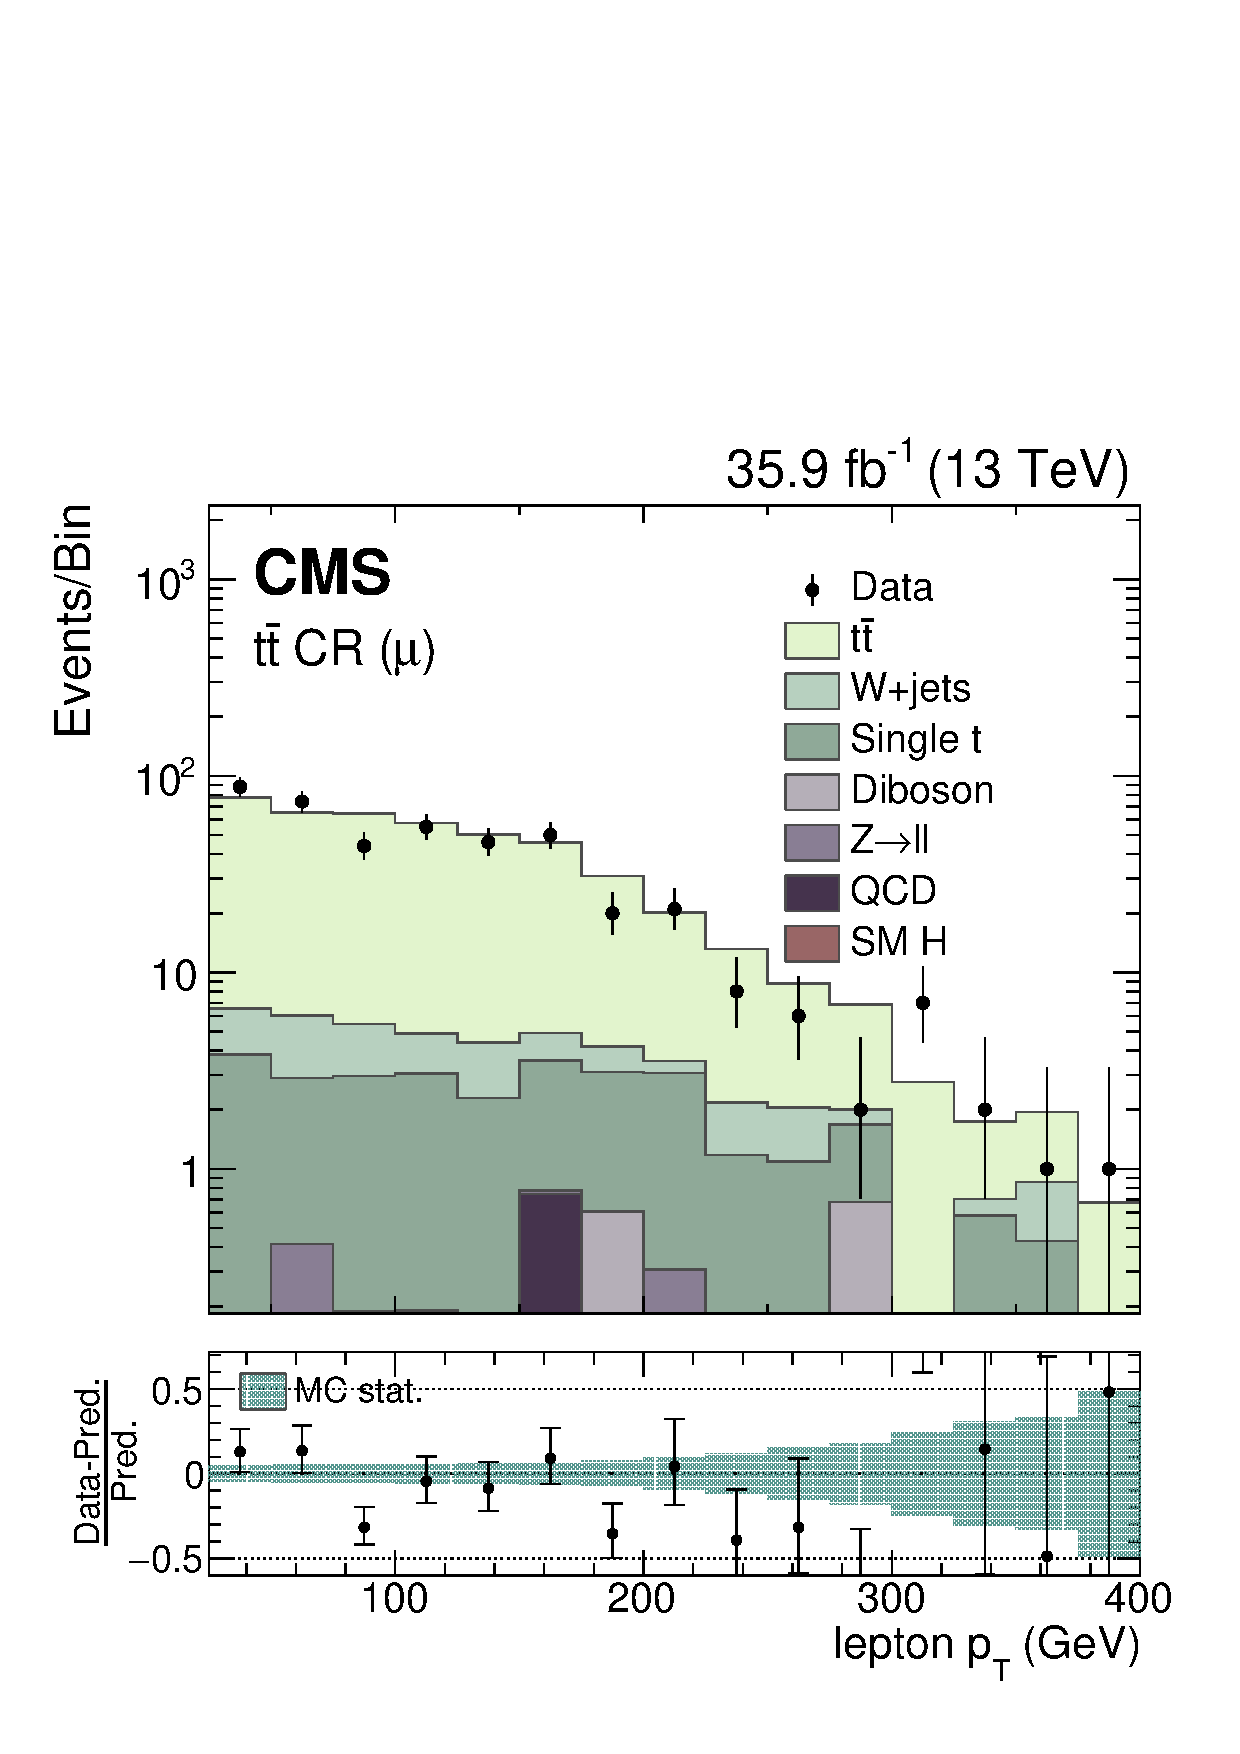
\includegraphics[width=0.4\textwidth]{figures/dataMC/cr_ttbar_mu_lep1Pt.pdf}}
 \subfloat{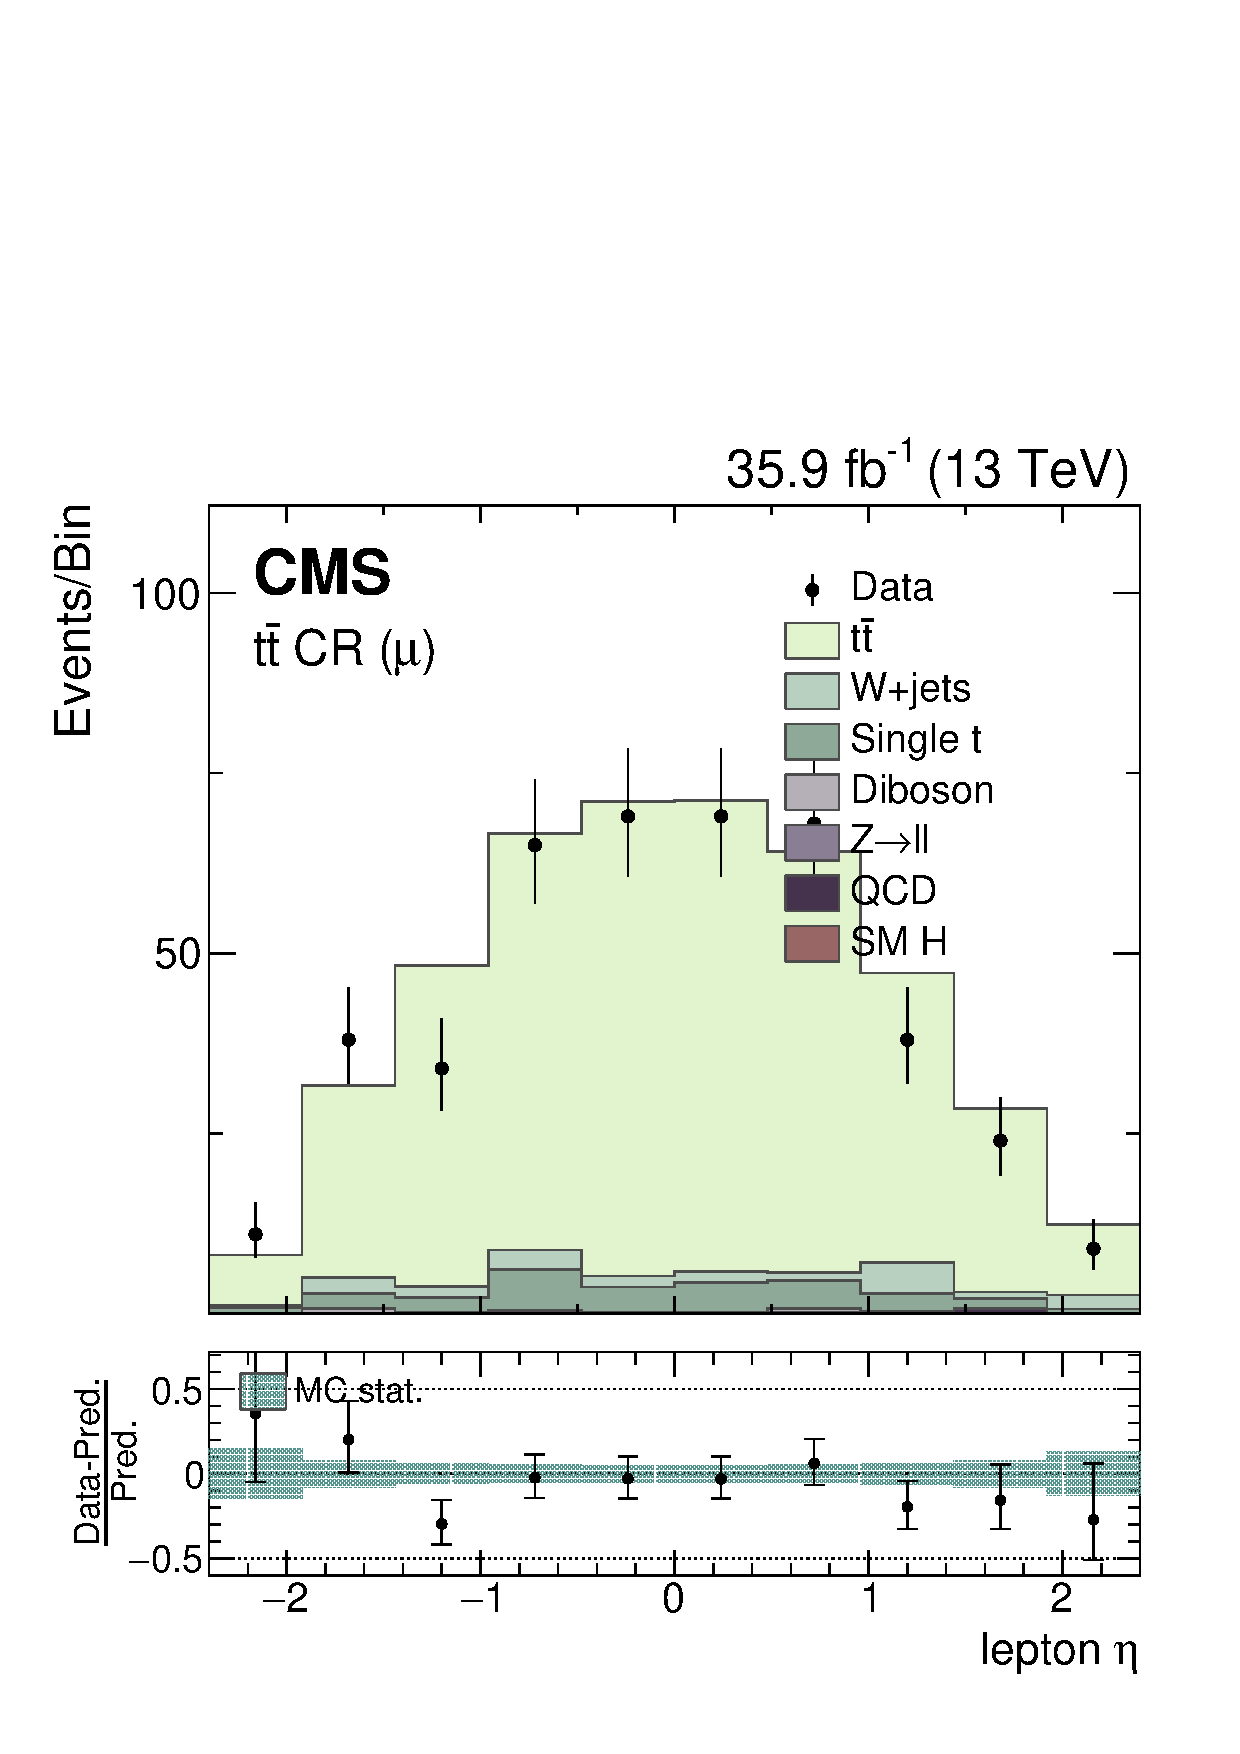
\includegraphics[width=0.4\textwidth]{figures/dataMC/cr_ttbar_mu_lep1Eta.pdf}} \\
 \subfloat{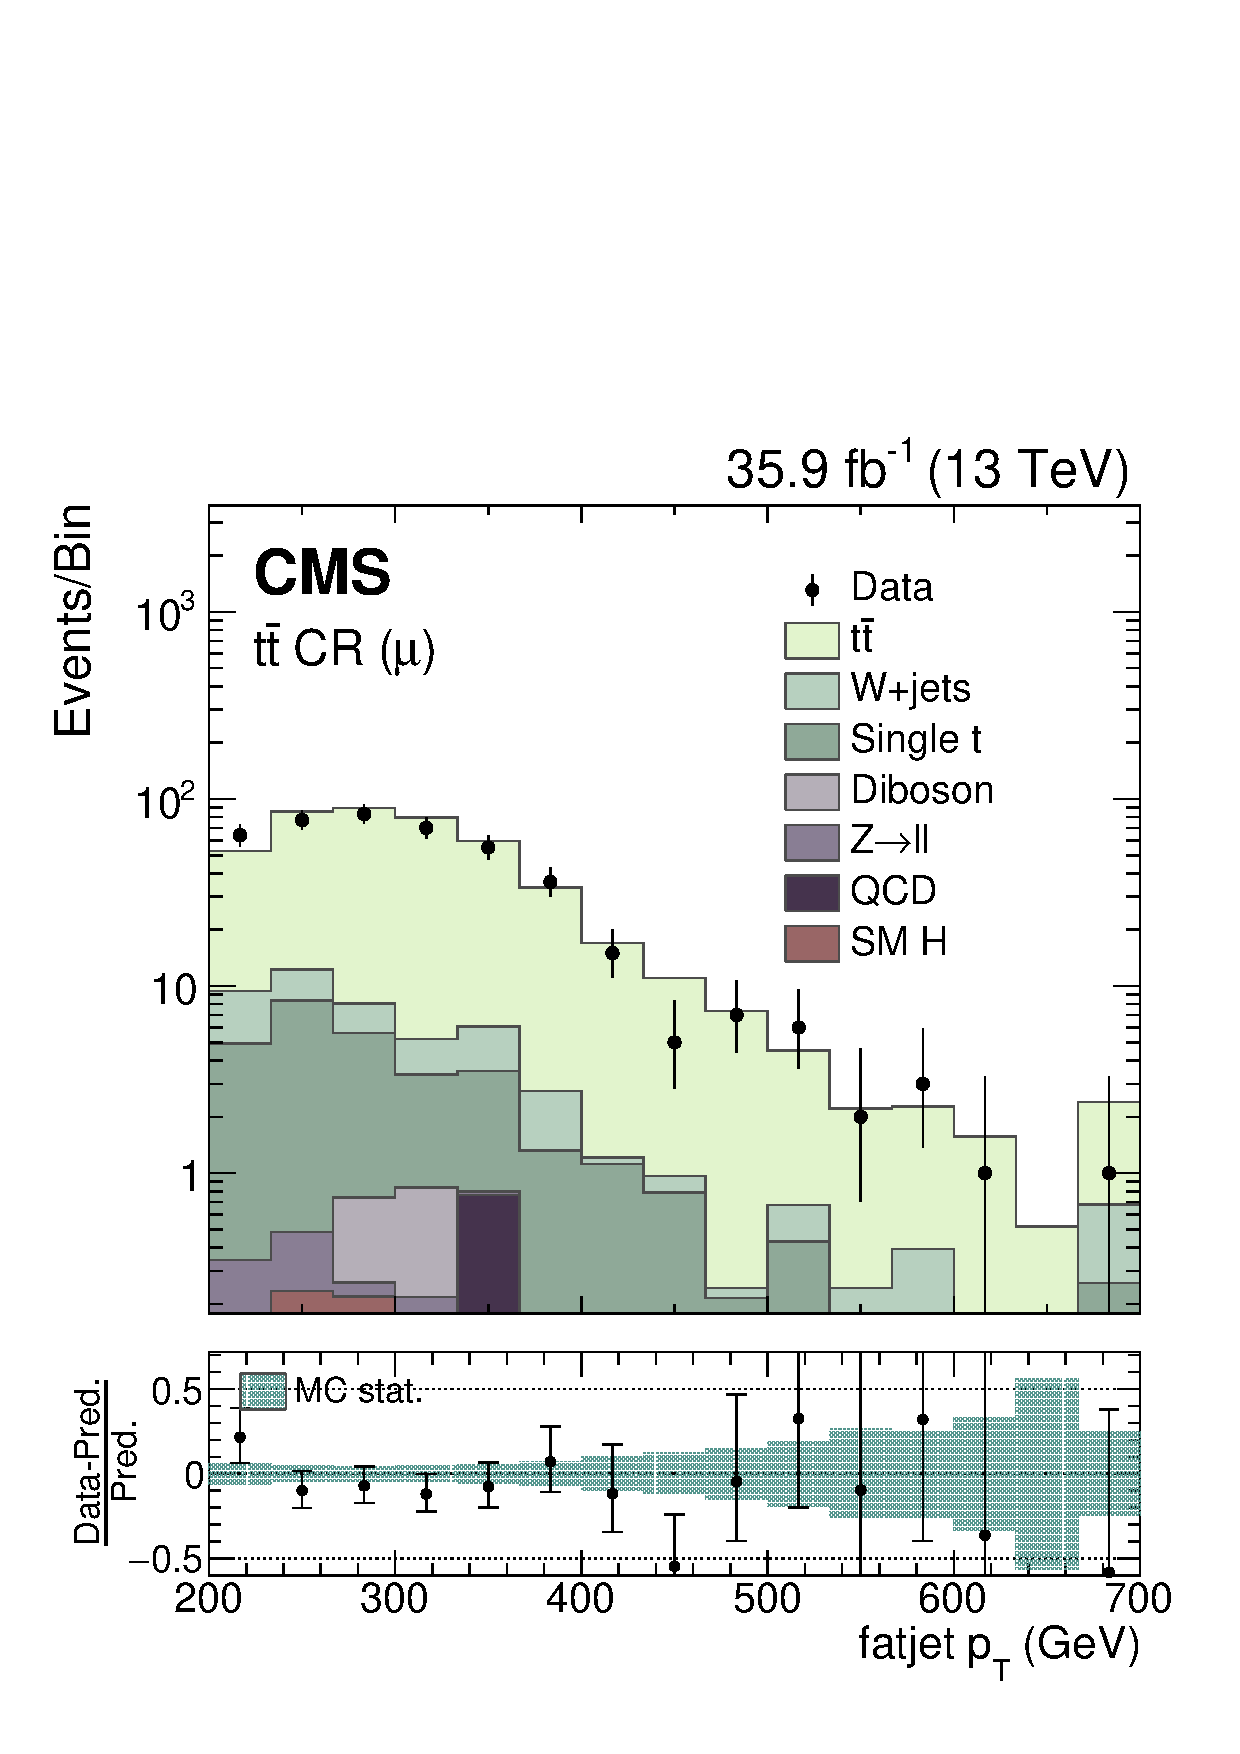
\includegraphics[width=0.4\textwidth]{figures/dataMC/cr_ttbar_mu_fj1Pt.pdf}}
 \subfloat{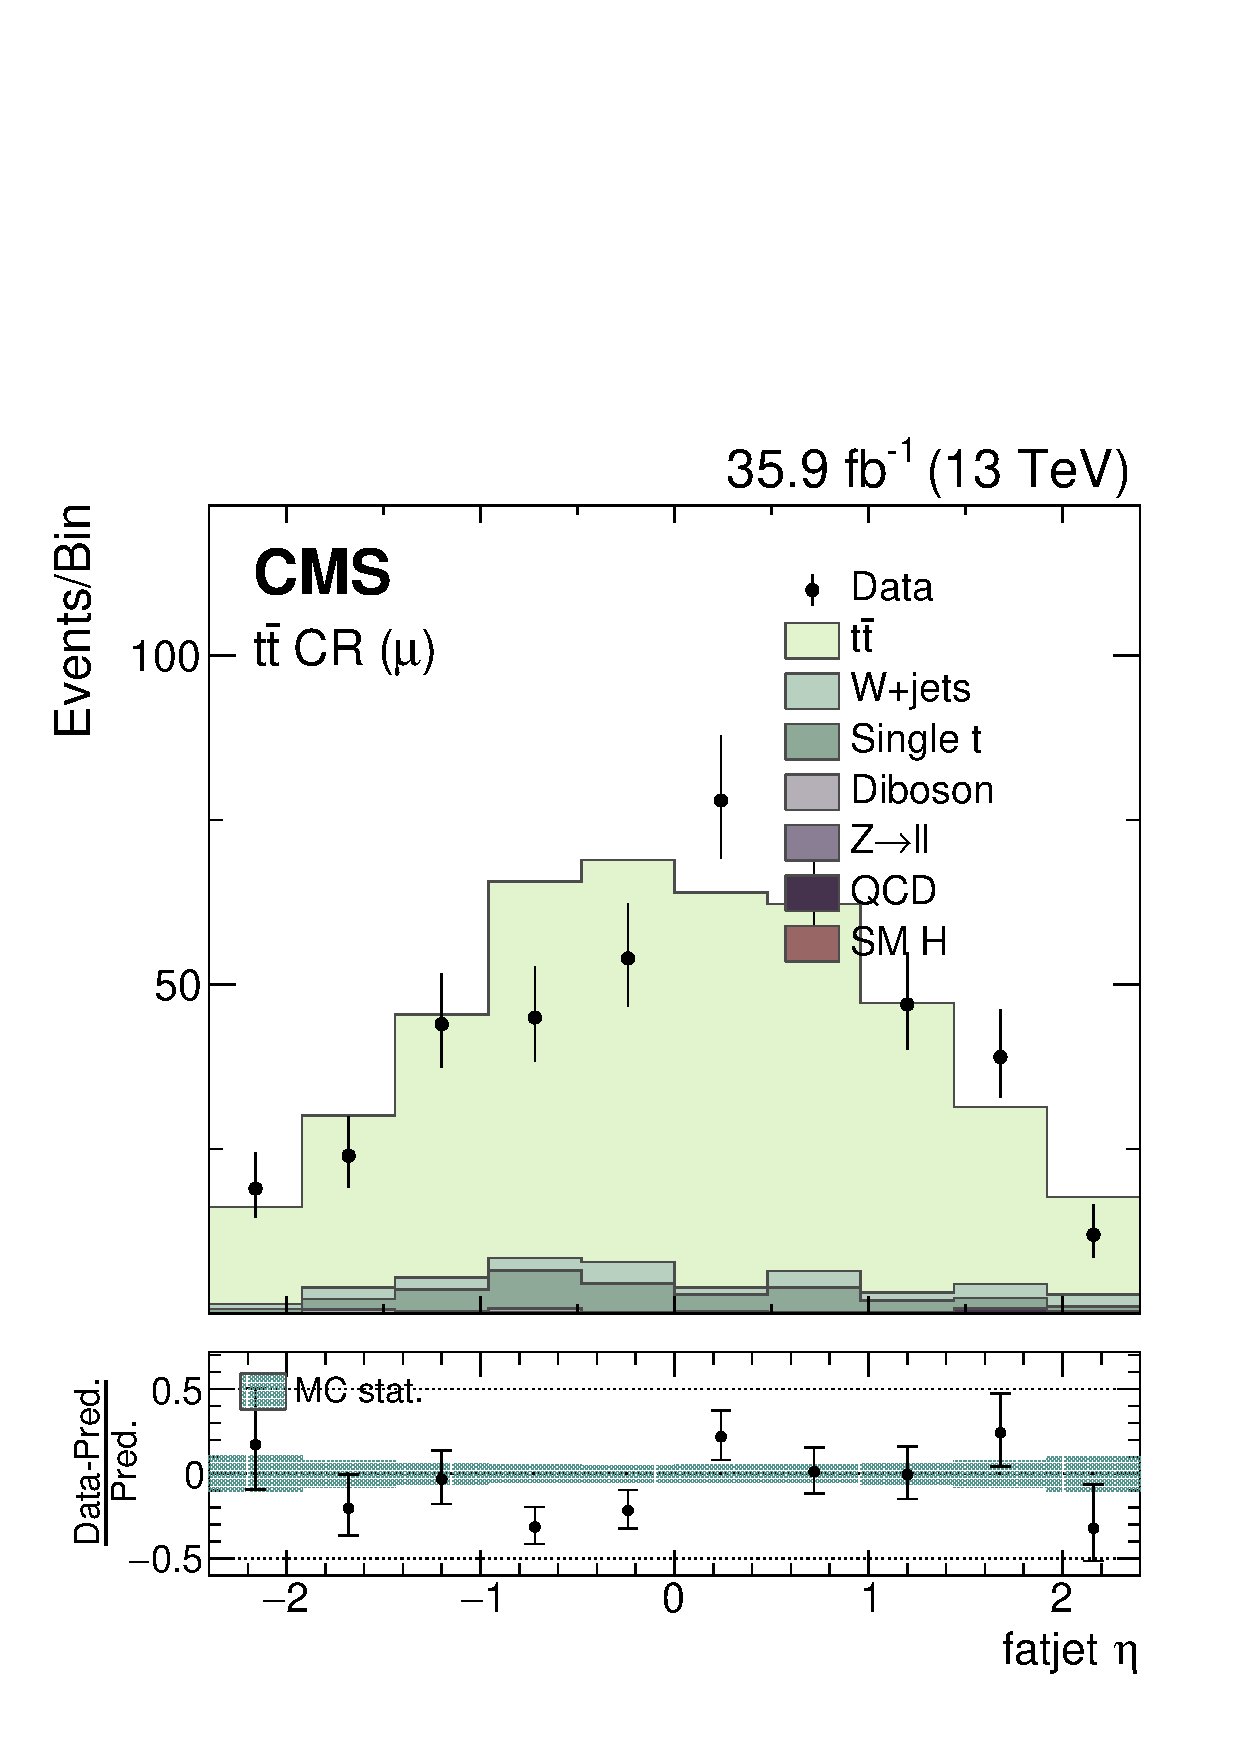
\includegraphics[width=0.4\textwidth]{figures/dataMC/cr_ttbar_mu_fj1Eta.pdf}} \\
 \subfloat{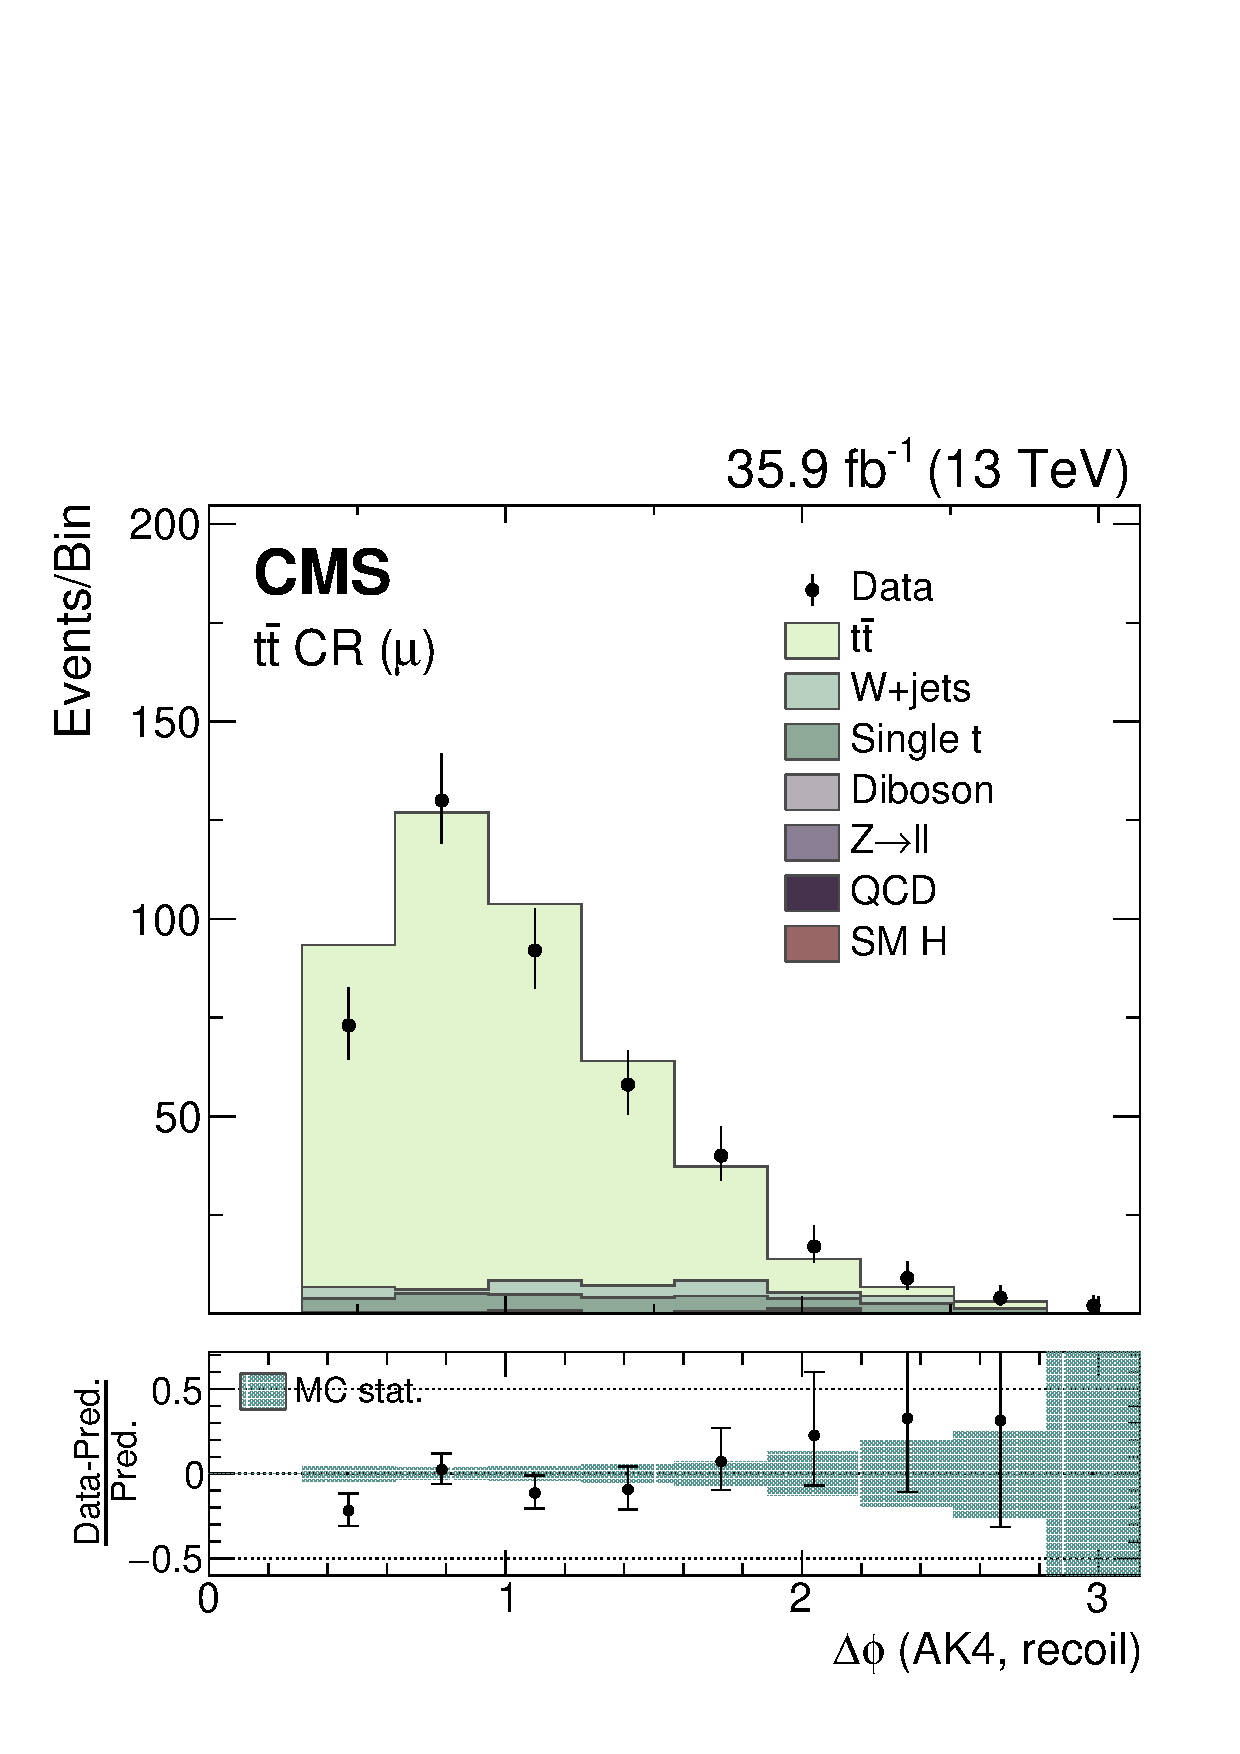
\includegraphics[width=0.4\textwidth]{figures/dataMC/cr_ttbar_mu_dphiUW.pdf}} 
 \subfloat{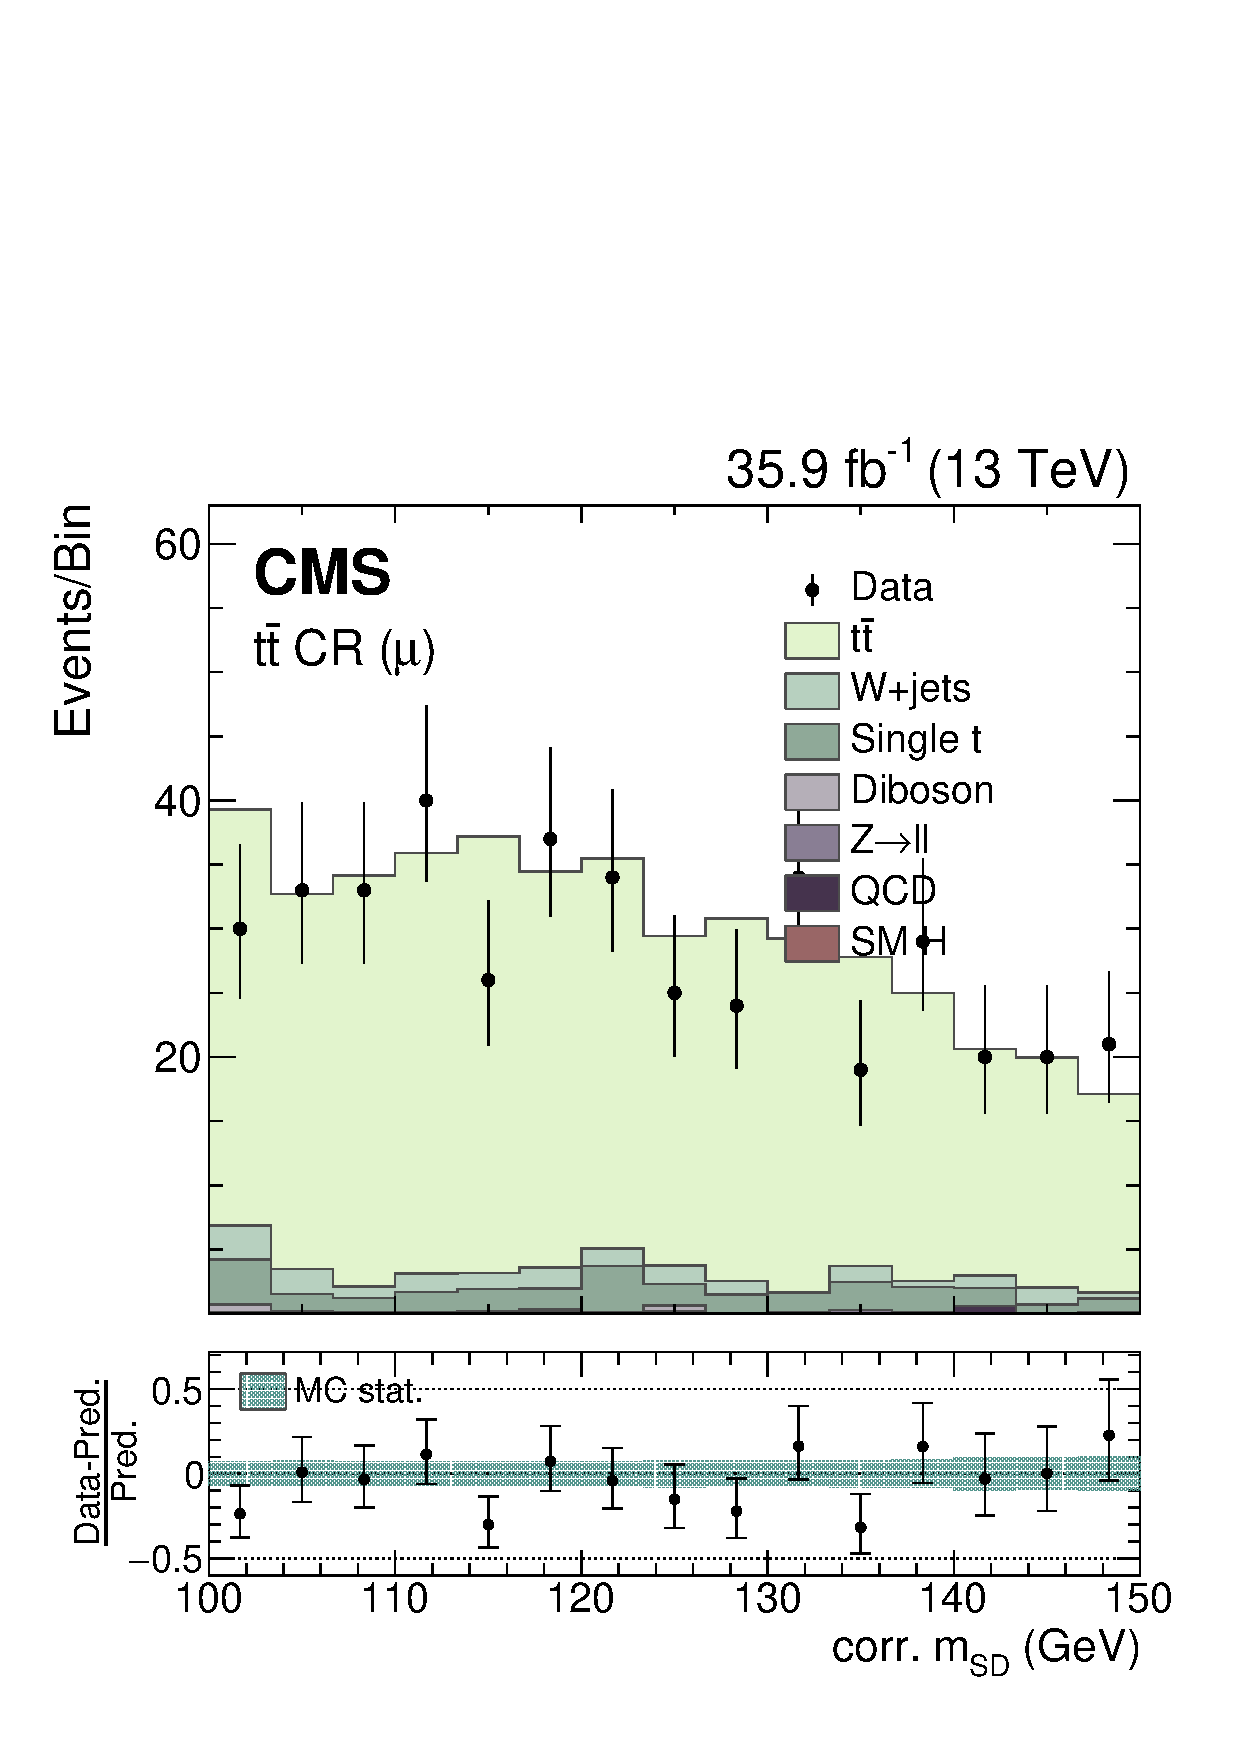
\includegraphics[width=0.4\textwidth]{figures/dataMC/cr_ttbar_mu_fj1MSD_corr.pdf}} \\
\caption{Prefit validation plots in the \ttbar CR (muon channel).}
\label{Fig_cr_ttbar_mu_1}
\end{figure}



\clearpage

\begin{figure}
\centering
 \subfloat{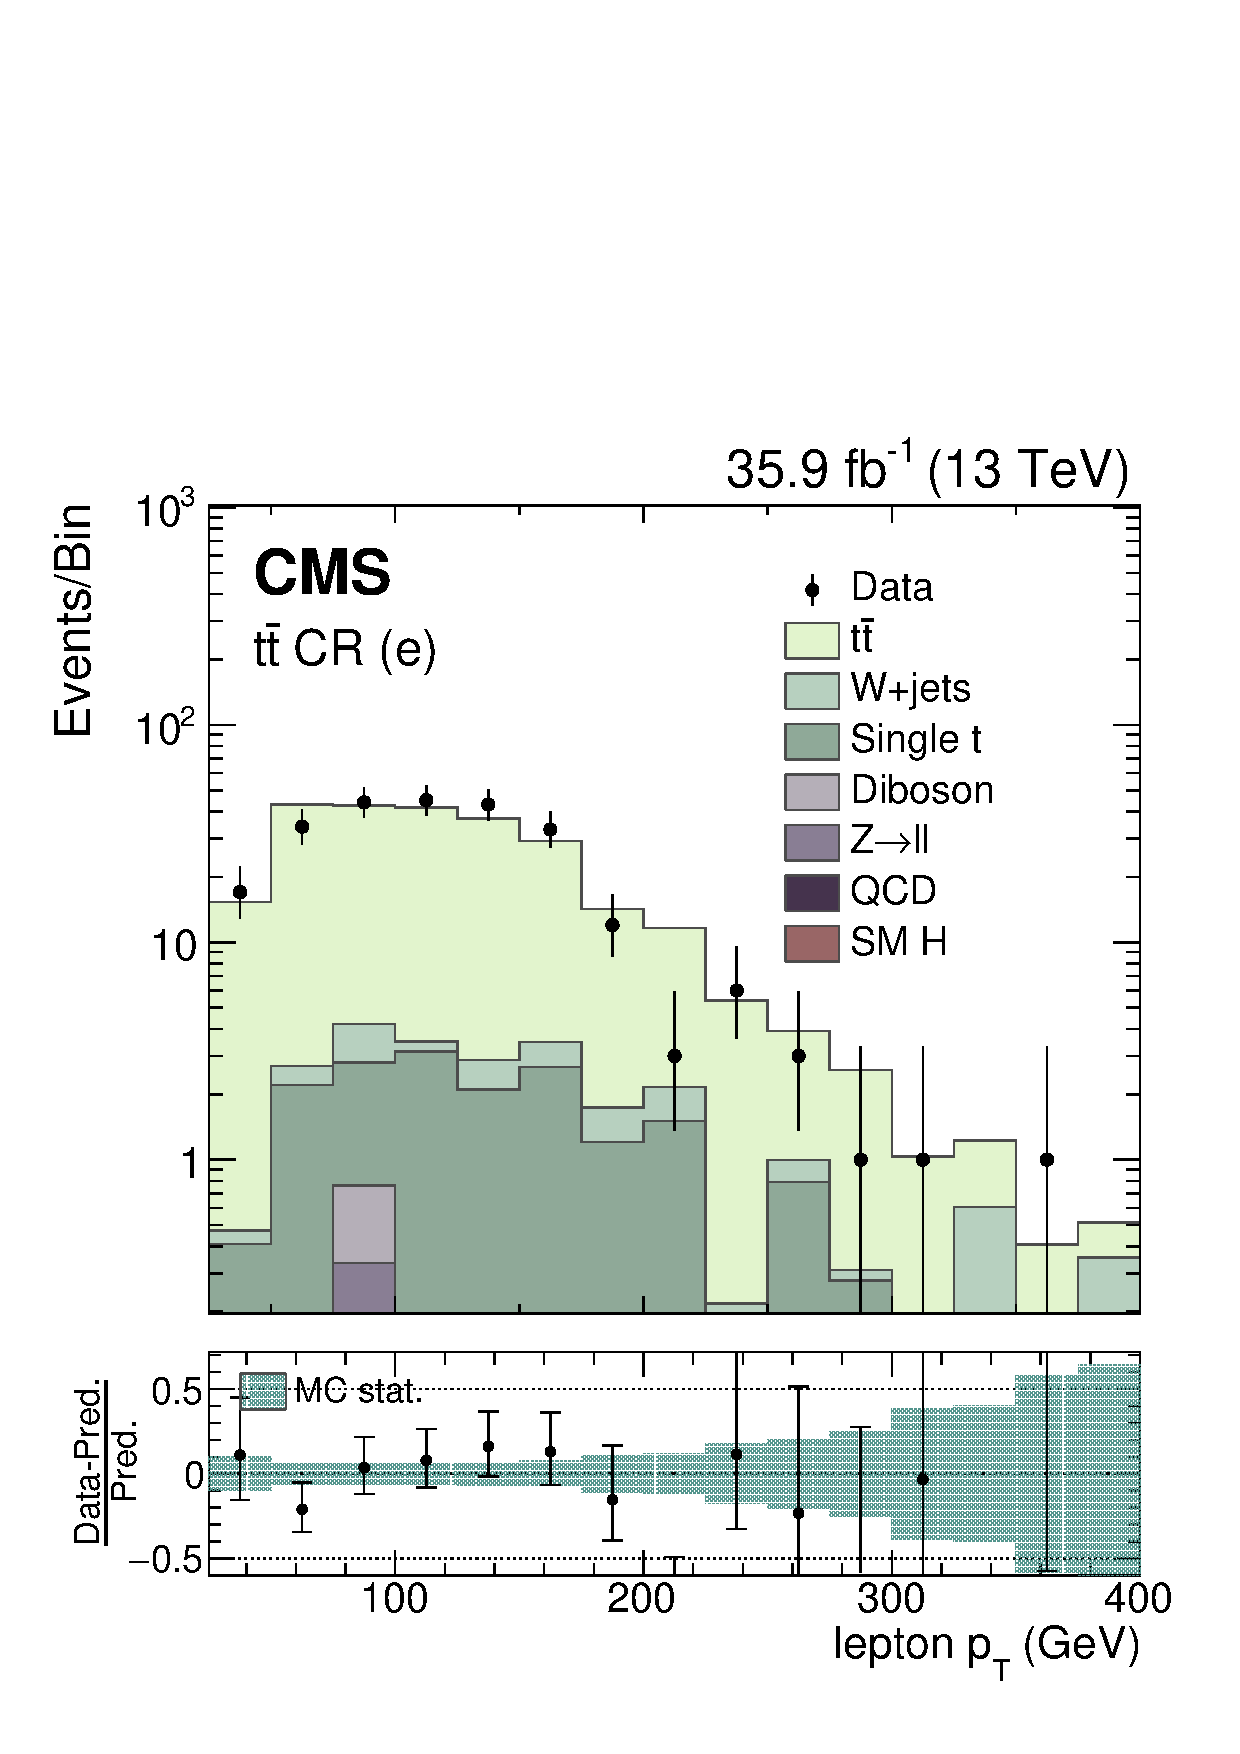
\includegraphics[width=0.4\textwidth]{figures/dataMC/cr_ttbar_el_lep1Pt.pdf}}
 \subfloat{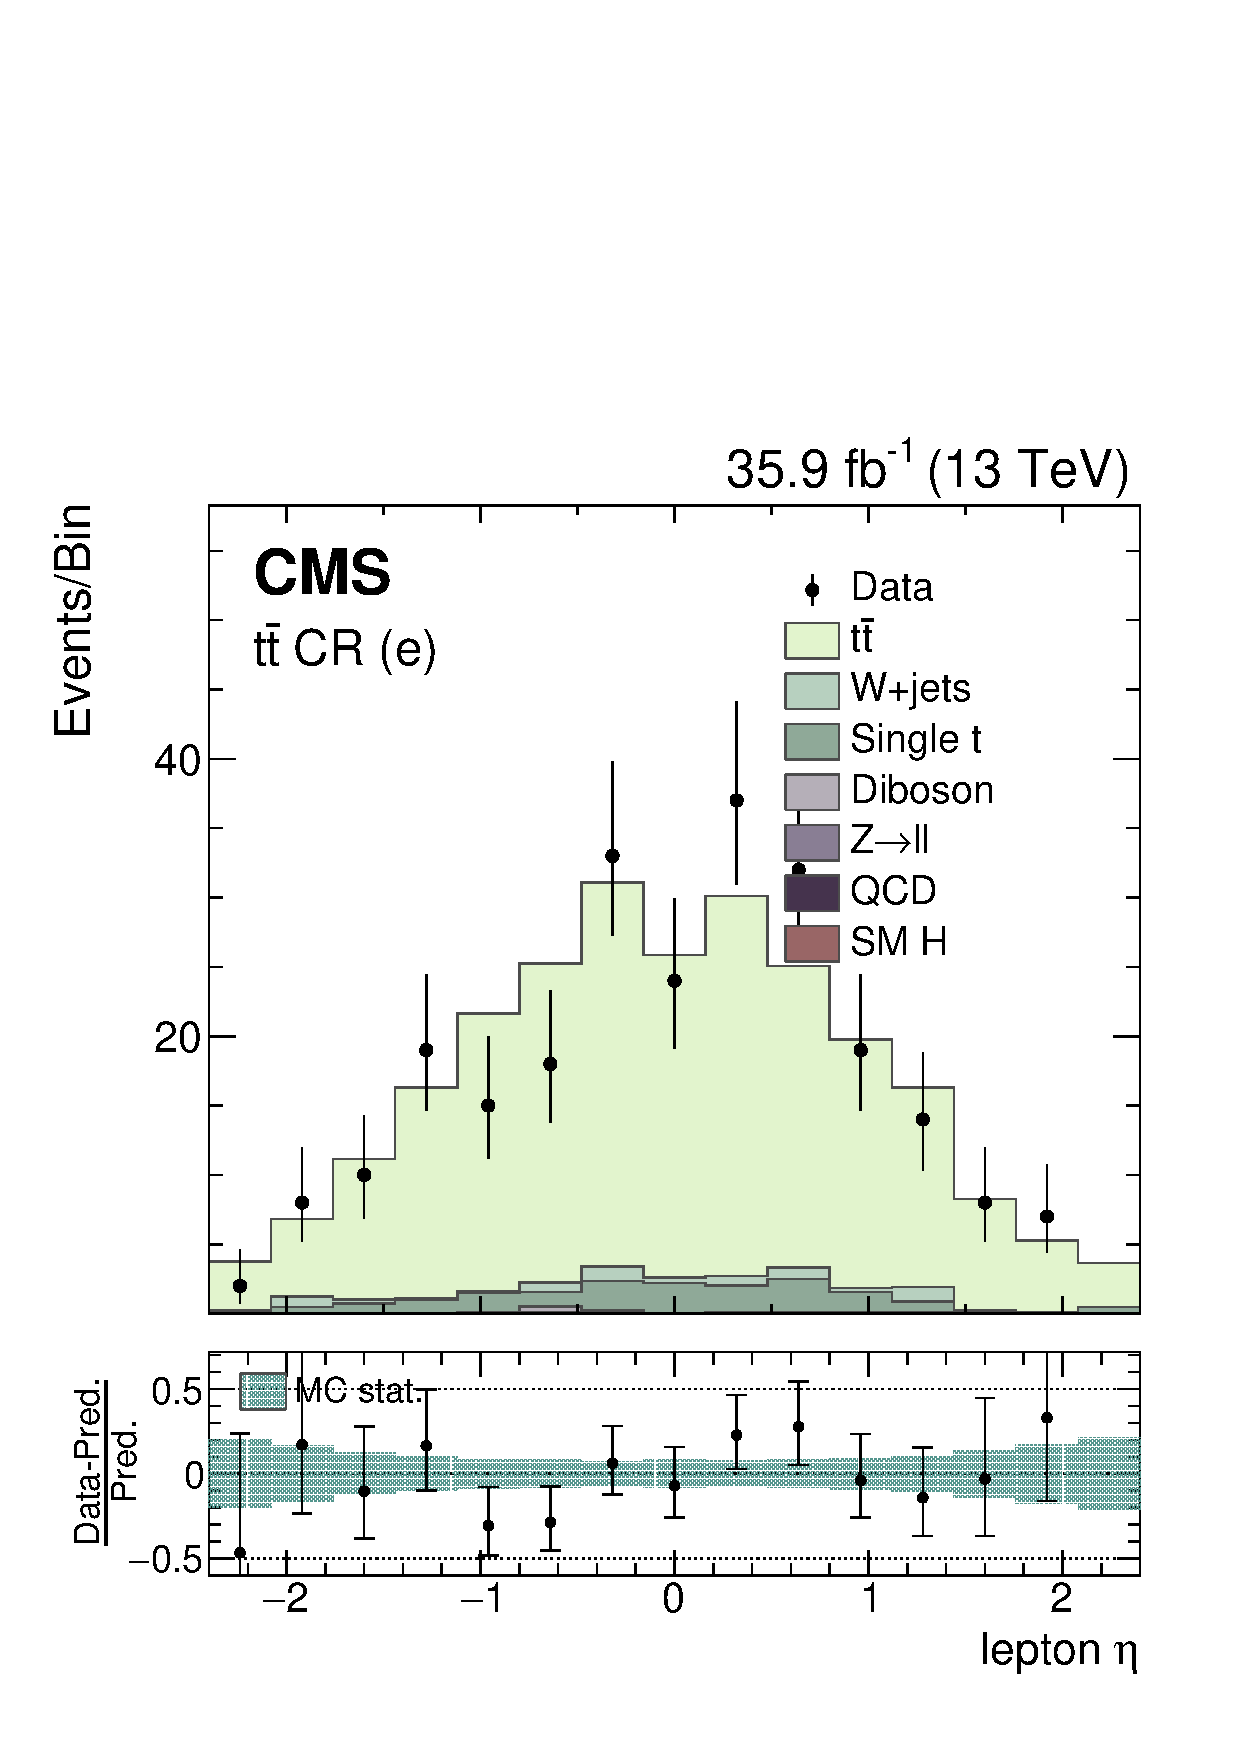
\includegraphics[width=0.4\textwidth]{figures/dataMC/cr_ttbar_el_lep1Eta.pdf}} \\
 \subfloat{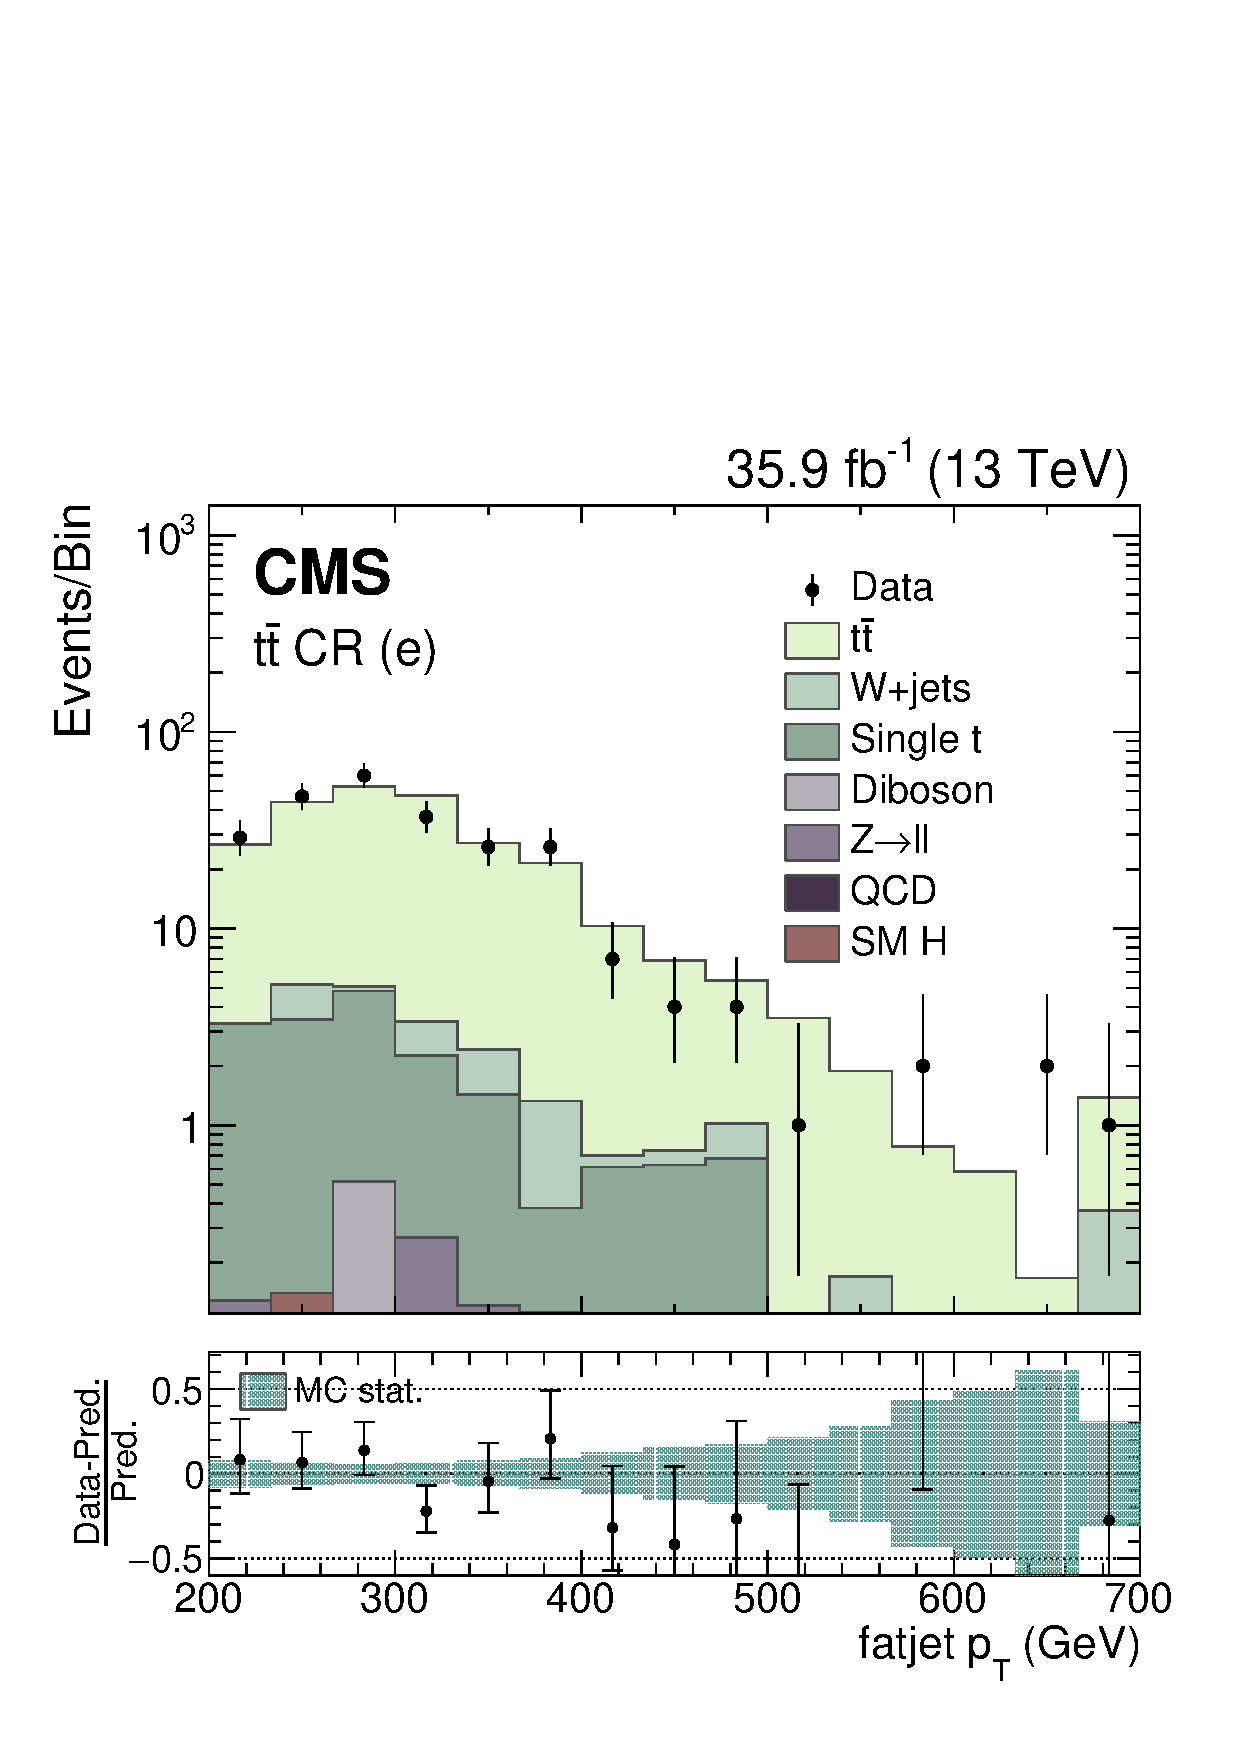
\includegraphics[width=0.4\textwidth]{figures/dataMC/cr_ttbar_el_fj1Pt.pdf}}
 \subfloat{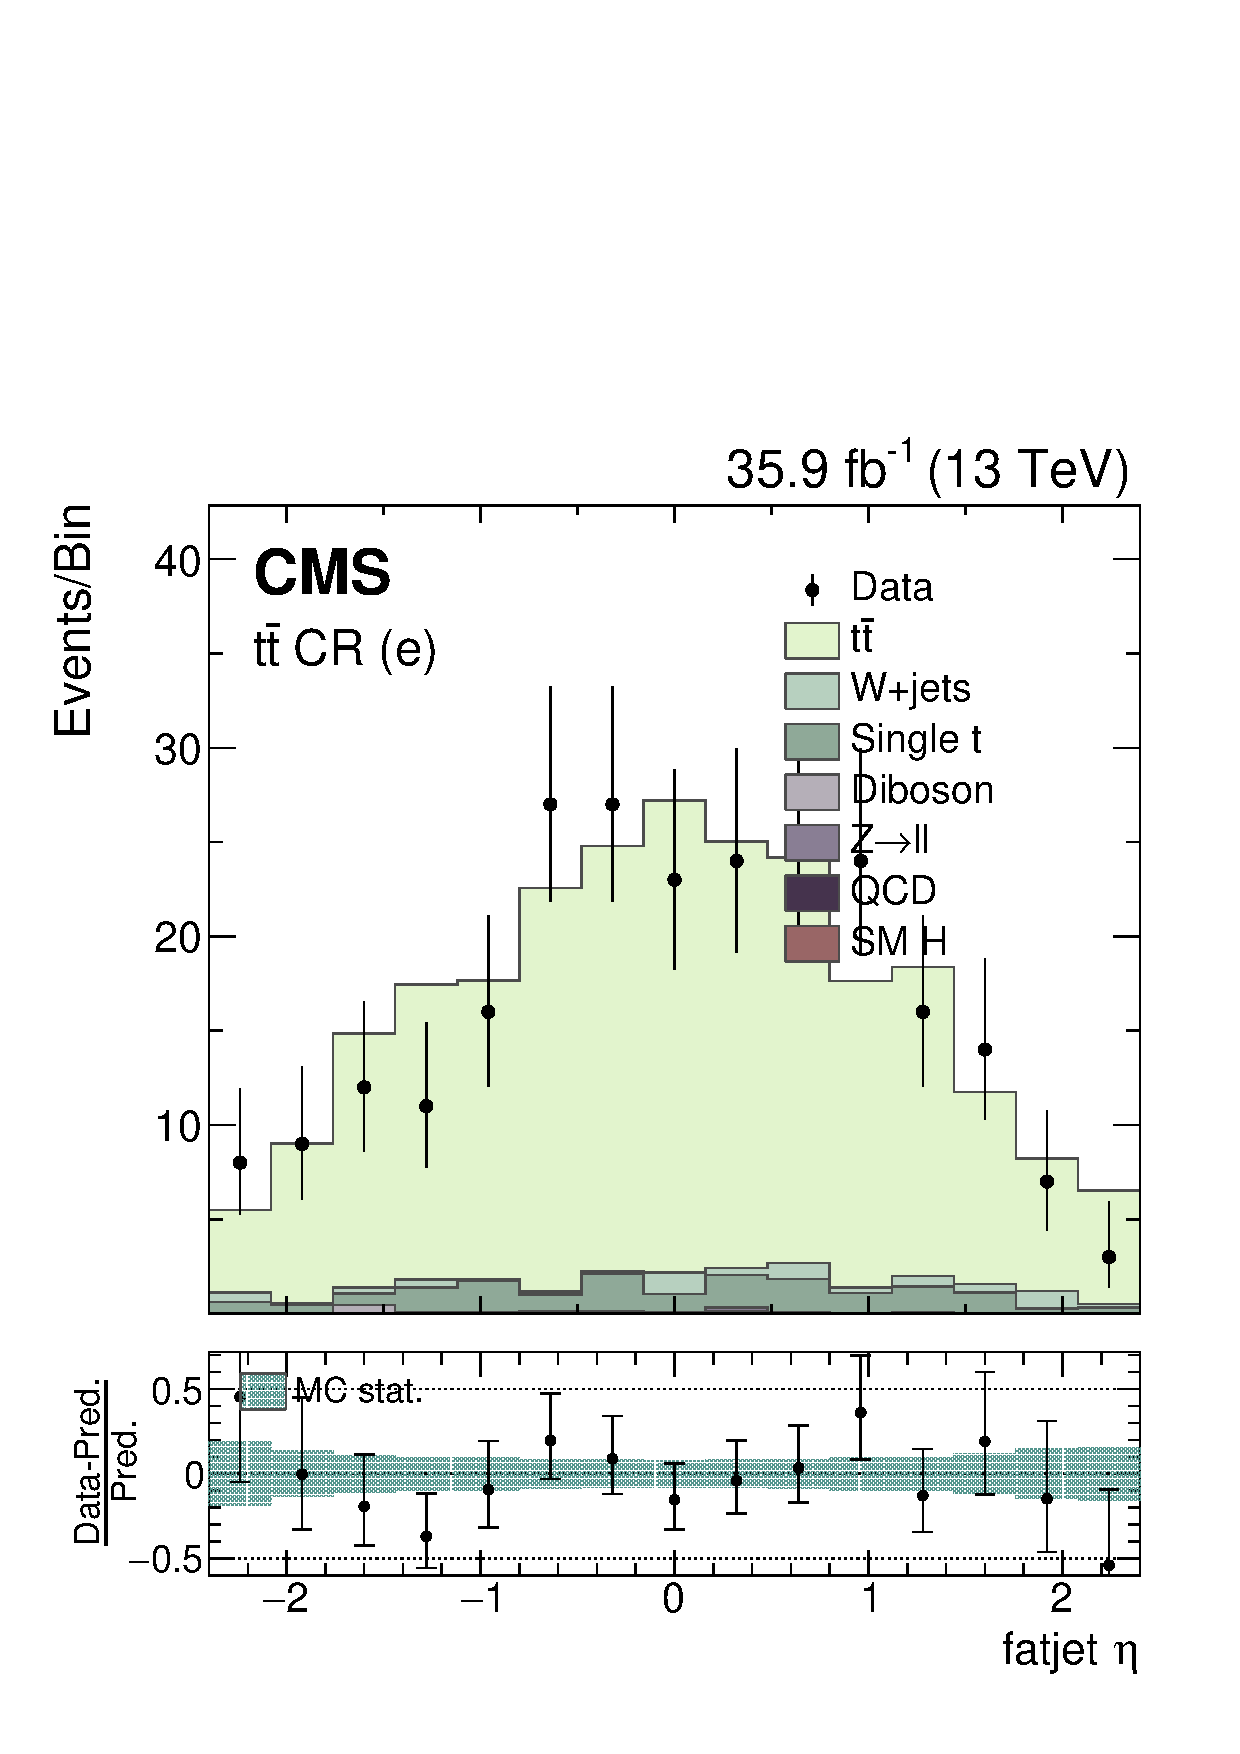
\includegraphics[width=0.4\textwidth]{figures/dataMC/cr_ttbar_el_fj1Eta.pdf}} \\
 \subfloat{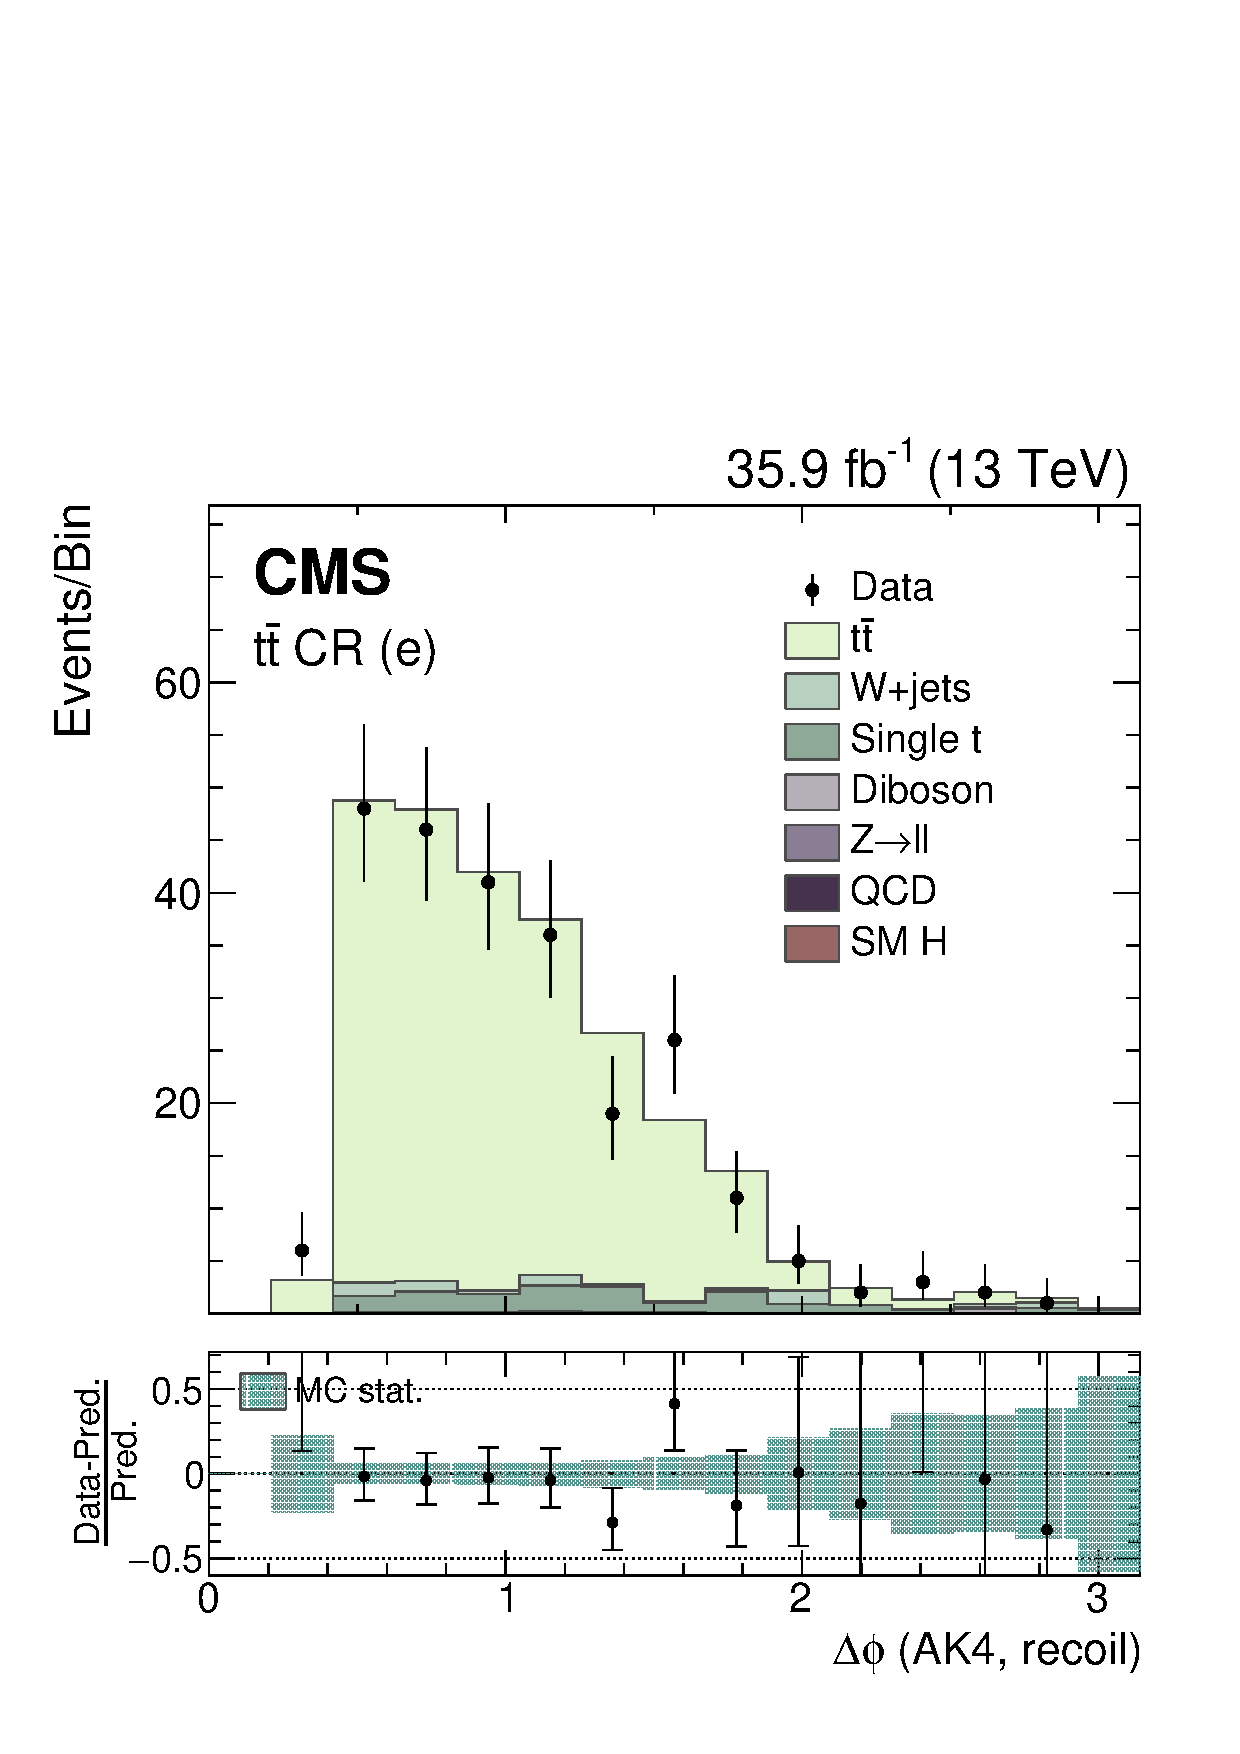
\includegraphics[width=0.4\textwidth]{figures/dataMC/cr_ttbar_el_dphiUW.pdf}} 
 \subfloat{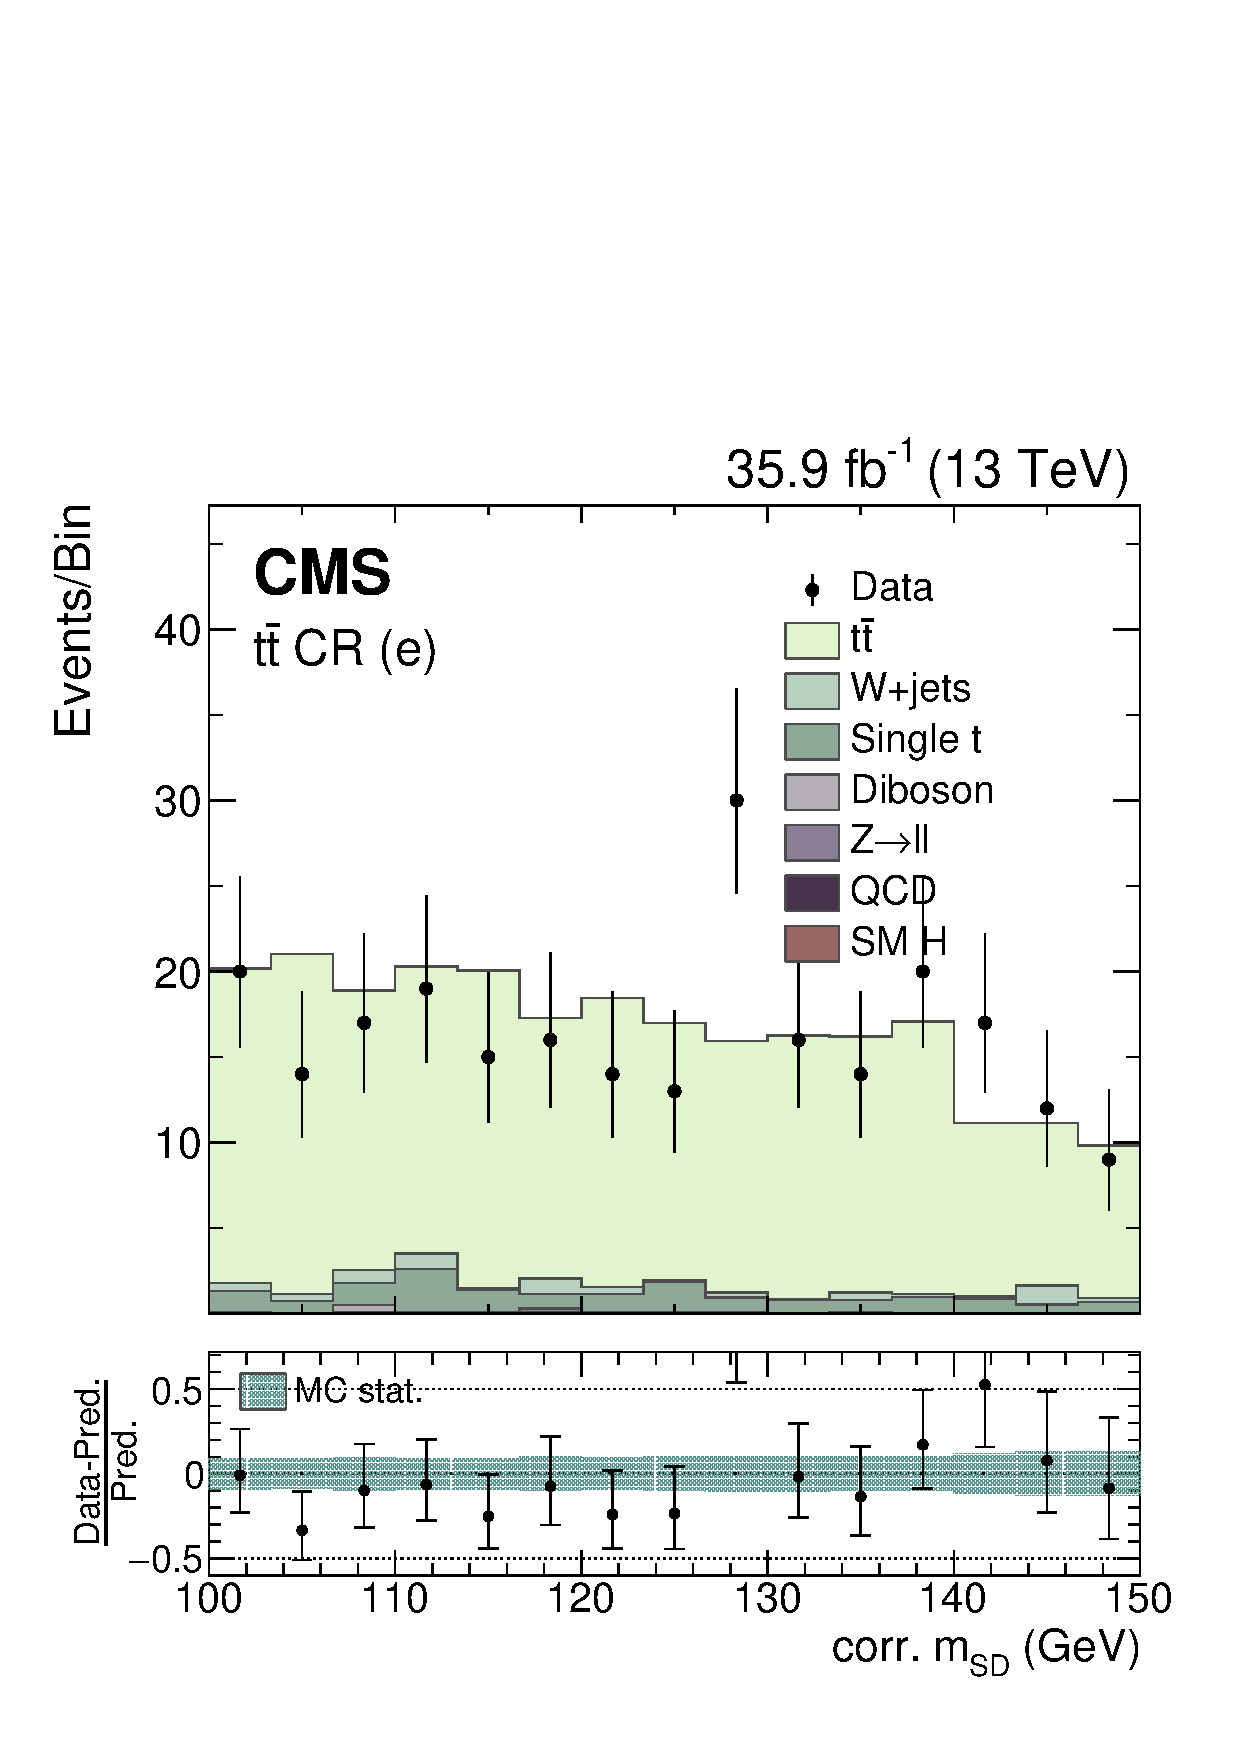
\includegraphics[width=0.4\textwidth]{figures/dataMC/cr_ttbar_el_fj1MSD_corr.pdf}} \\
\caption{Prefit validation plots in the \ttbar CR (electron channel).}
\label{Fig_cr_ttbar_el_1}
\end{figure}


\clearpage

\begin{figure}
\centering
 \subfloat{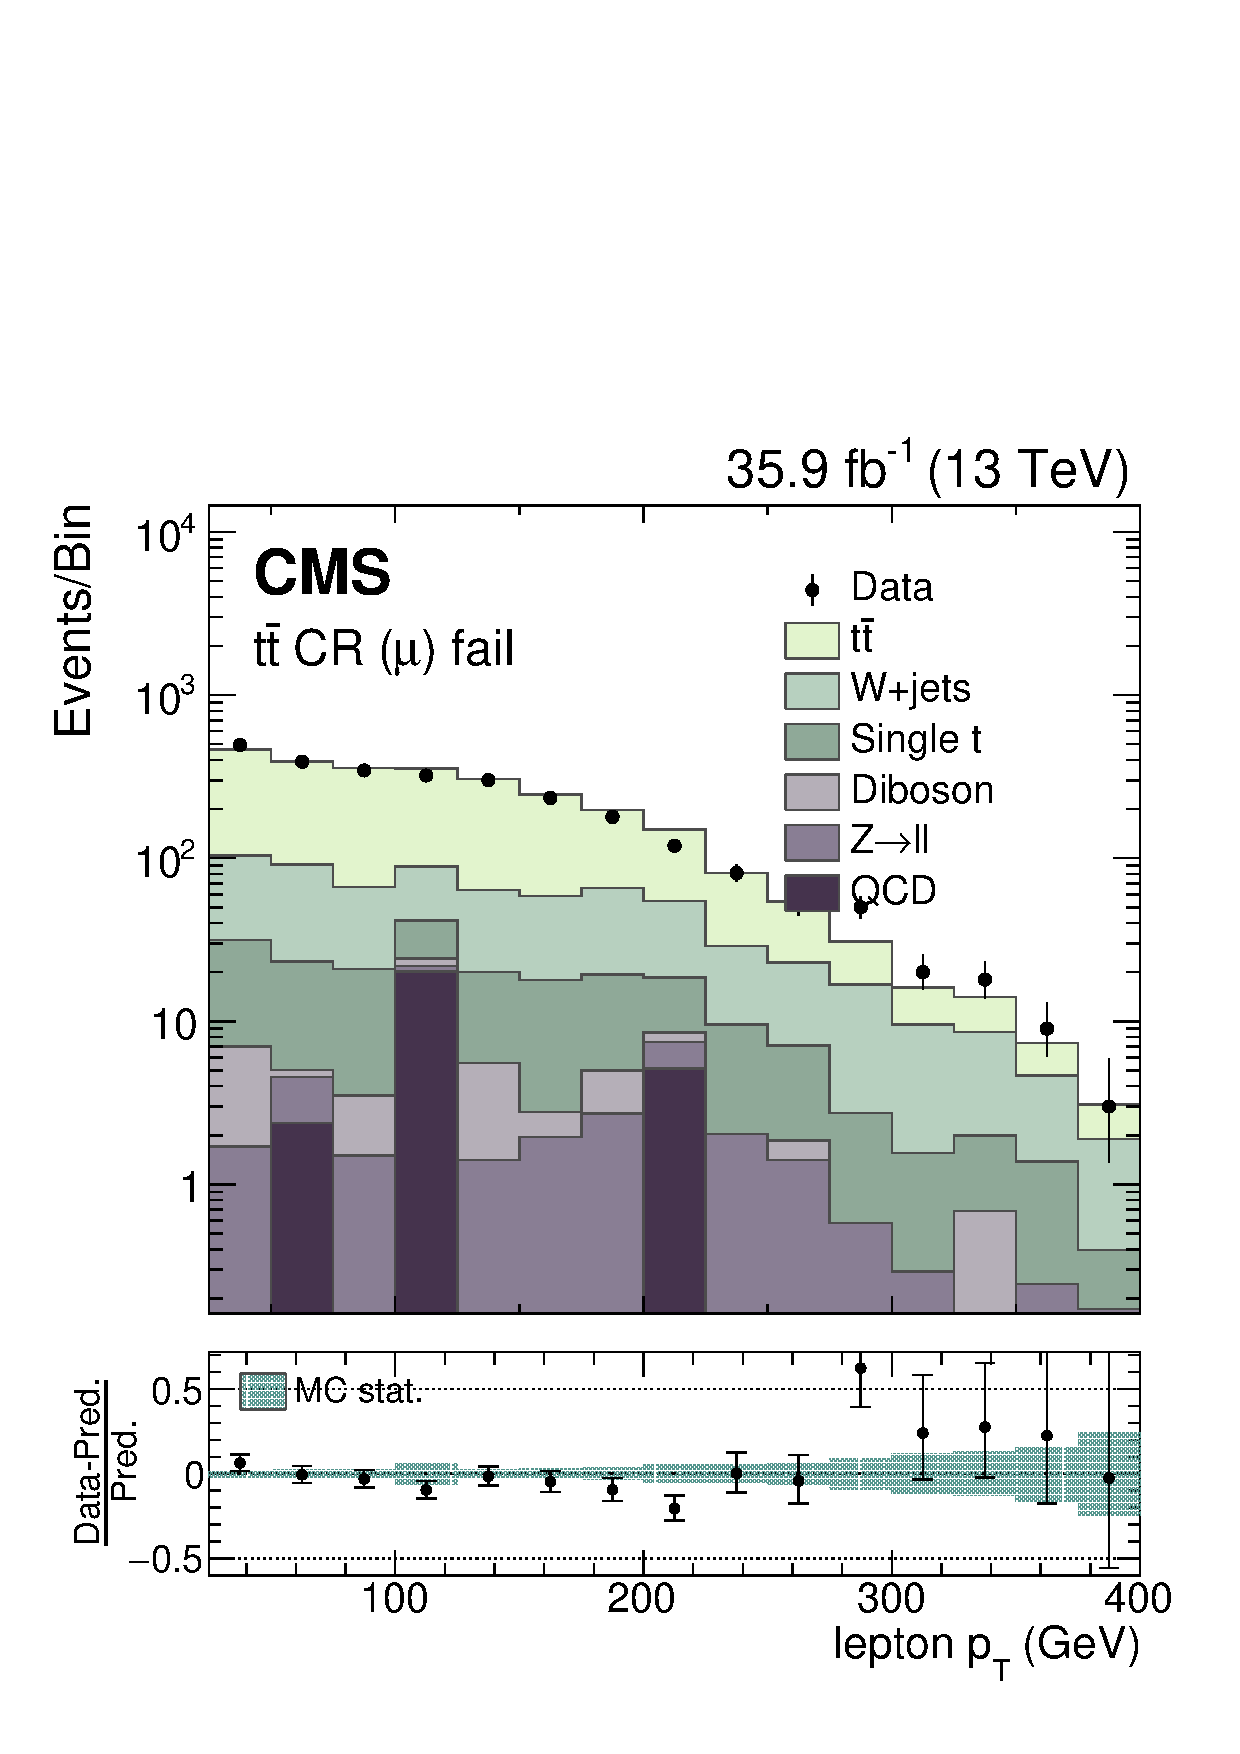
\includegraphics[width=0.4\textwidth]{figures/dataMC/cr_ttbar_mu_fail_lep1Pt.pdf}}
 \subfloat{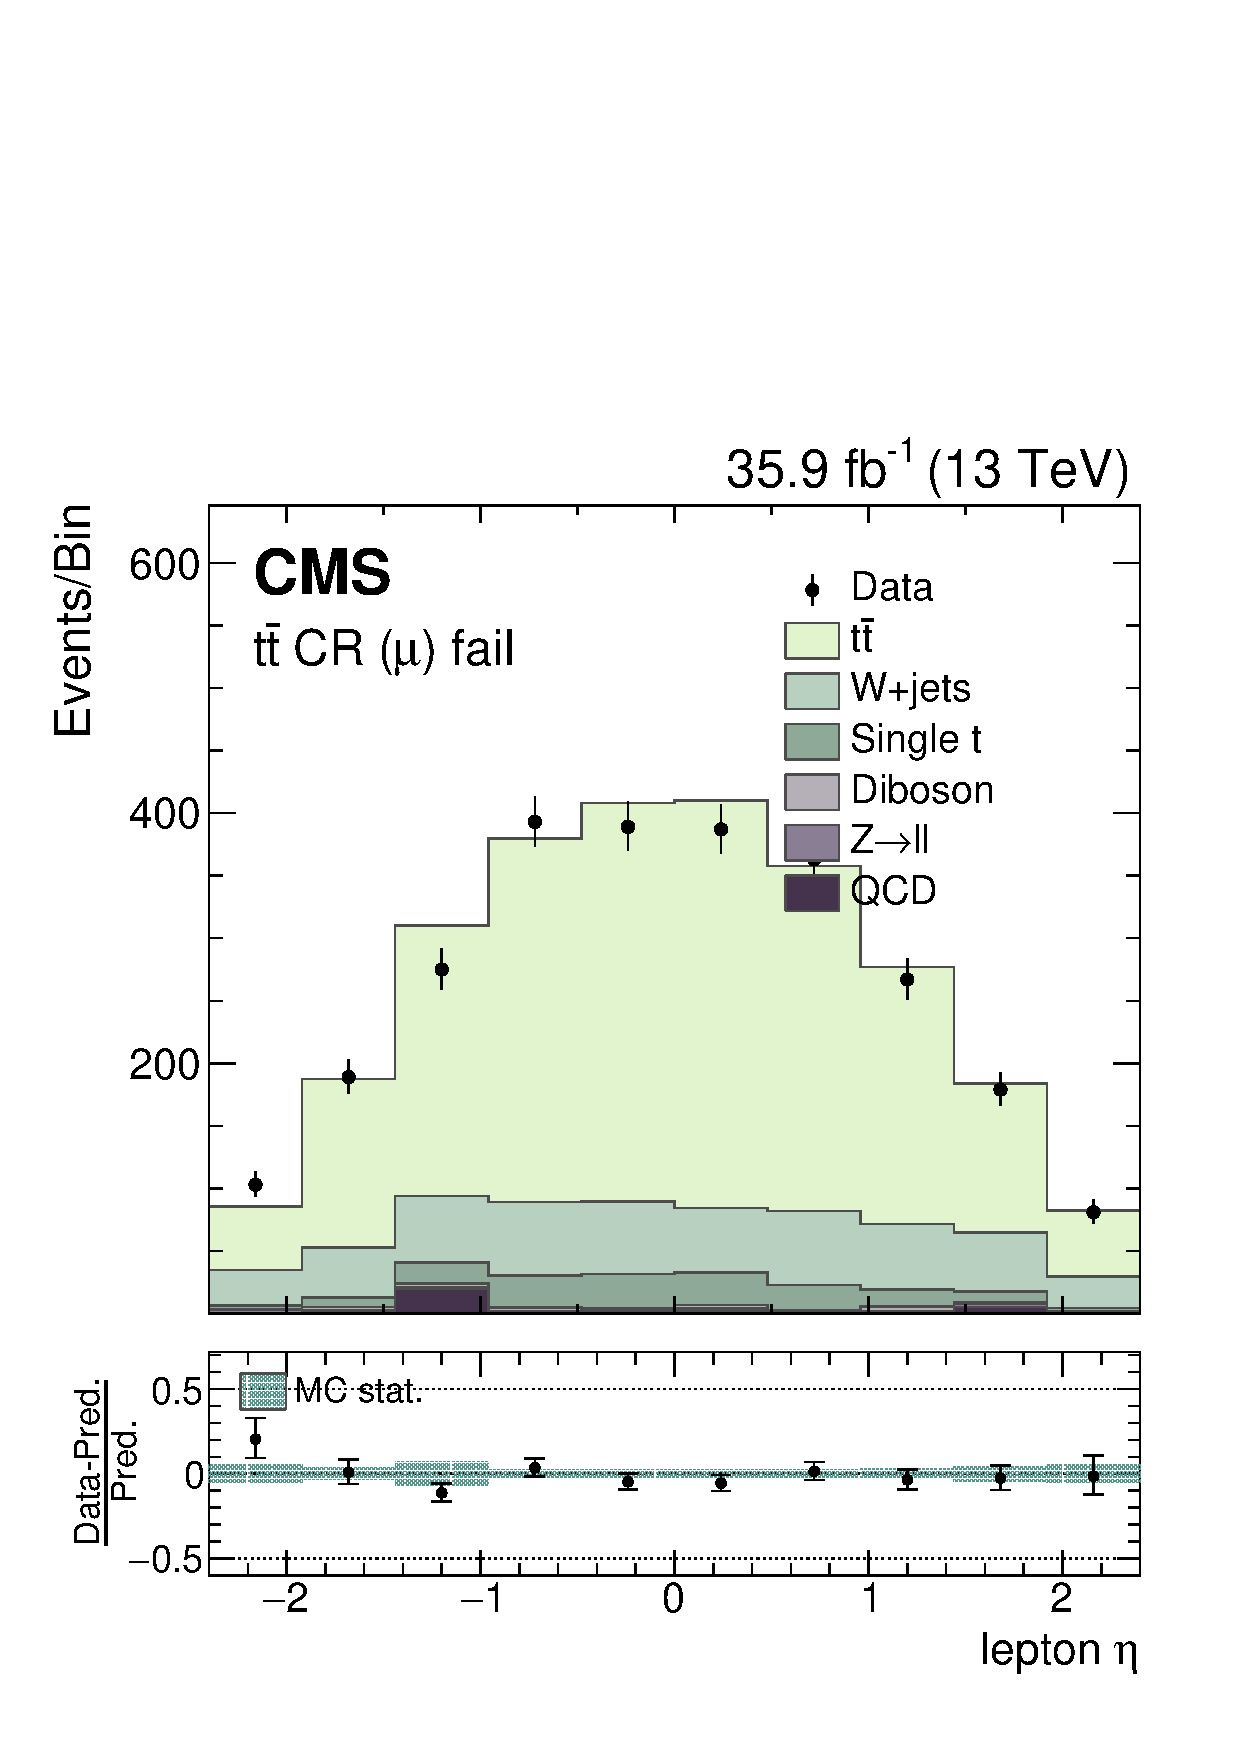
\includegraphics[width=0.4\textwidth]{figures/dataMC/cr_ttbar_mu_fail_lep1Eta.pdf}} \\
 \subfloat{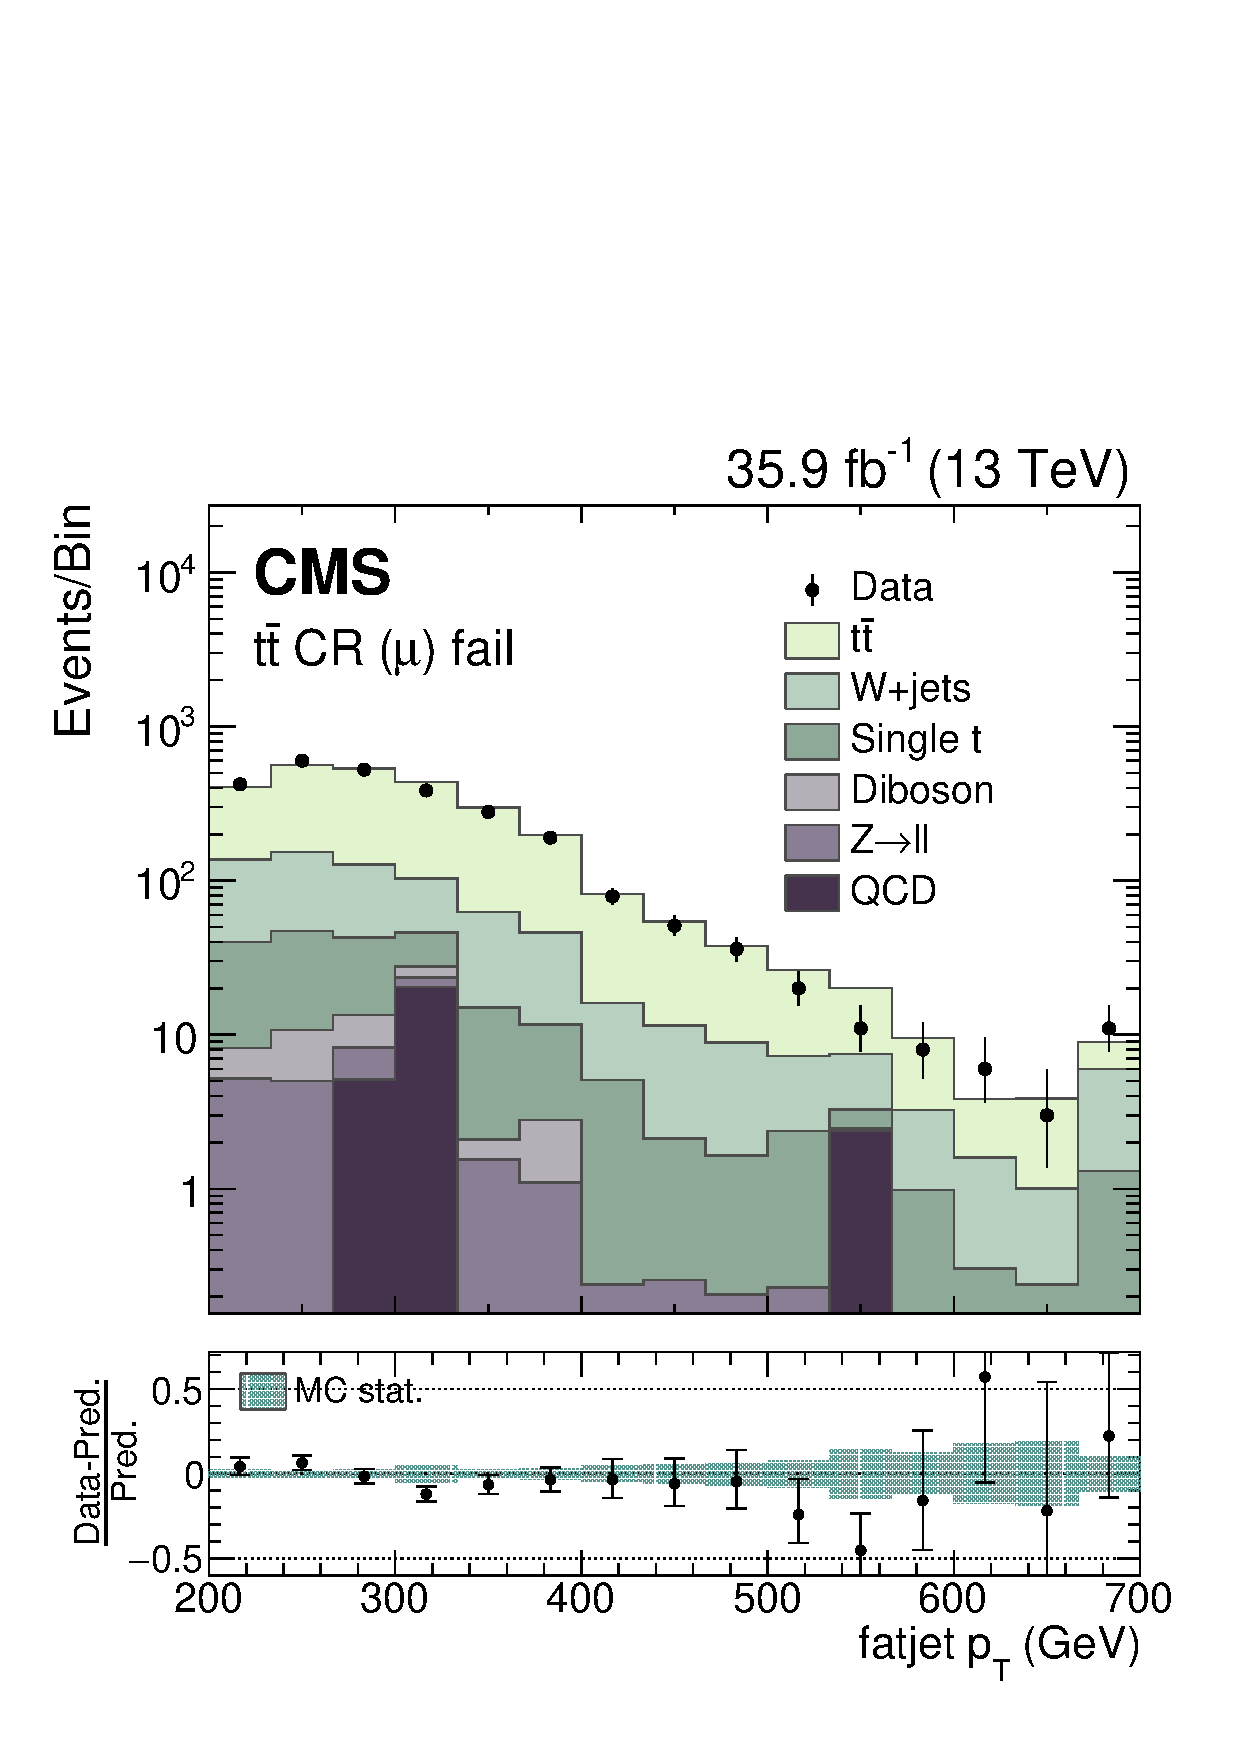
\includegraphics[width=0.4\textwidth]{figures/dataMC/cr_ttbar_mu_fail_fj1Pt.pdf}}
 \subfloat{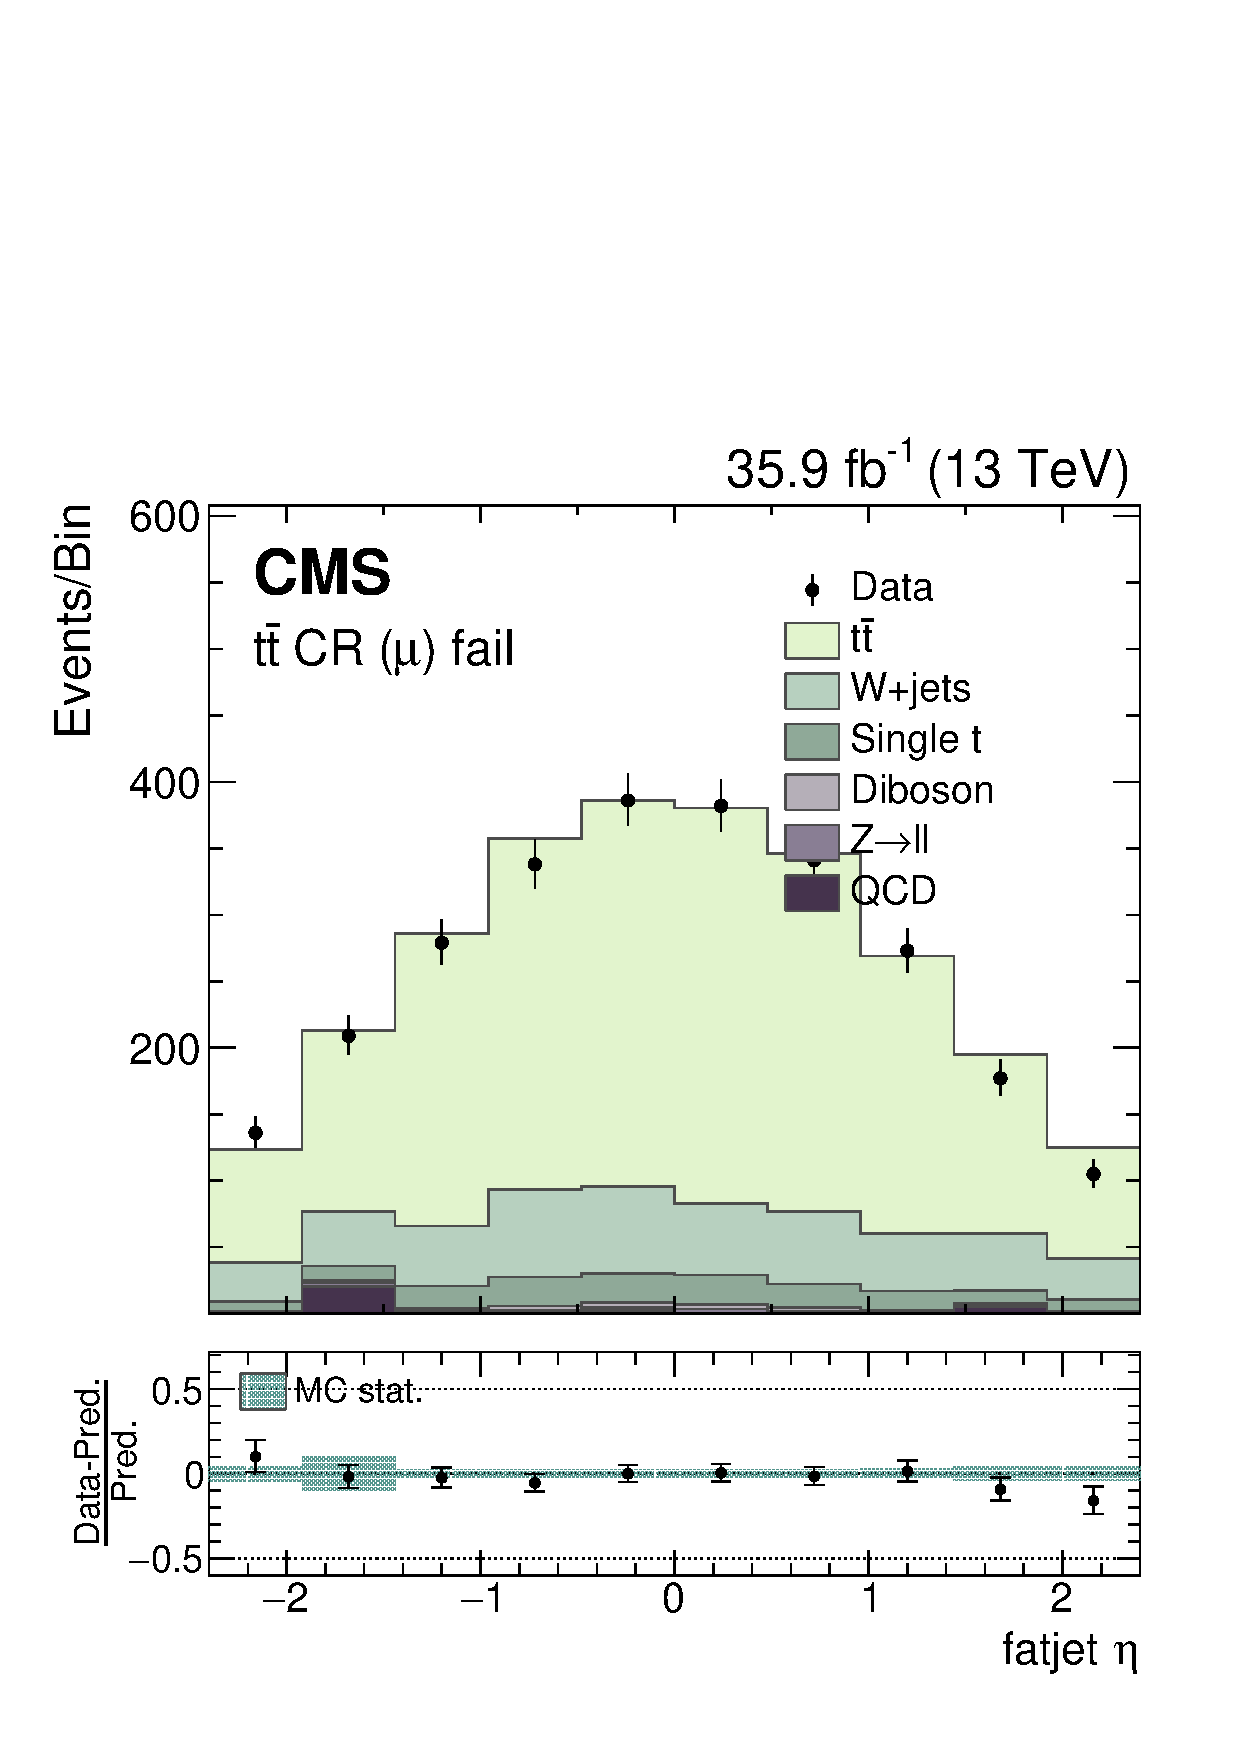
\includegraphics[width=0.4\textwidth]{figures/dataMC/cr_ttbar_mu_fail_fj1Eta.pdf}} \\
 \subfloat{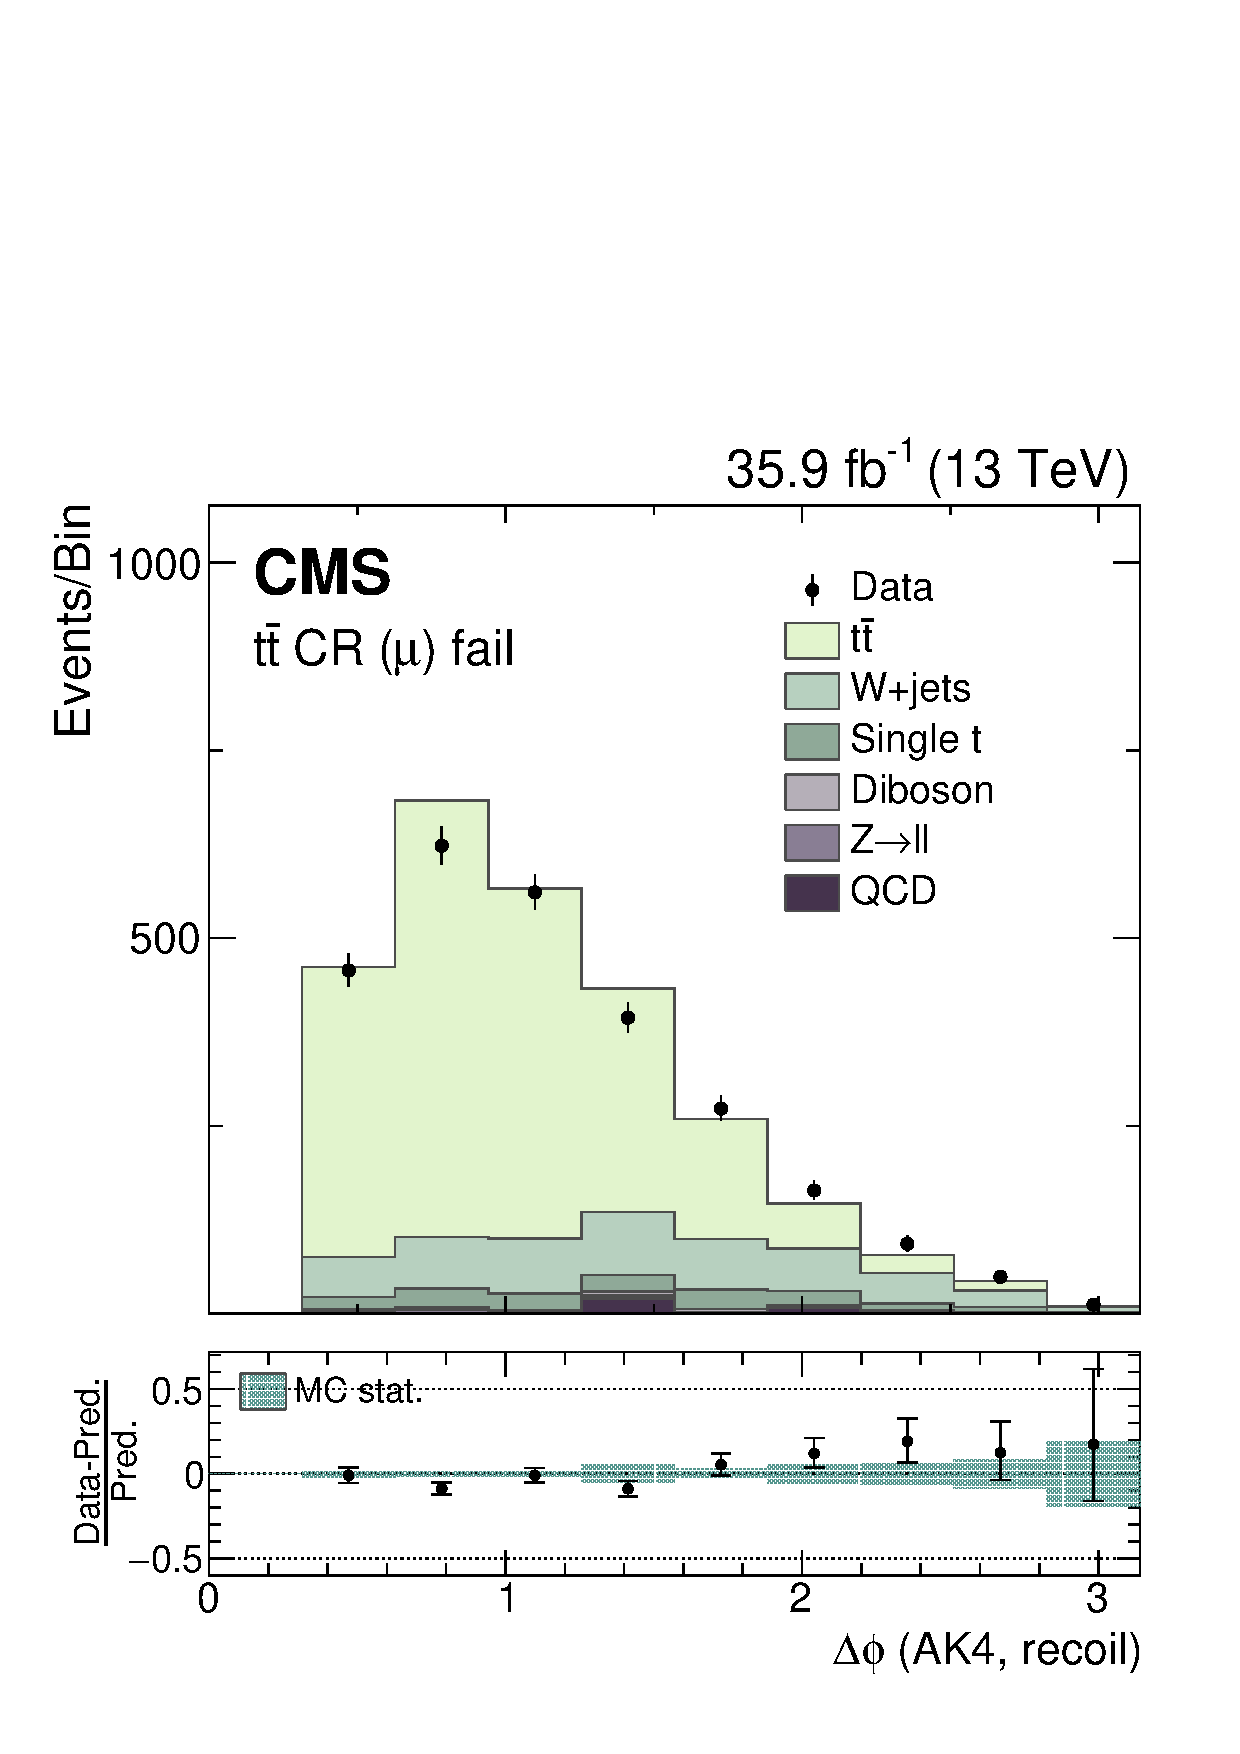
\includegraphics[width=0.4\textwidth]{figures/dataMC/cr_ttbar_mu_fail_dphiUW.pdf}} 
 \subfloat{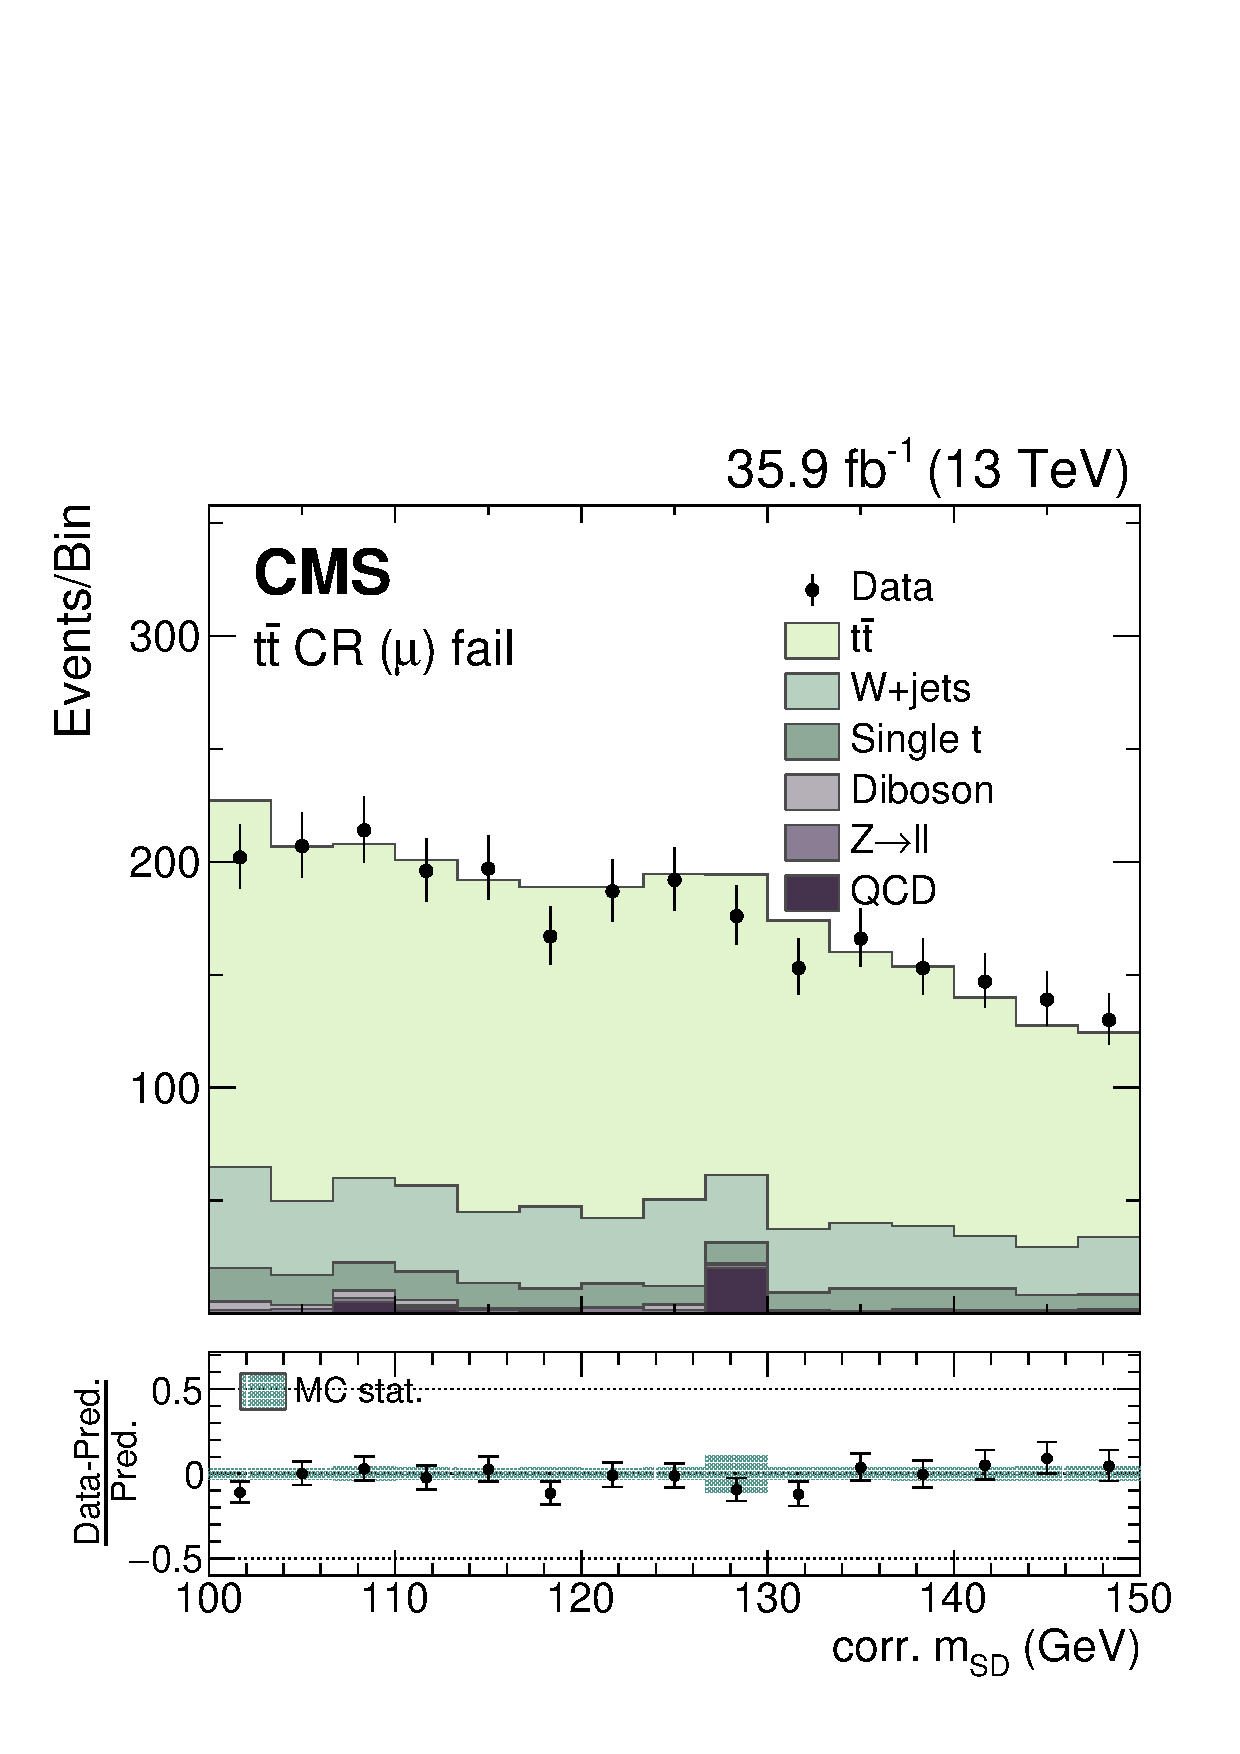
\includegraphics[width=0.4\textwidth]{figures/dataMC/cr_ttbar_mu_fail_fj1MSD_corr.pdf}} \\
\caption{Prefit validation plots in the \ttbar fail CR (muon channel).}
\label{Fig_cr_ttbar_mu_1}
\end{figure}



\clearpage

\begin{figure}
\centering
 \subfloat{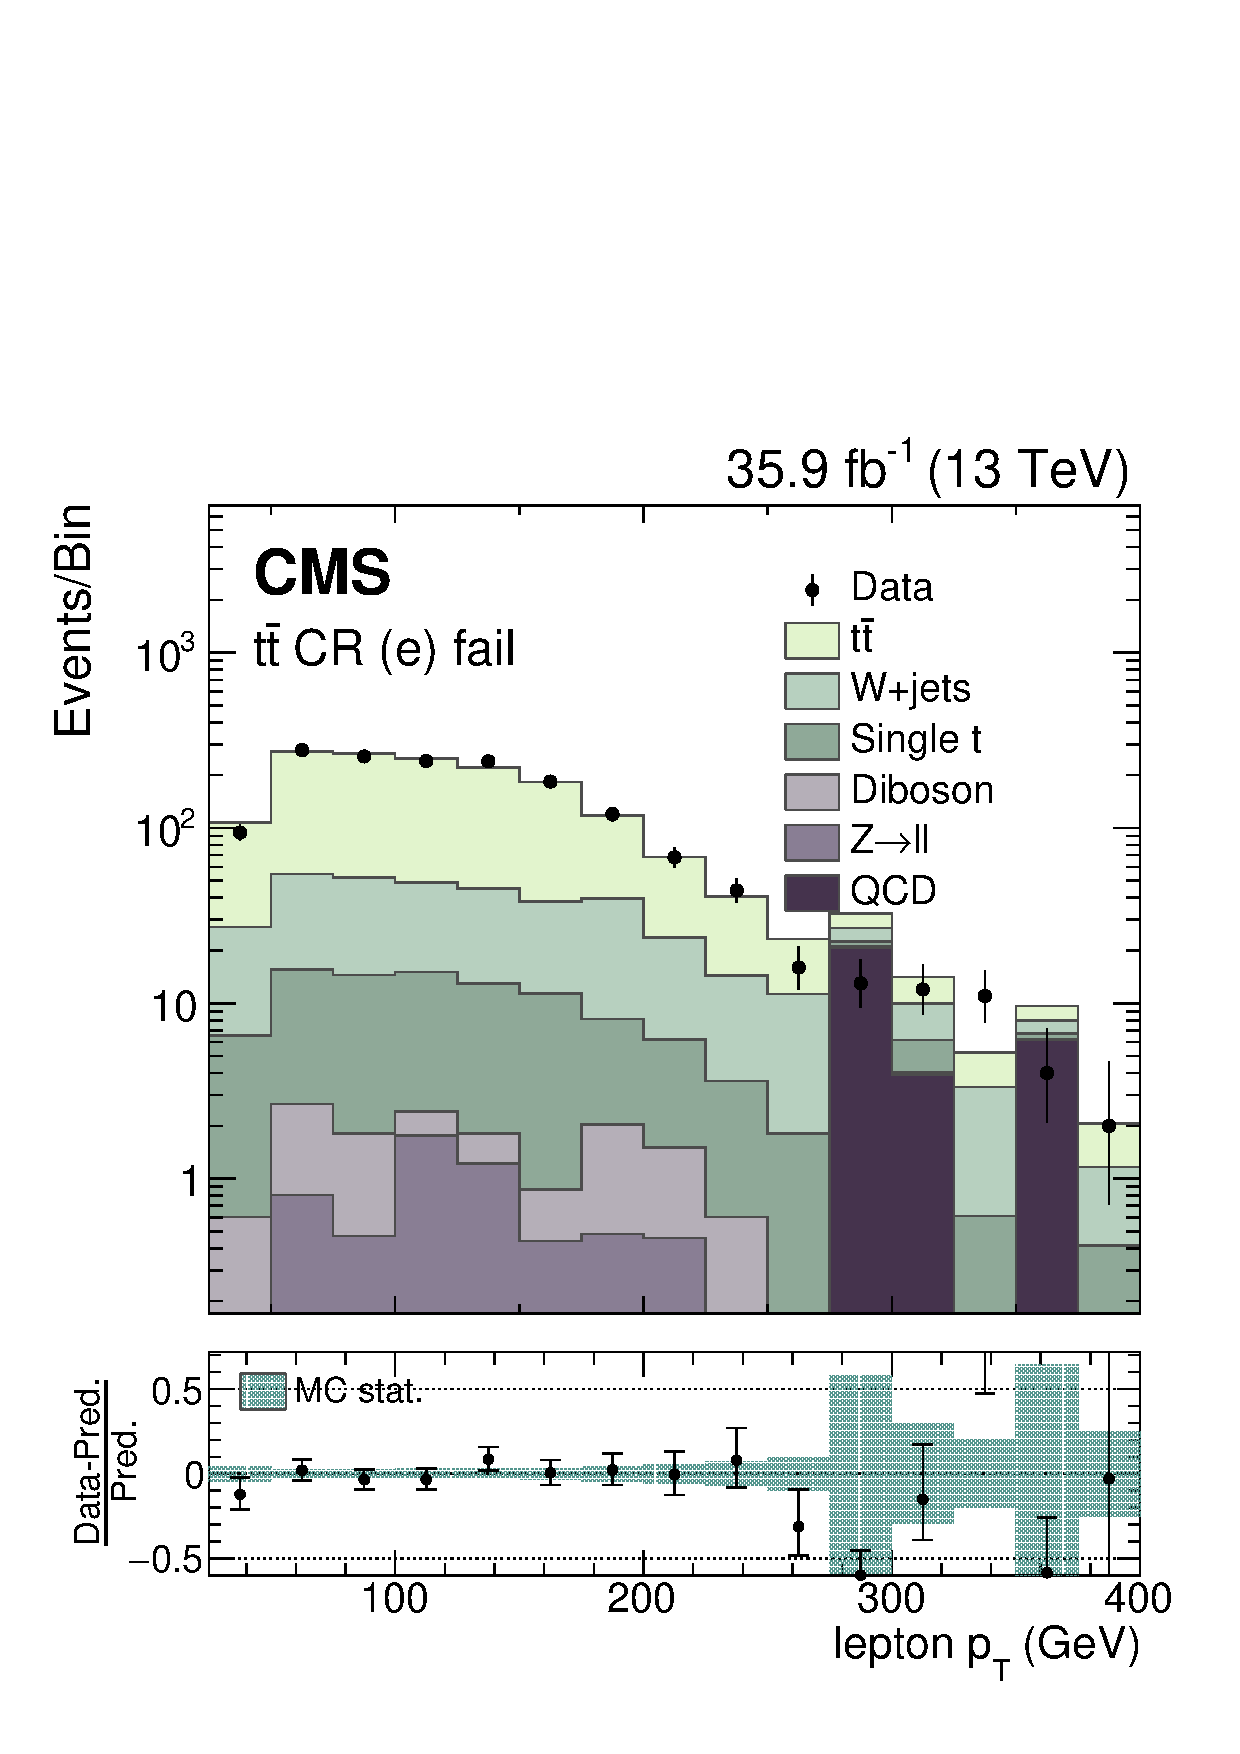
\includegraphics[width=0.4\textwidth]{figures/dataMC/cr_ttbar_el_fail_lep1Pt.pdf}}
 \subfloat{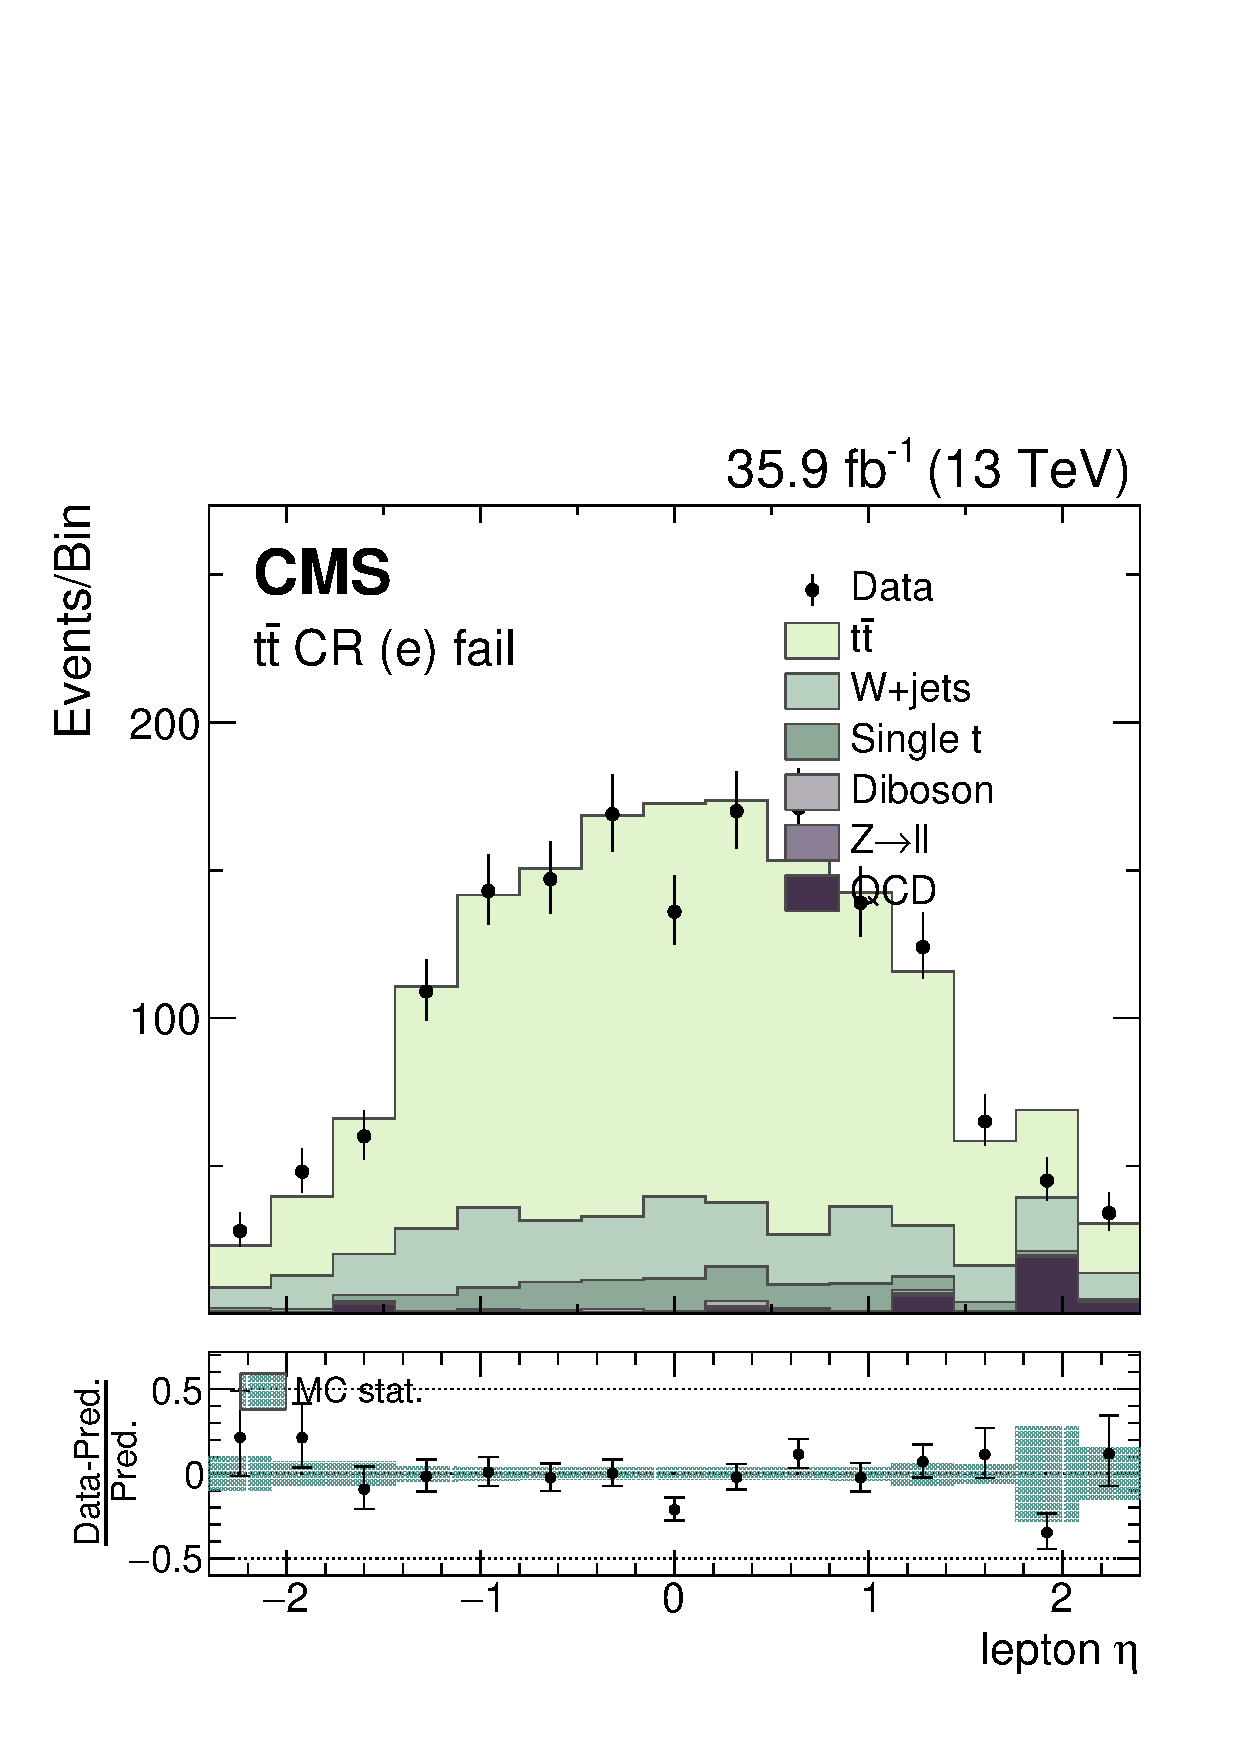
\includegraphics[width=0.4\textwidth]{figures/dataMC/cr_ttbar_el_fail_lep1Eta.pdf}} \\
 \subfloat{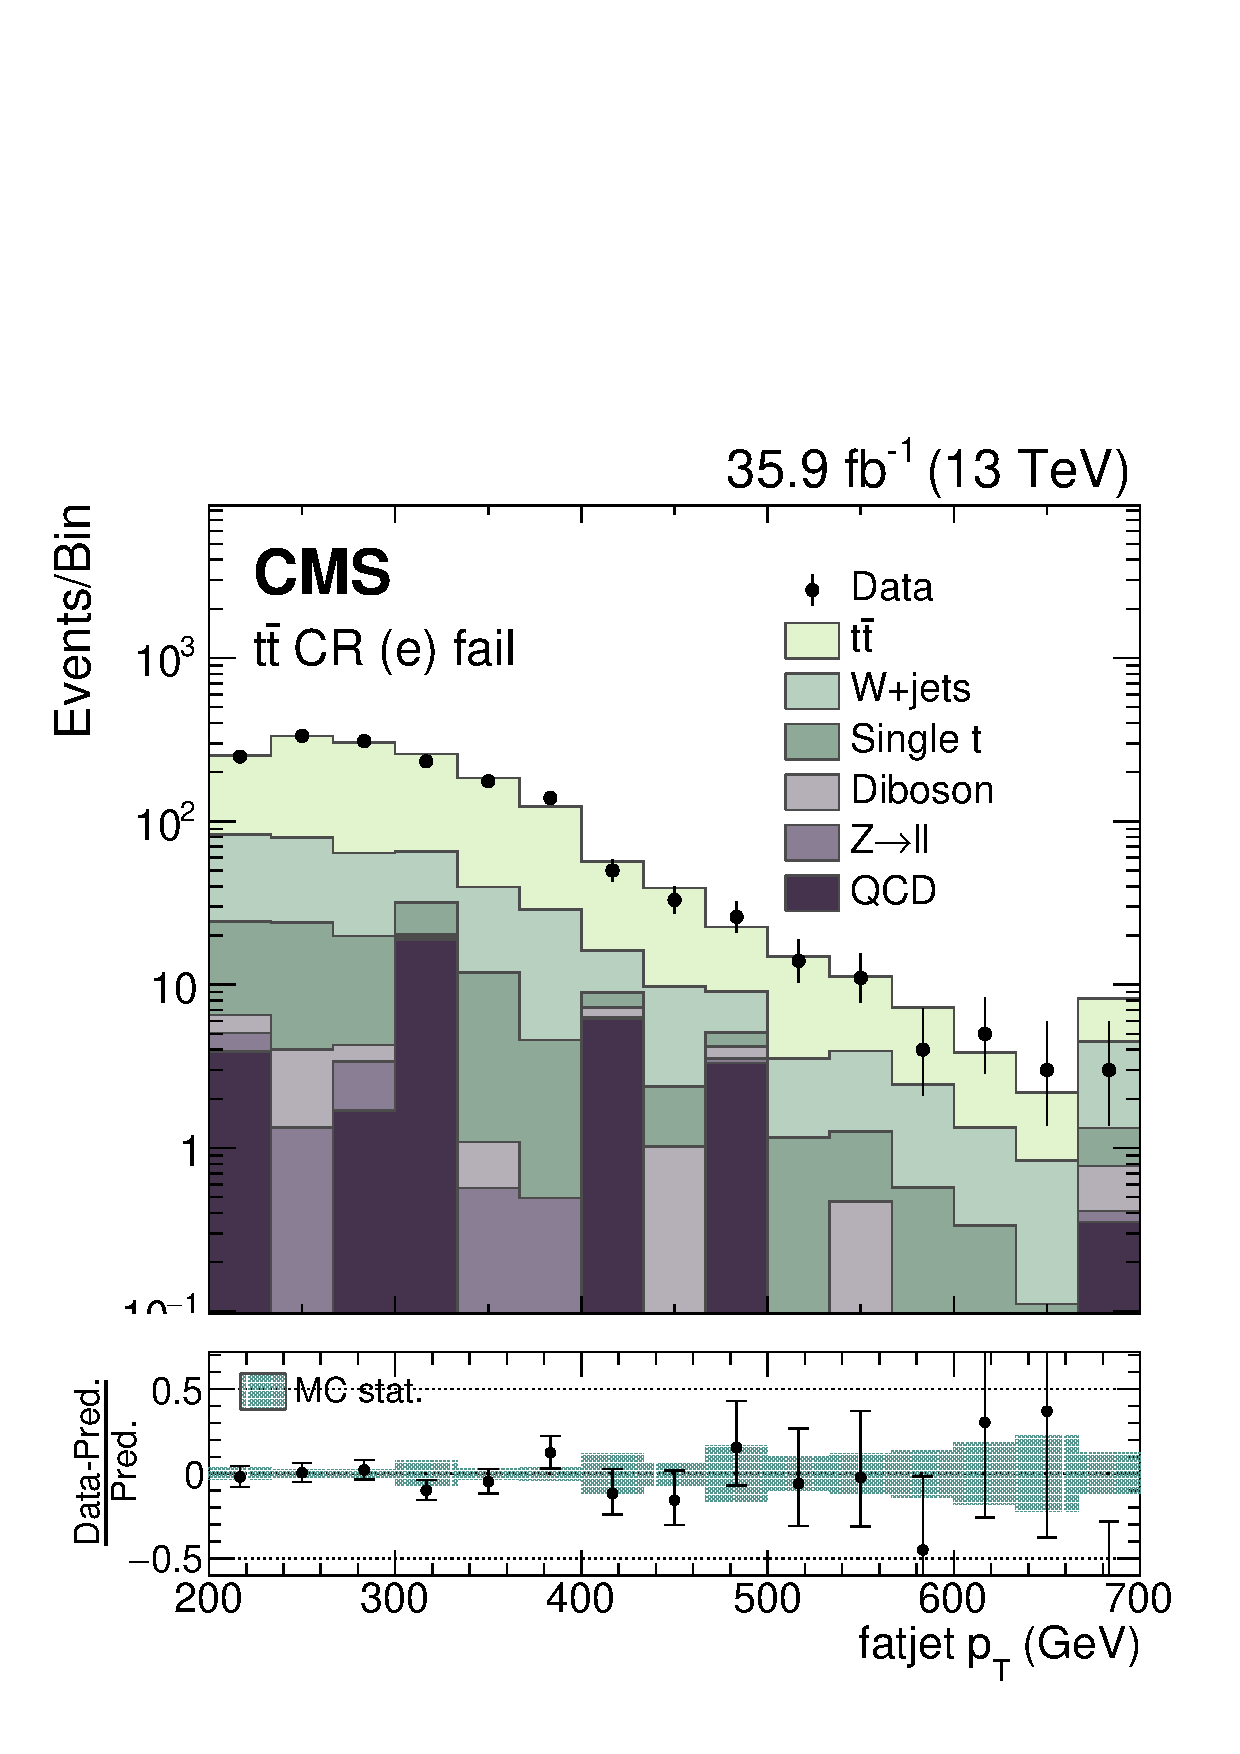
\includegraphics[width=0.4\textwidth]{figures/dataMC/cr_ttbar_el_fail_fj1Pt.pdf}}
 \subfloat{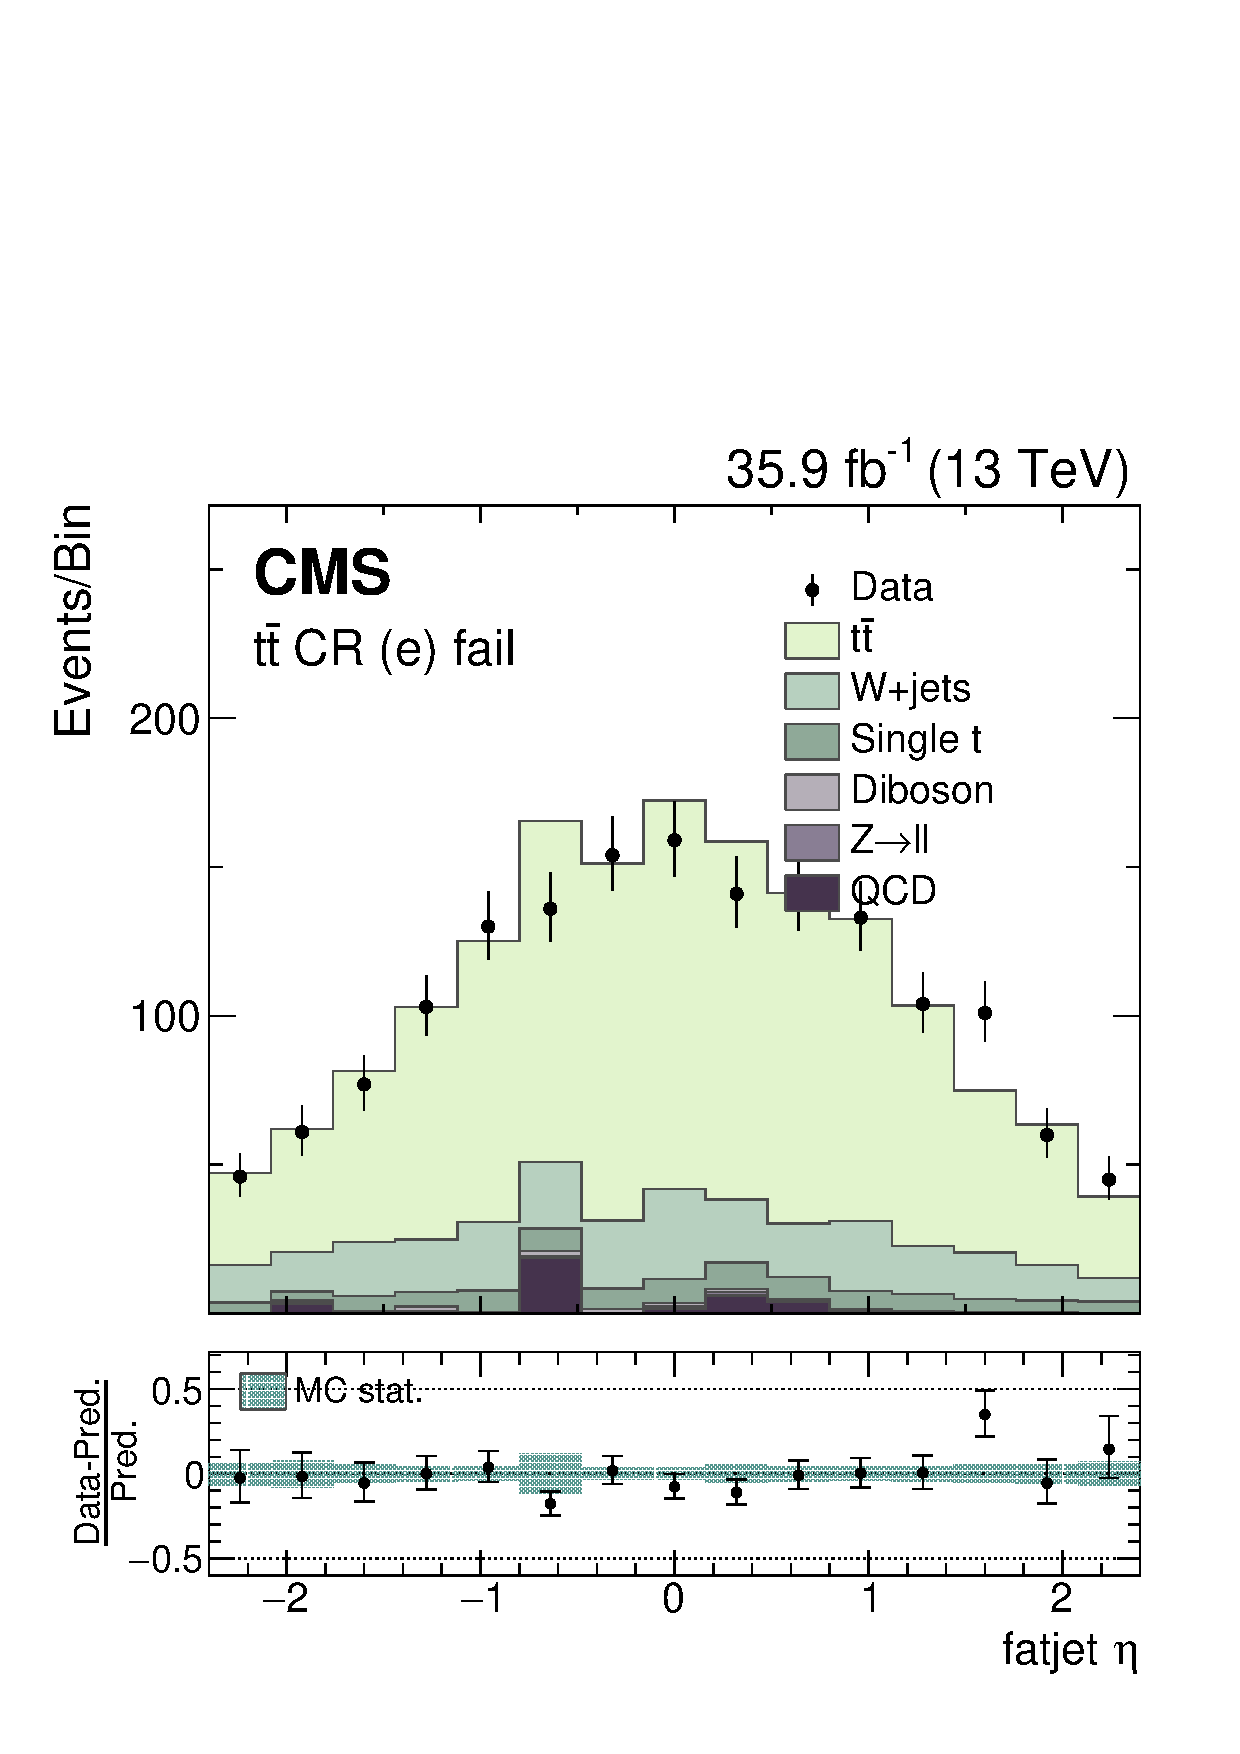
\includegraphics[width=0.4\textwidth]{figures/dataMC/cr_ttbar_el_fail_fj1Eta.pdf}} \\
 \subfloat{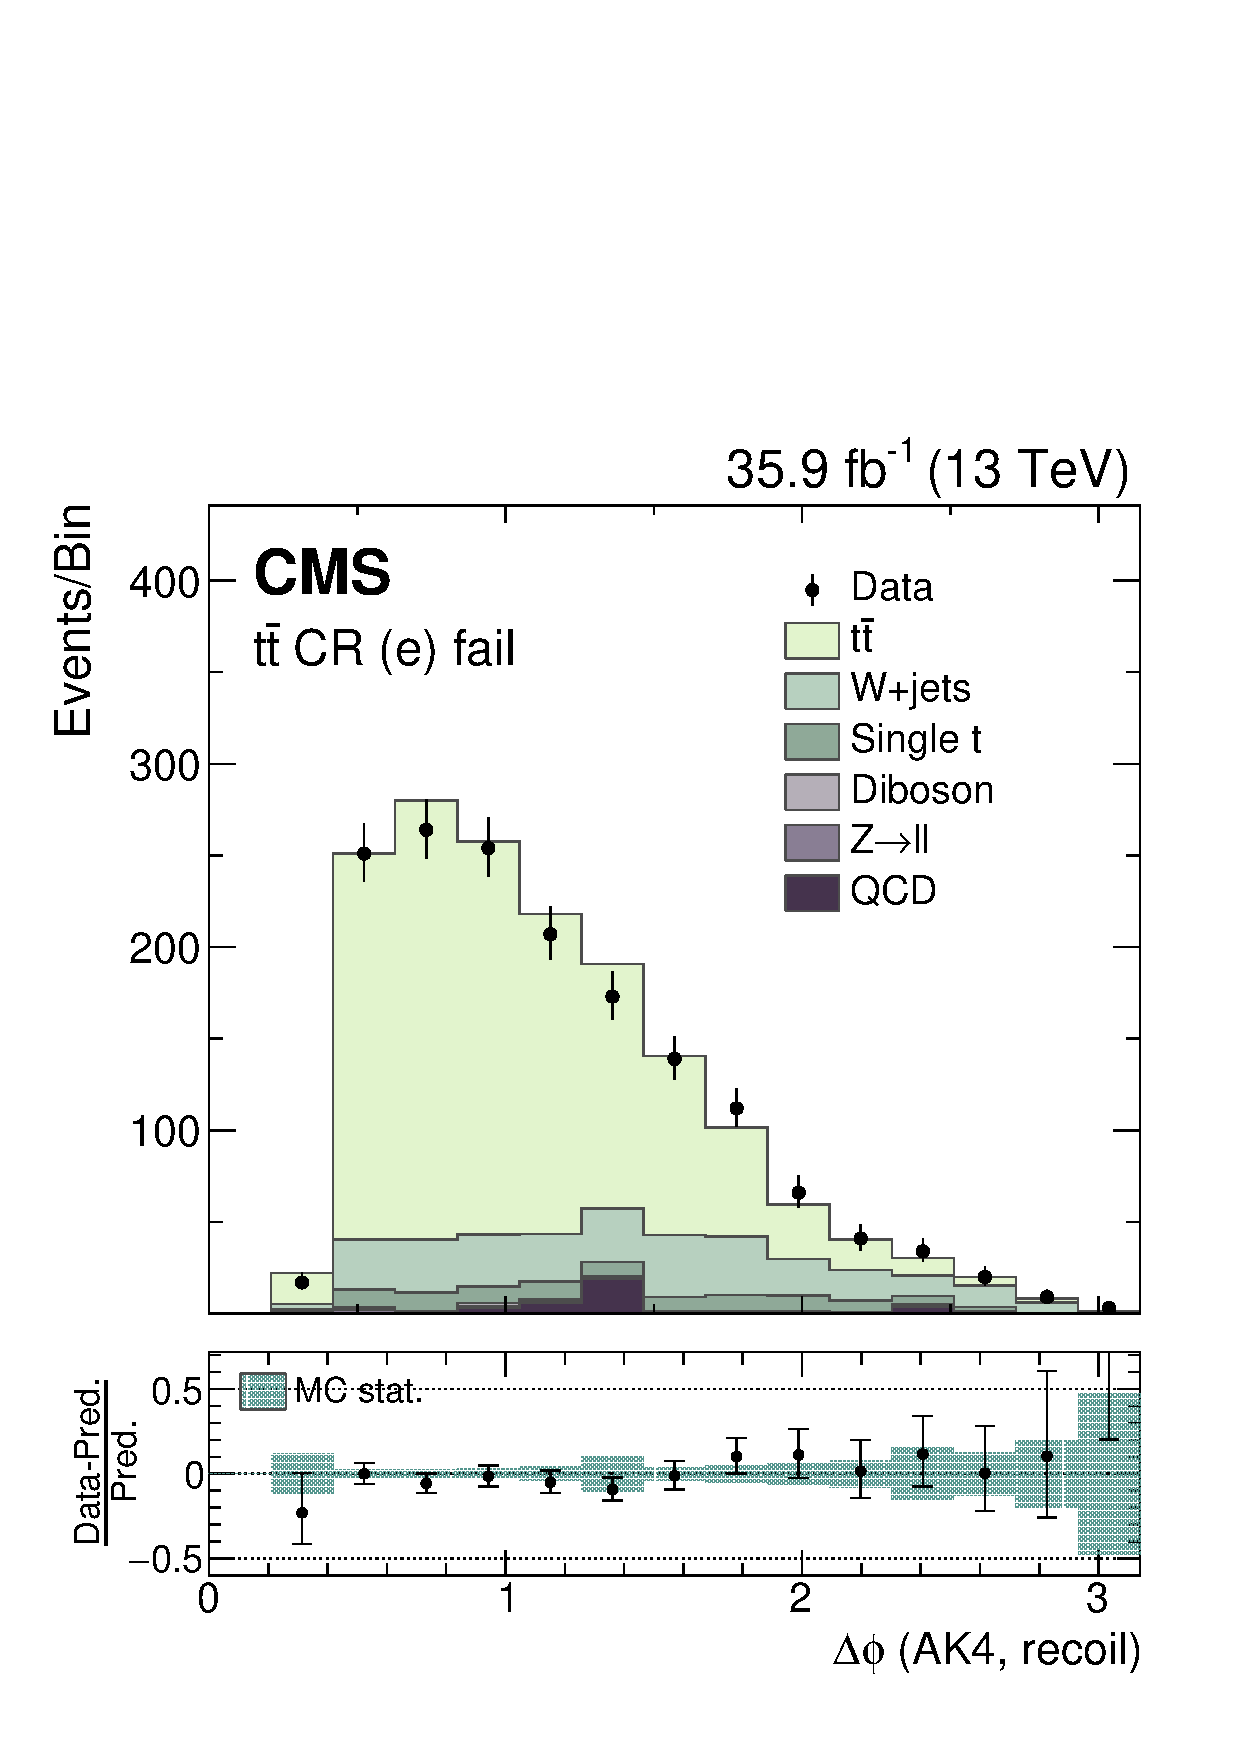
\includegraphics[width=0.4\textwidth]{figures/dataMC/cr_ttbar_el_fail_dphiUW.pdf}} 
 \subfloat{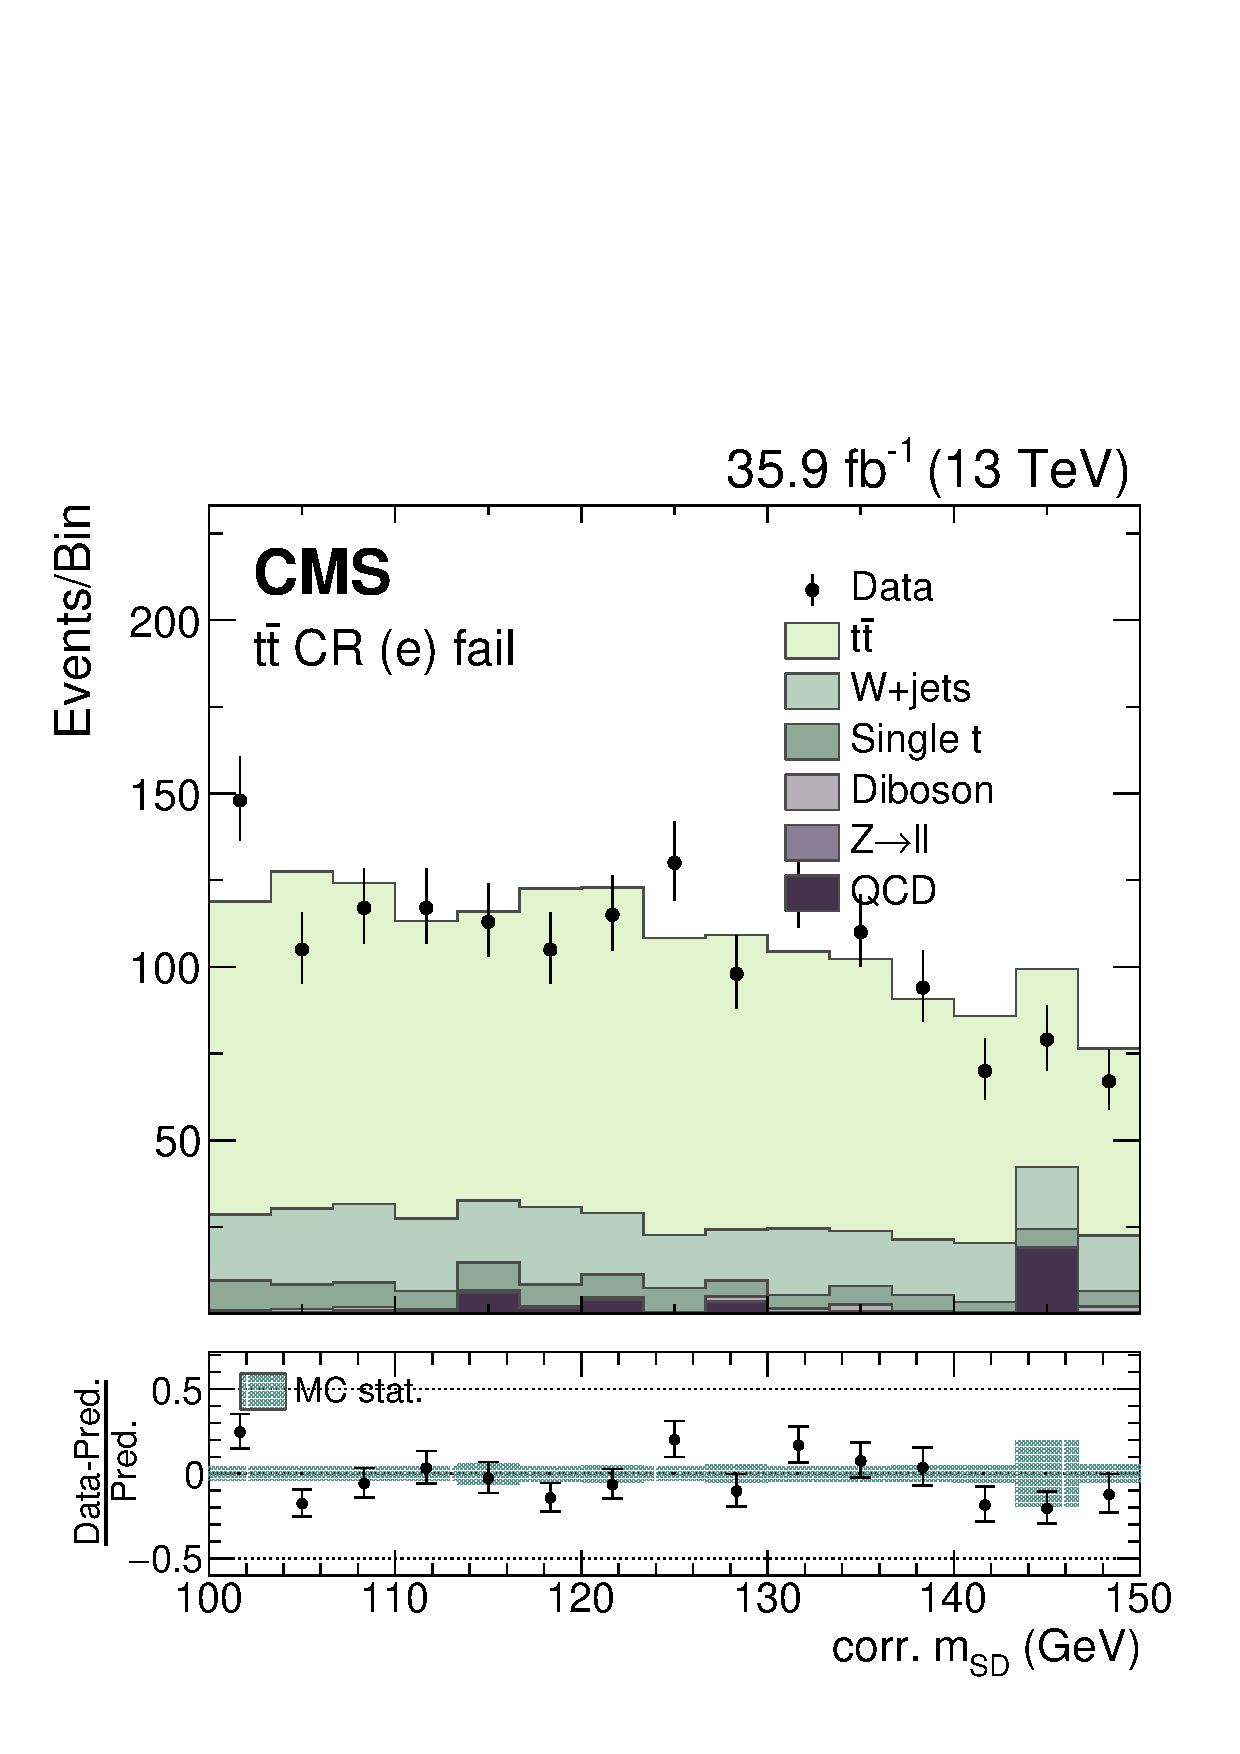
\includegraphics[width=0.4\textwidth]{figures/dataMC/cr_ttbar_el_fail_fj1MSD_corr.pdf}} \\
\caption{Prefit validation plots in the \ttbar fail CR (electron channel).}
\label{Fig_cr_ttbar_el_1}
\end{figure}


\clearpage


\begin{figure}
\centering
 \subfloat{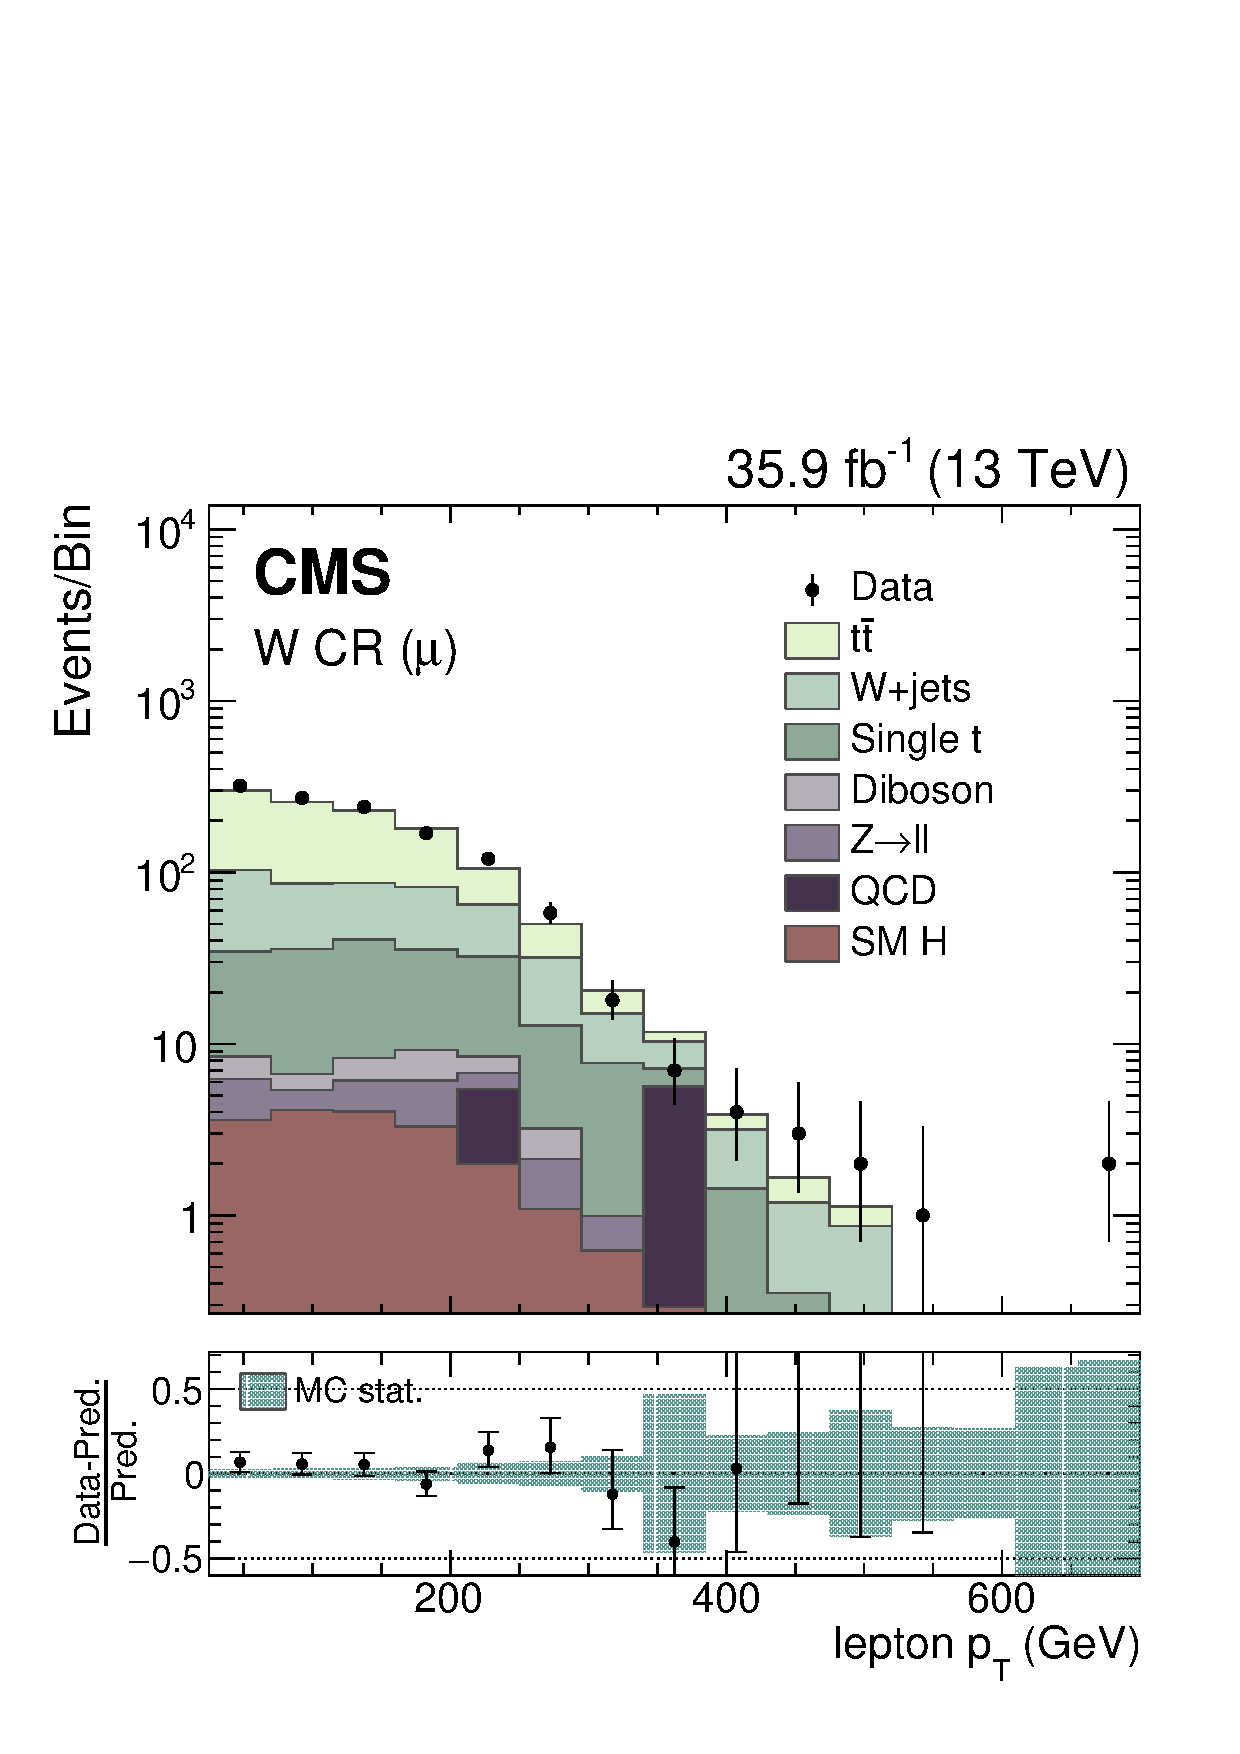
\includegraphics[width=0.4\textwidth]{figures/dataMC/cr_w_mu_lep1Pt.pdf}}
 \subfloat{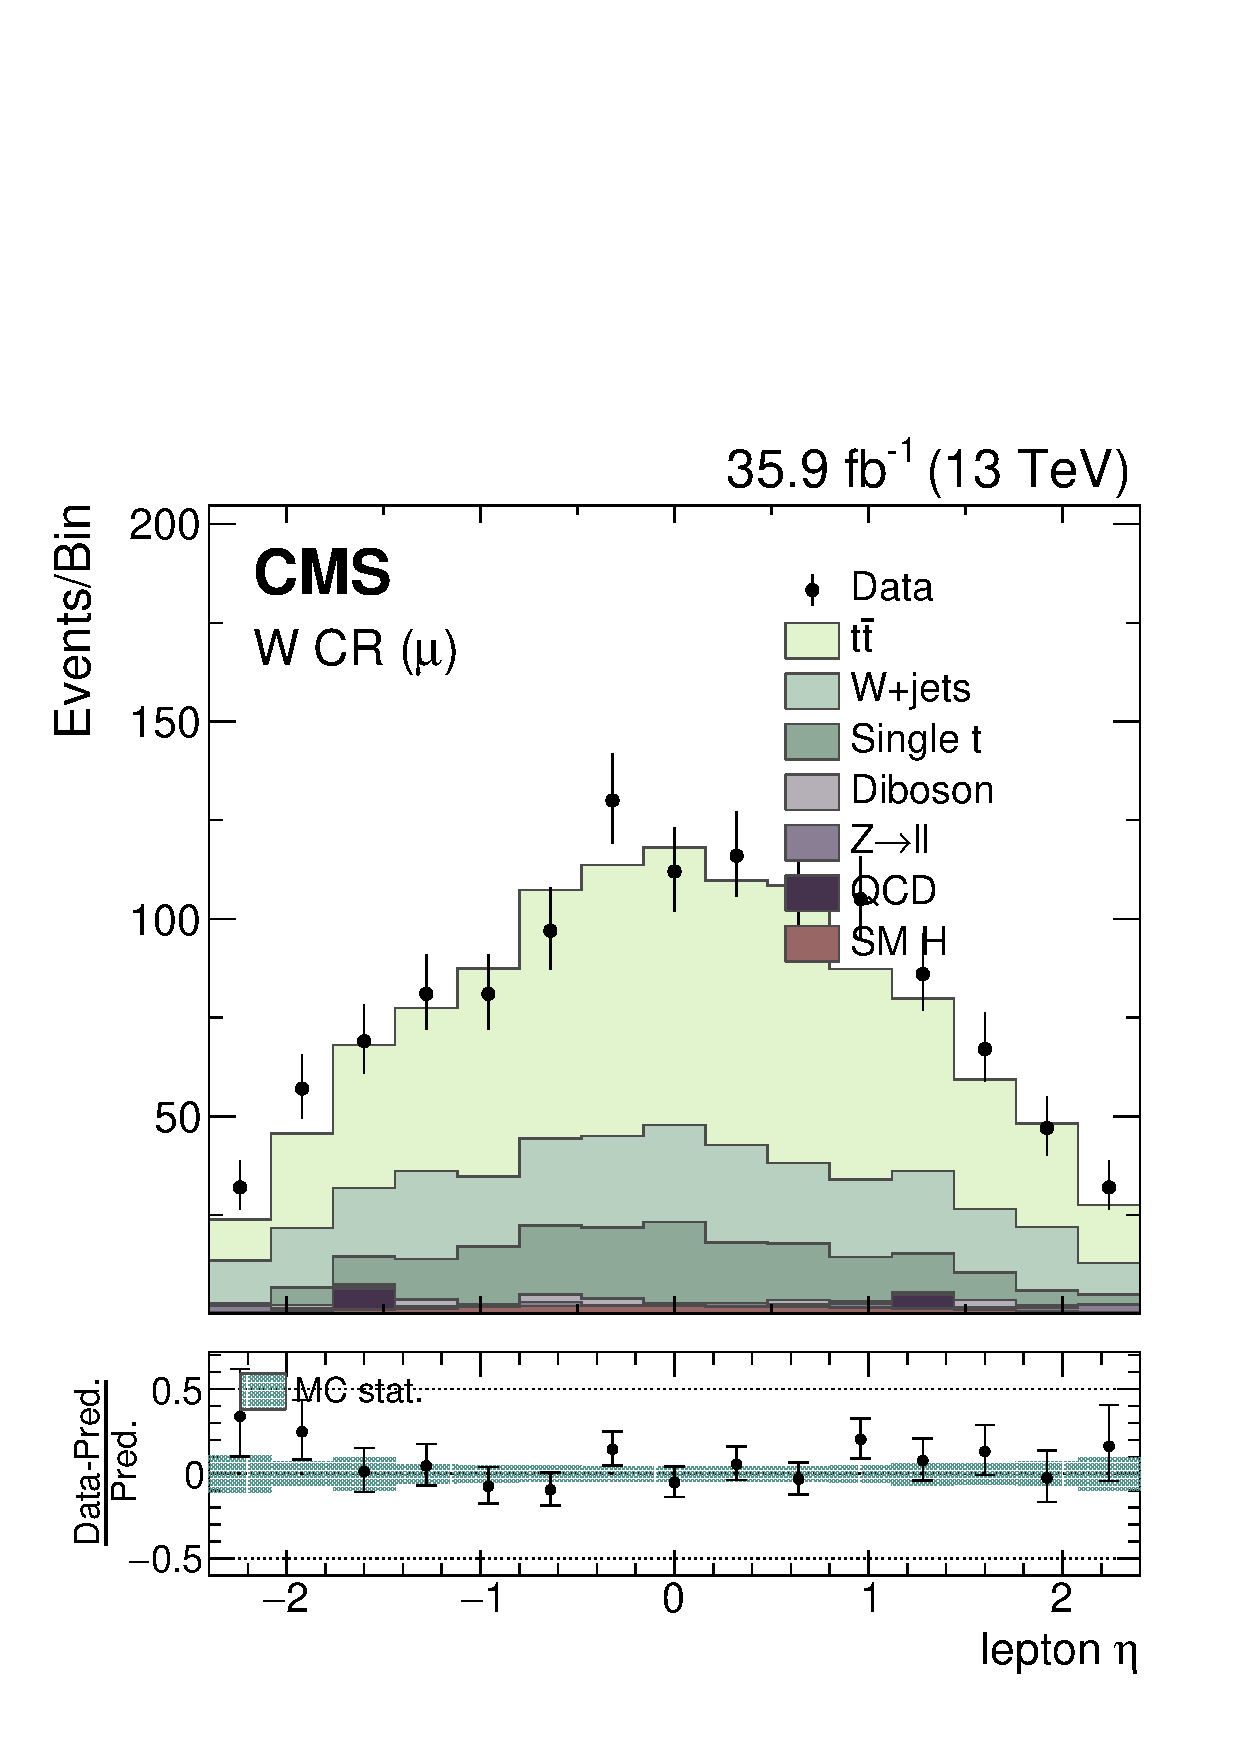
\includegraphics[width=0.4\textwidth]{figures/dataMC/cr_w_mu_lep1Eta.pdf}} \\
 \subfloat{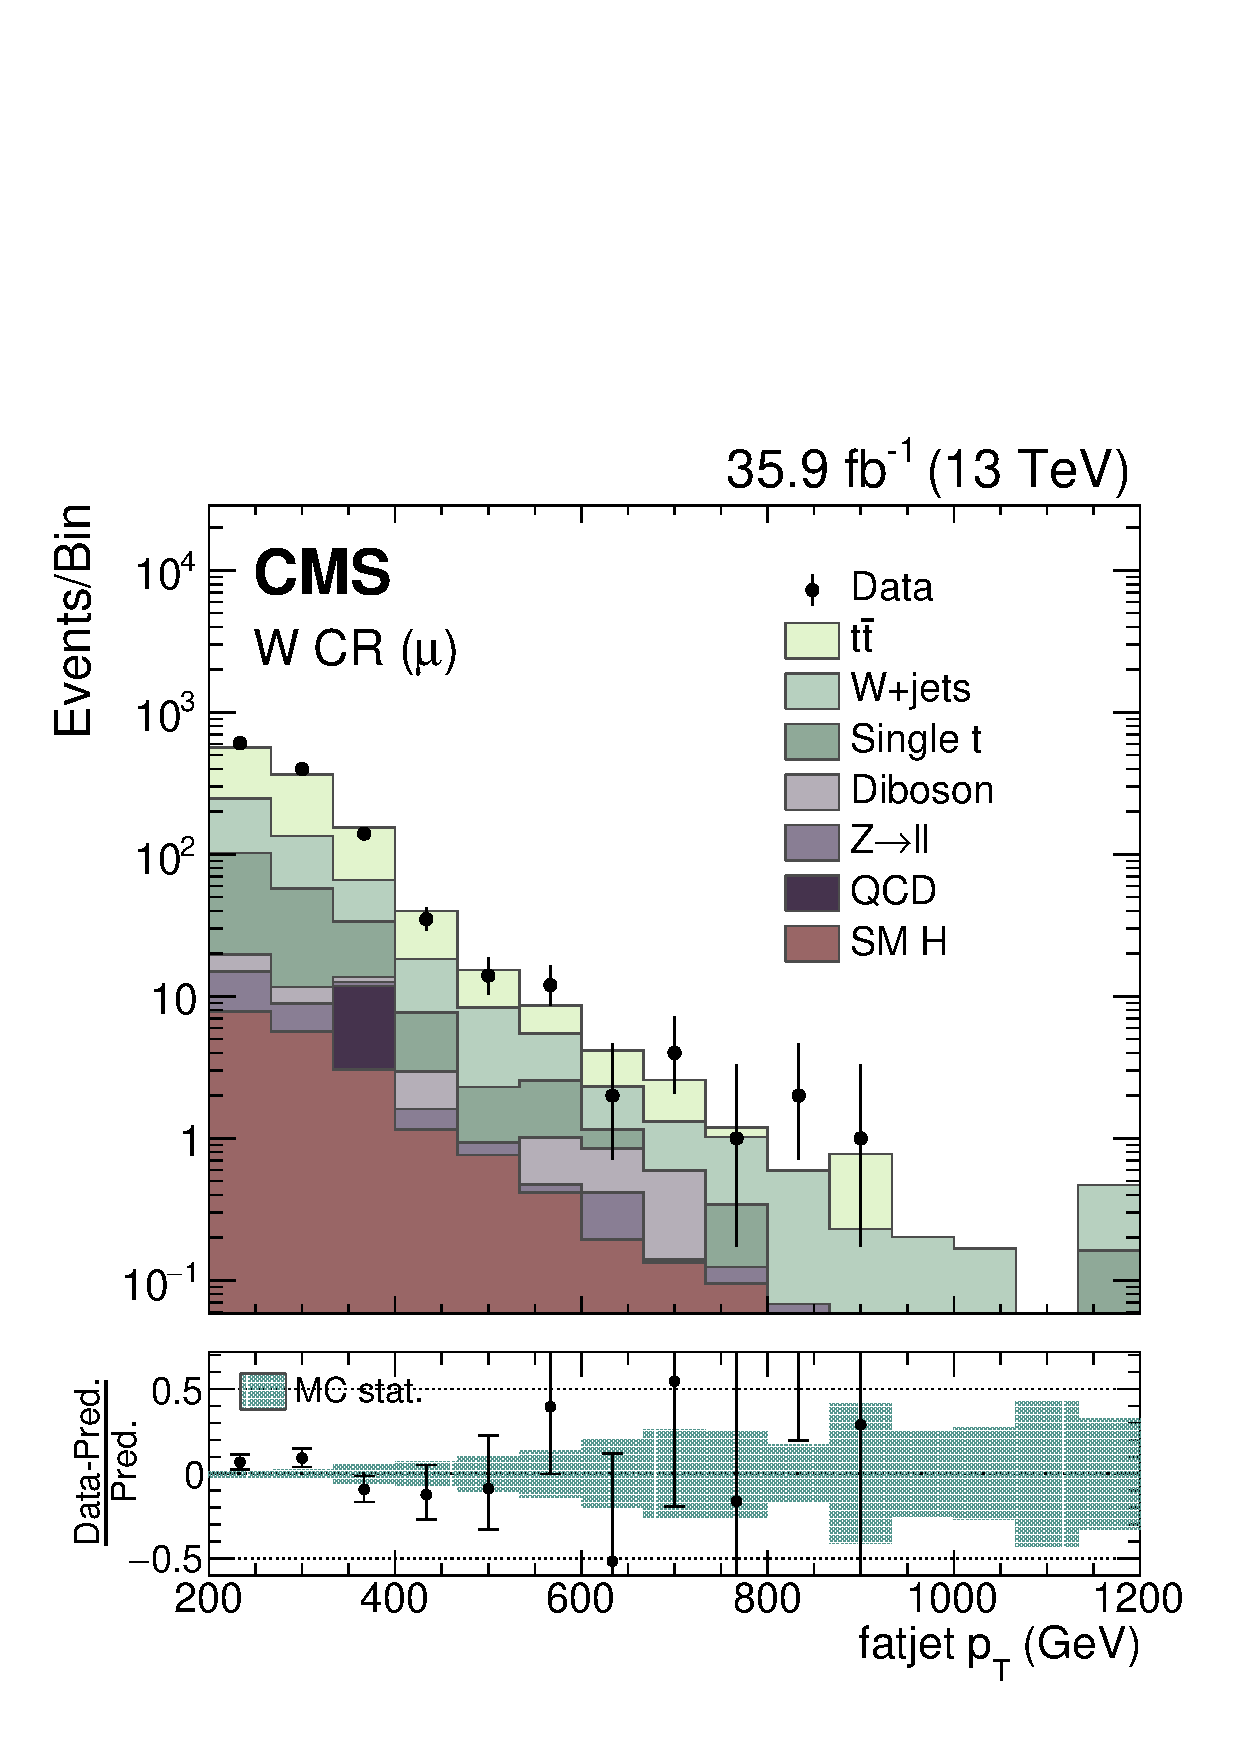
\includegraphics[width=0.4\textwidth]{figures/dataMC/cr_w_mu_fj1Pt.pdf}}
 \subfloat{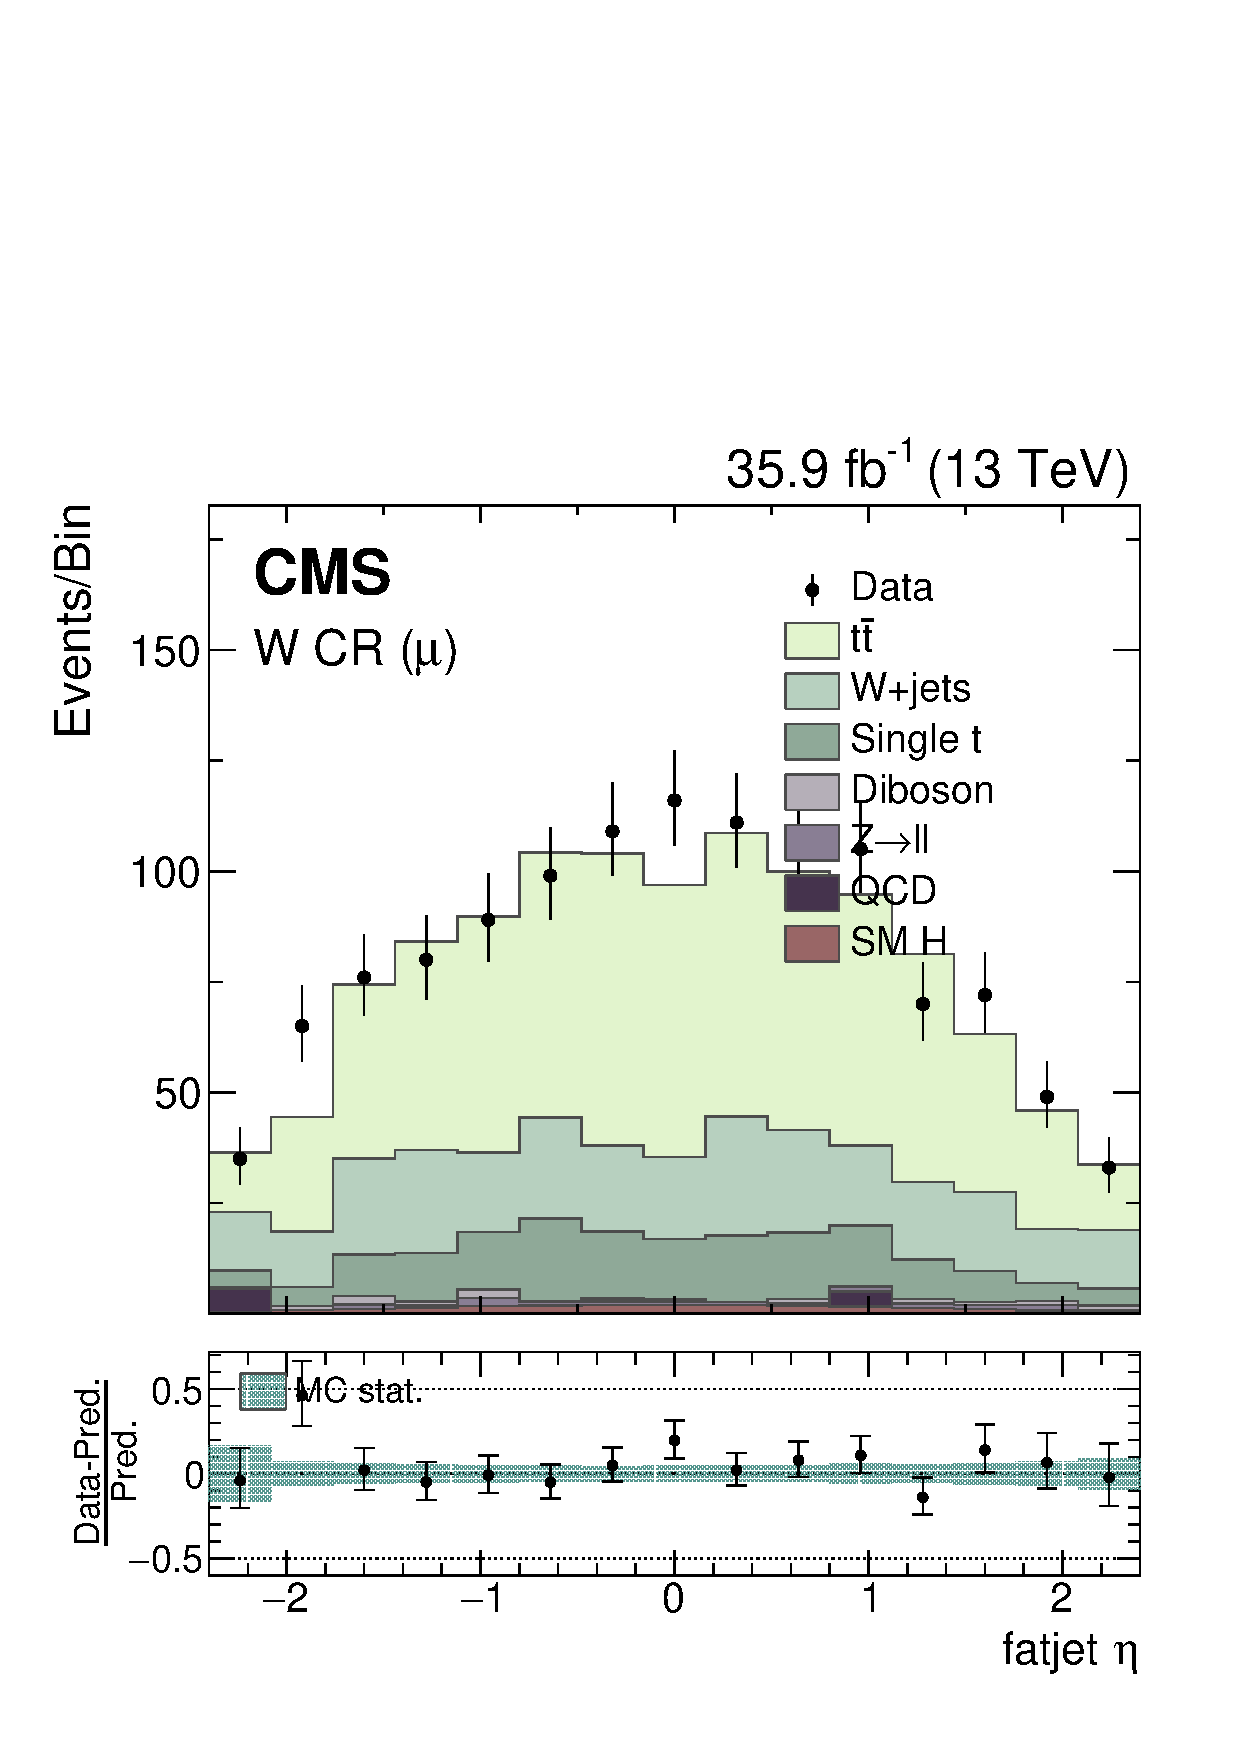
\includegraphics[width=0.4\textwidth]{figures/dataMC/cr_w_mu_fj1Eta.pdf}} \\
 \subfloat{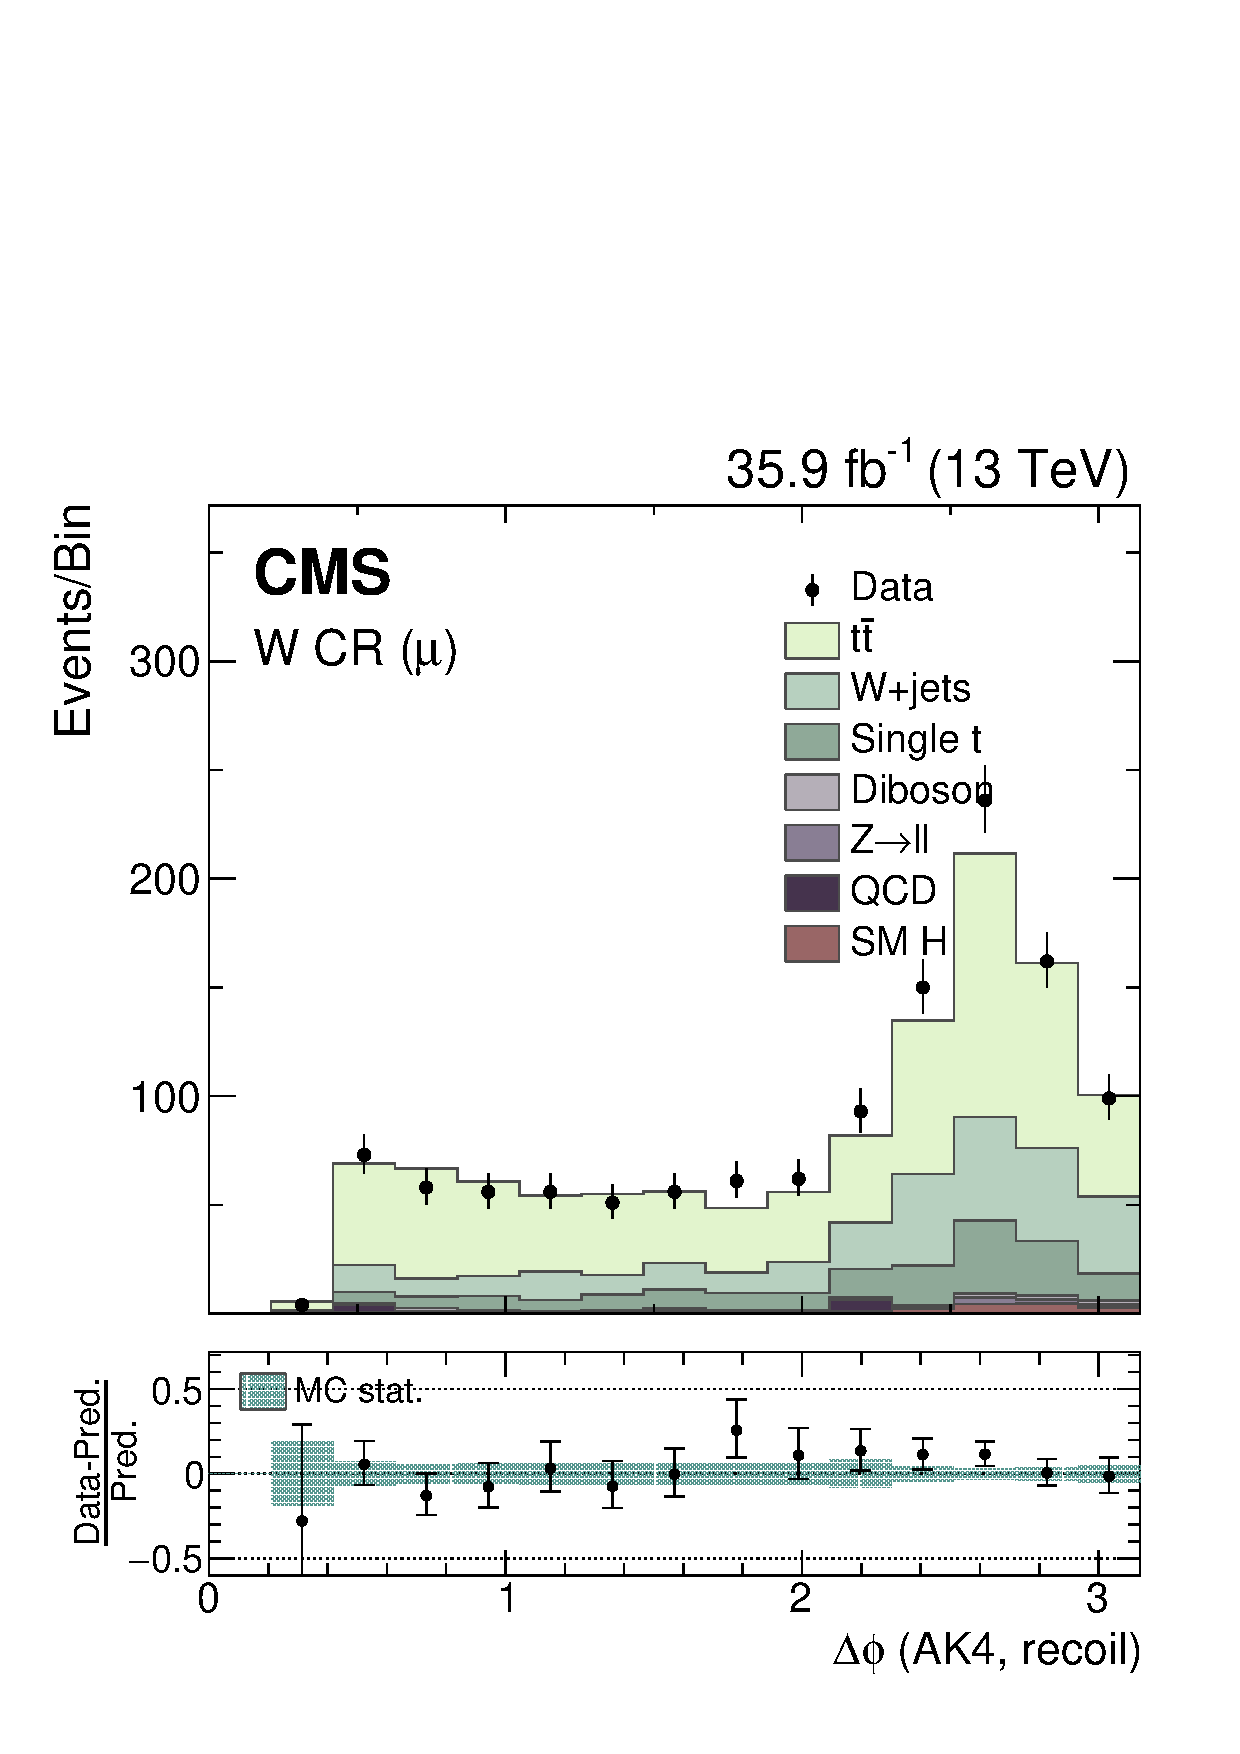
\includegraphics[width=0.4\textwidth]{figures/dataMC/cr_w_mu_dphiUW.pdf}} 
 \subfloat{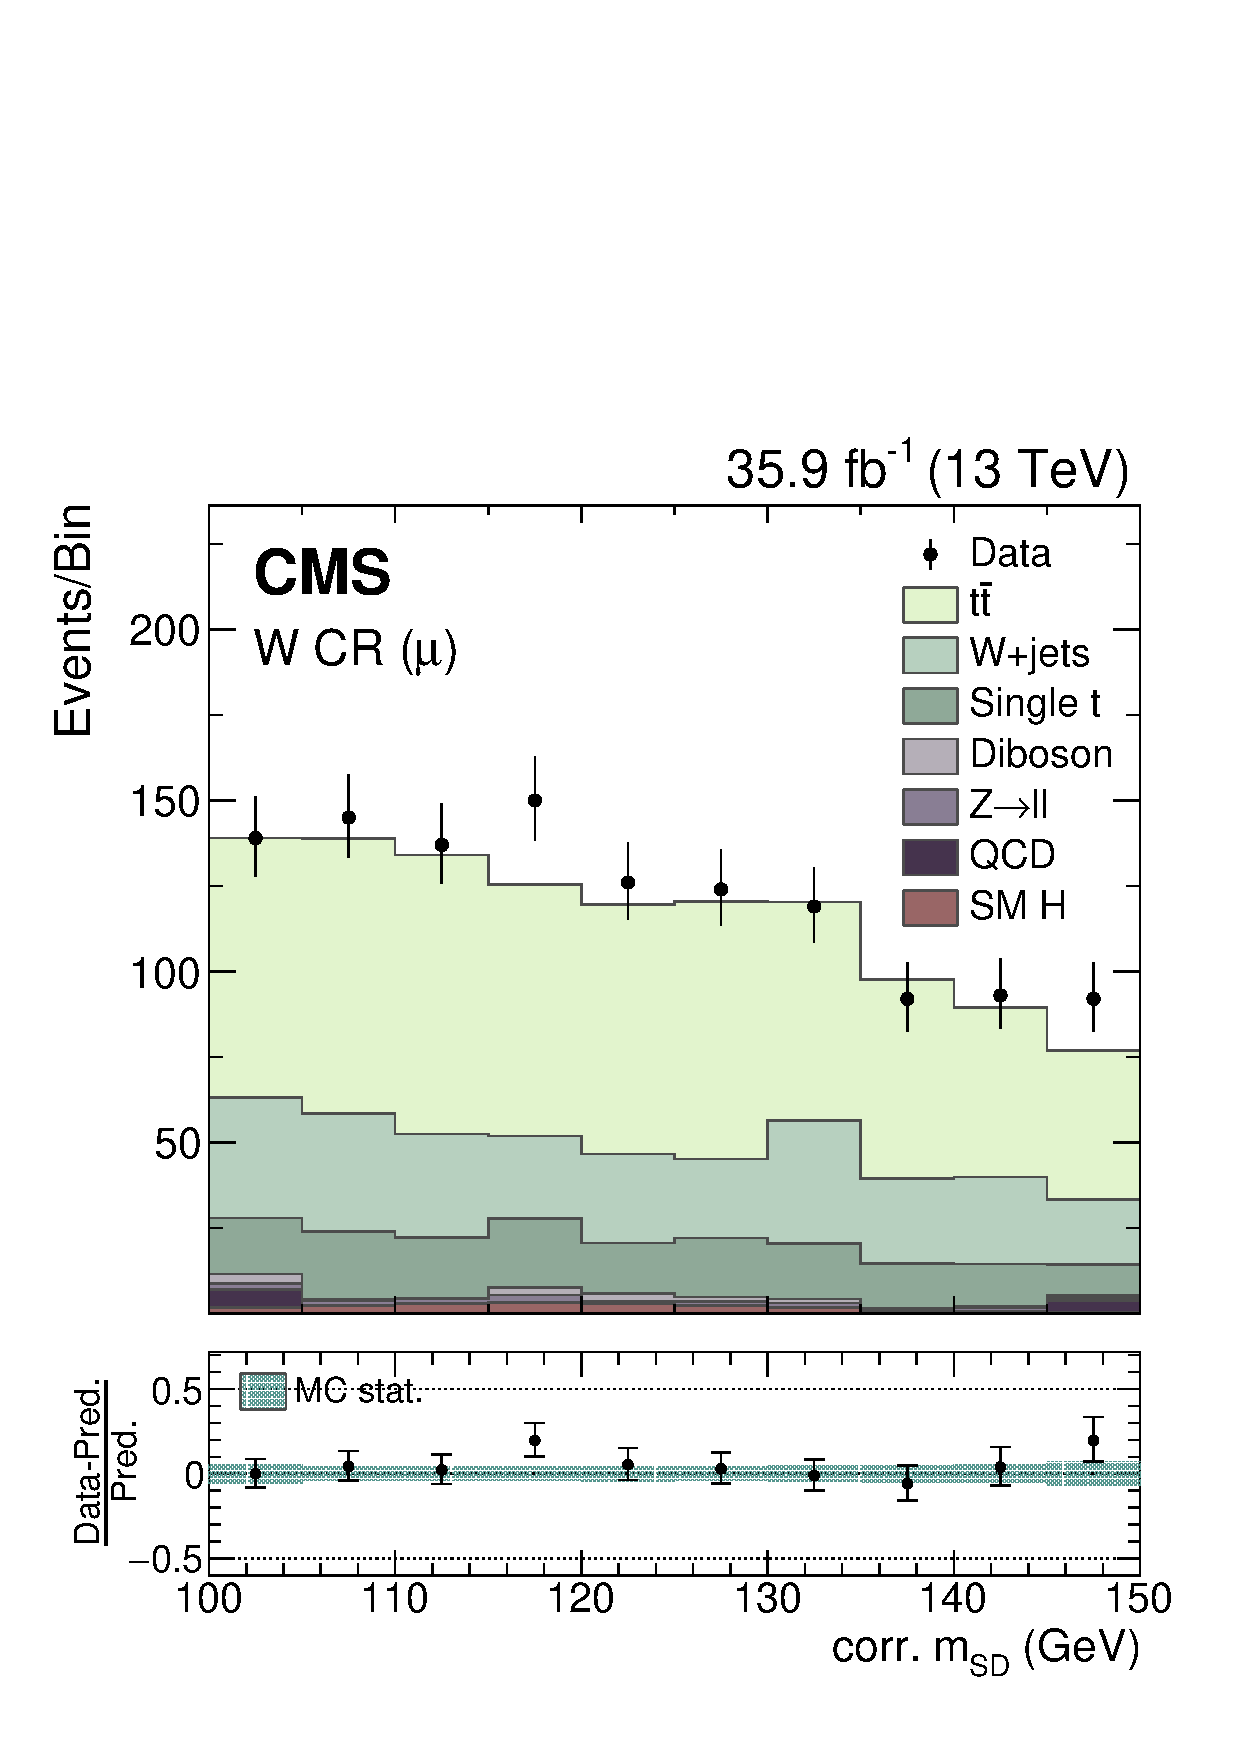
\includegraphics[width=0.4\textwidth]{figures/dataMC/cr_w_mu_fj1MSD_corr.pdf}} \\
\caption{Prefit validation plots in the W CR (muon channel).}
\label{Fig_cr_w_mu_1}
\end{figure}

\clearpage


\begin{figure}
\centering
 \subfloat{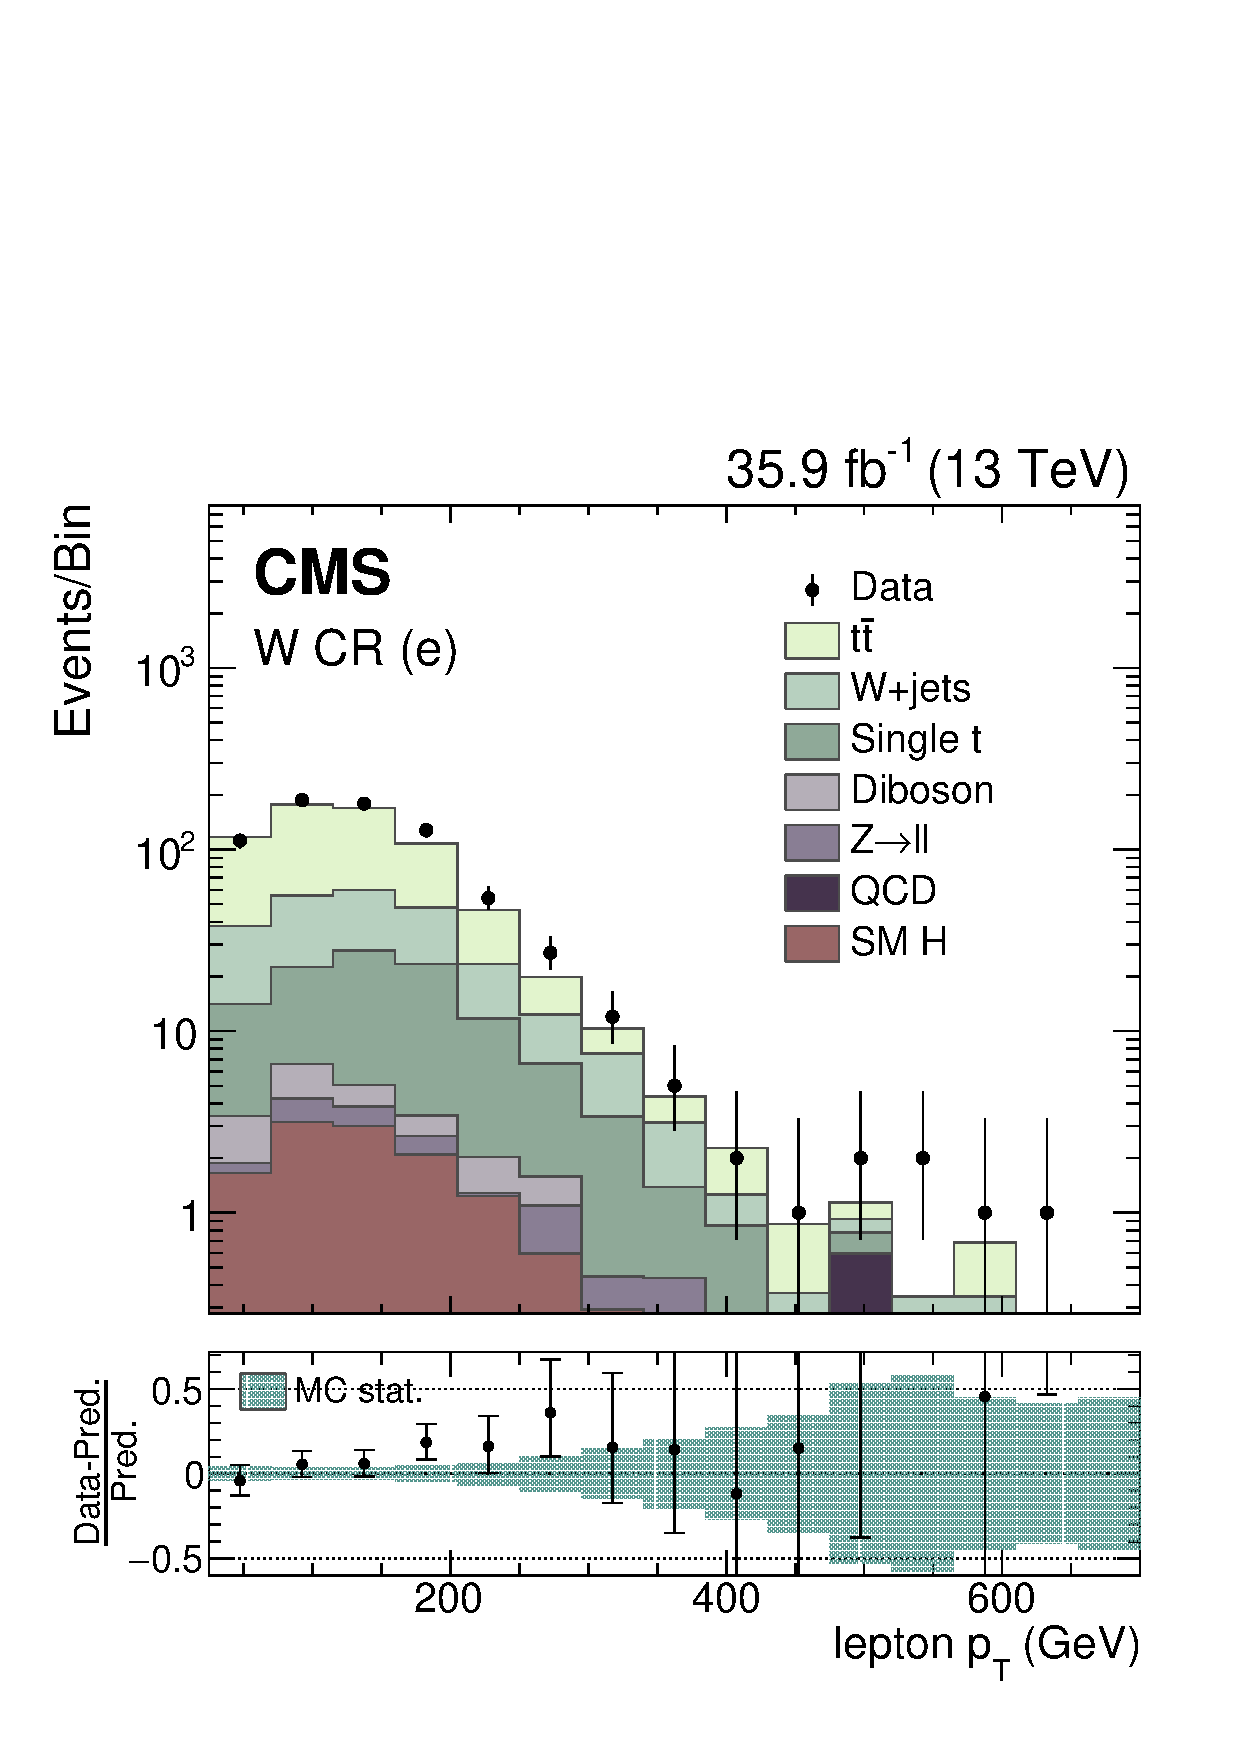
\includegraphics[width=0.4\textwidth]{figures/dataMC/cr_w_el_lep1Pt.pdf}}
 \subfloat{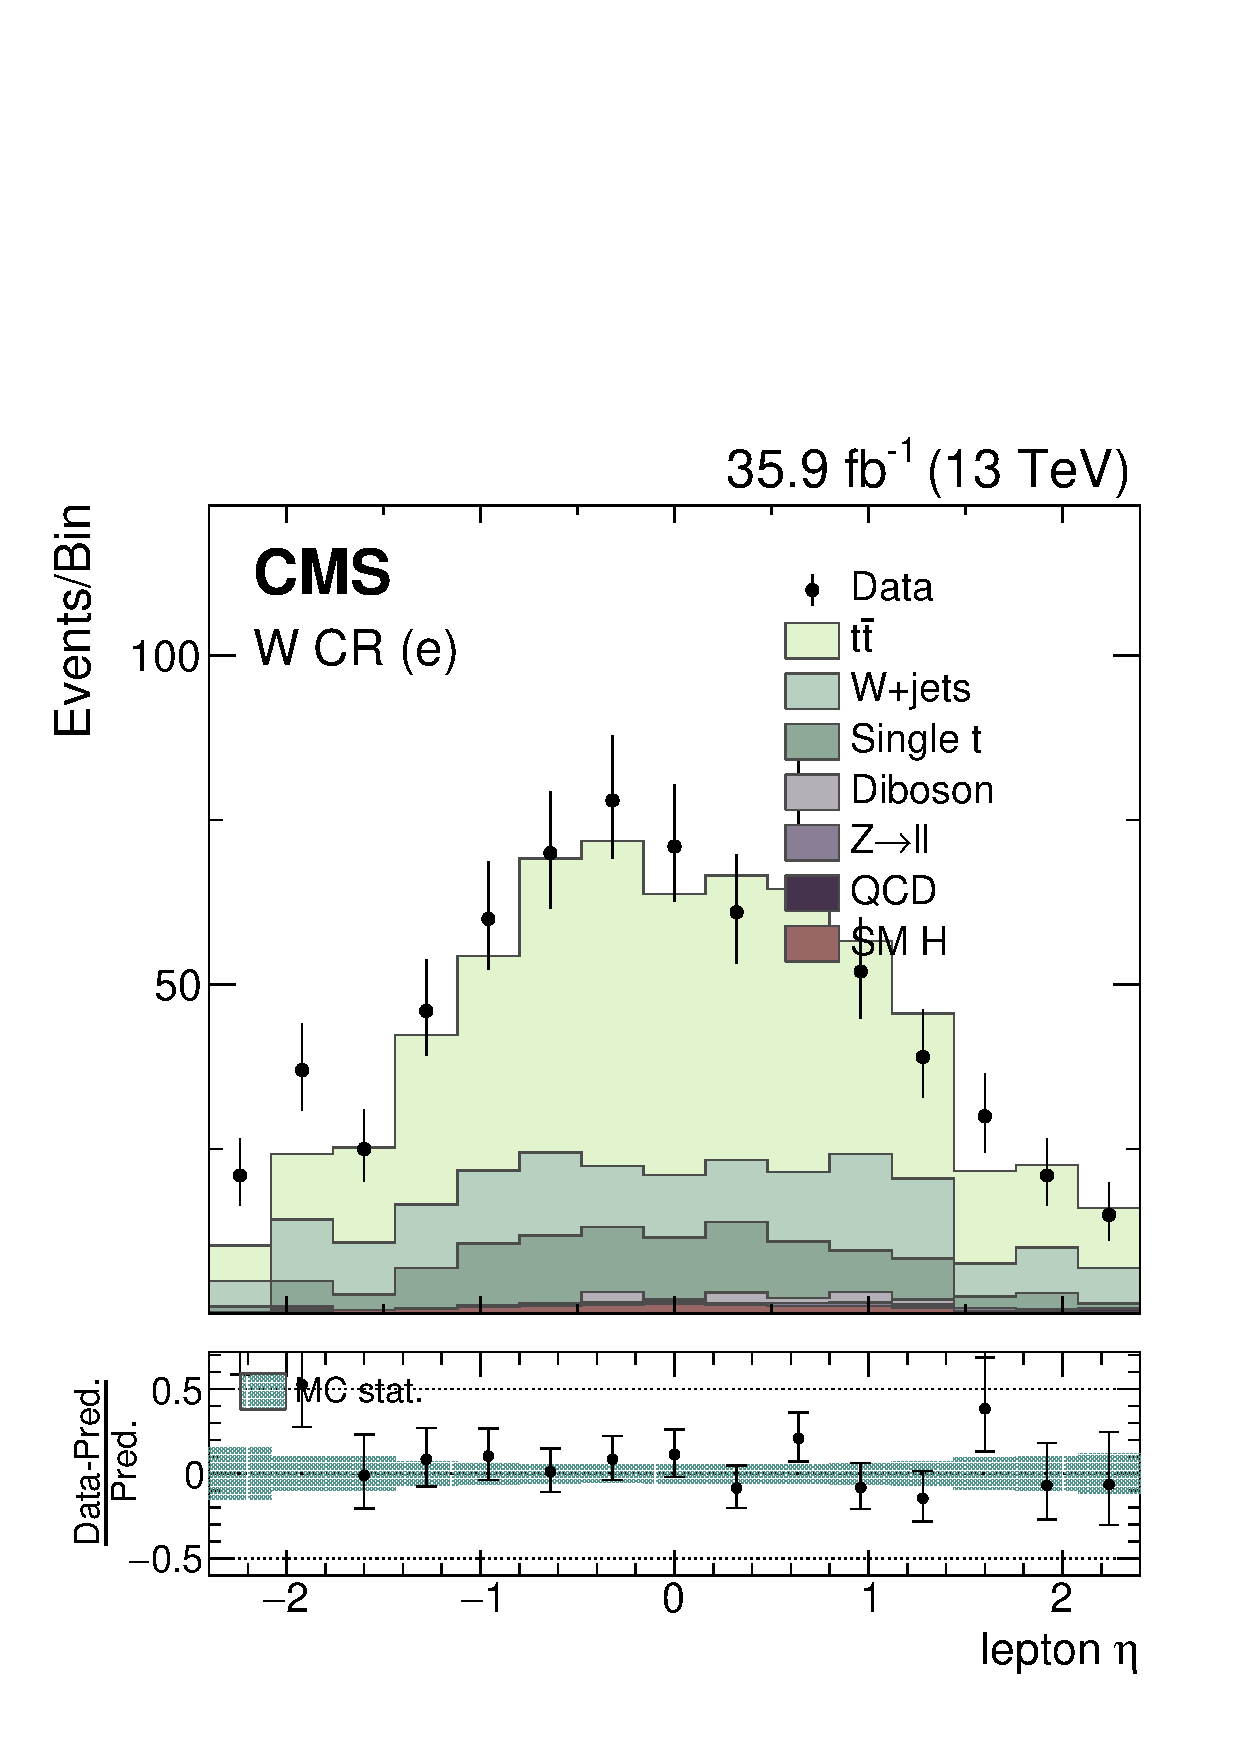
\includegraphics[width=0.4\textwidth]{figures/dataMC/cr_w_el_lep1Eta.pdf}} \\
 \subfloat{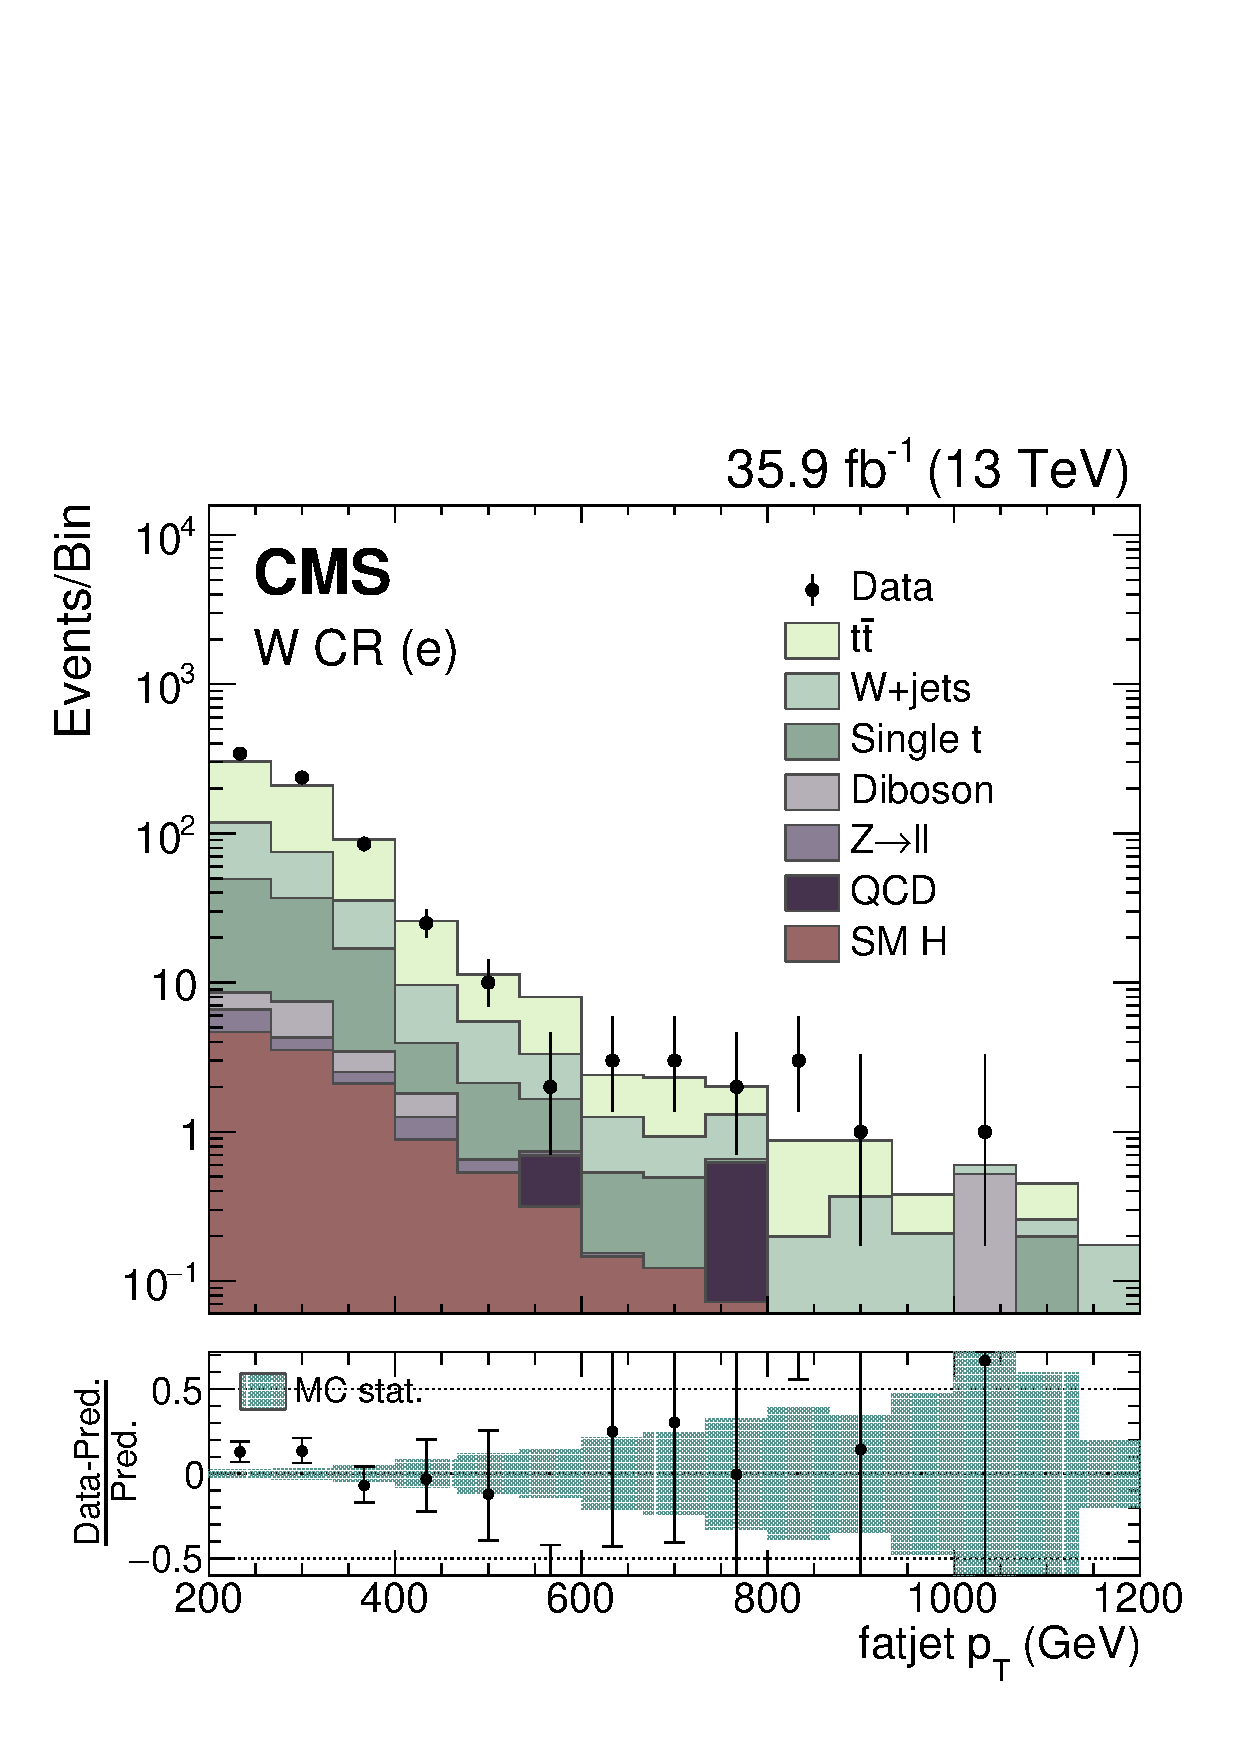
\includegraphics[width=0.4\textwidth]{figures/dataMC/cr_w_el_fj1Pt.pdf}}
 \subfloat{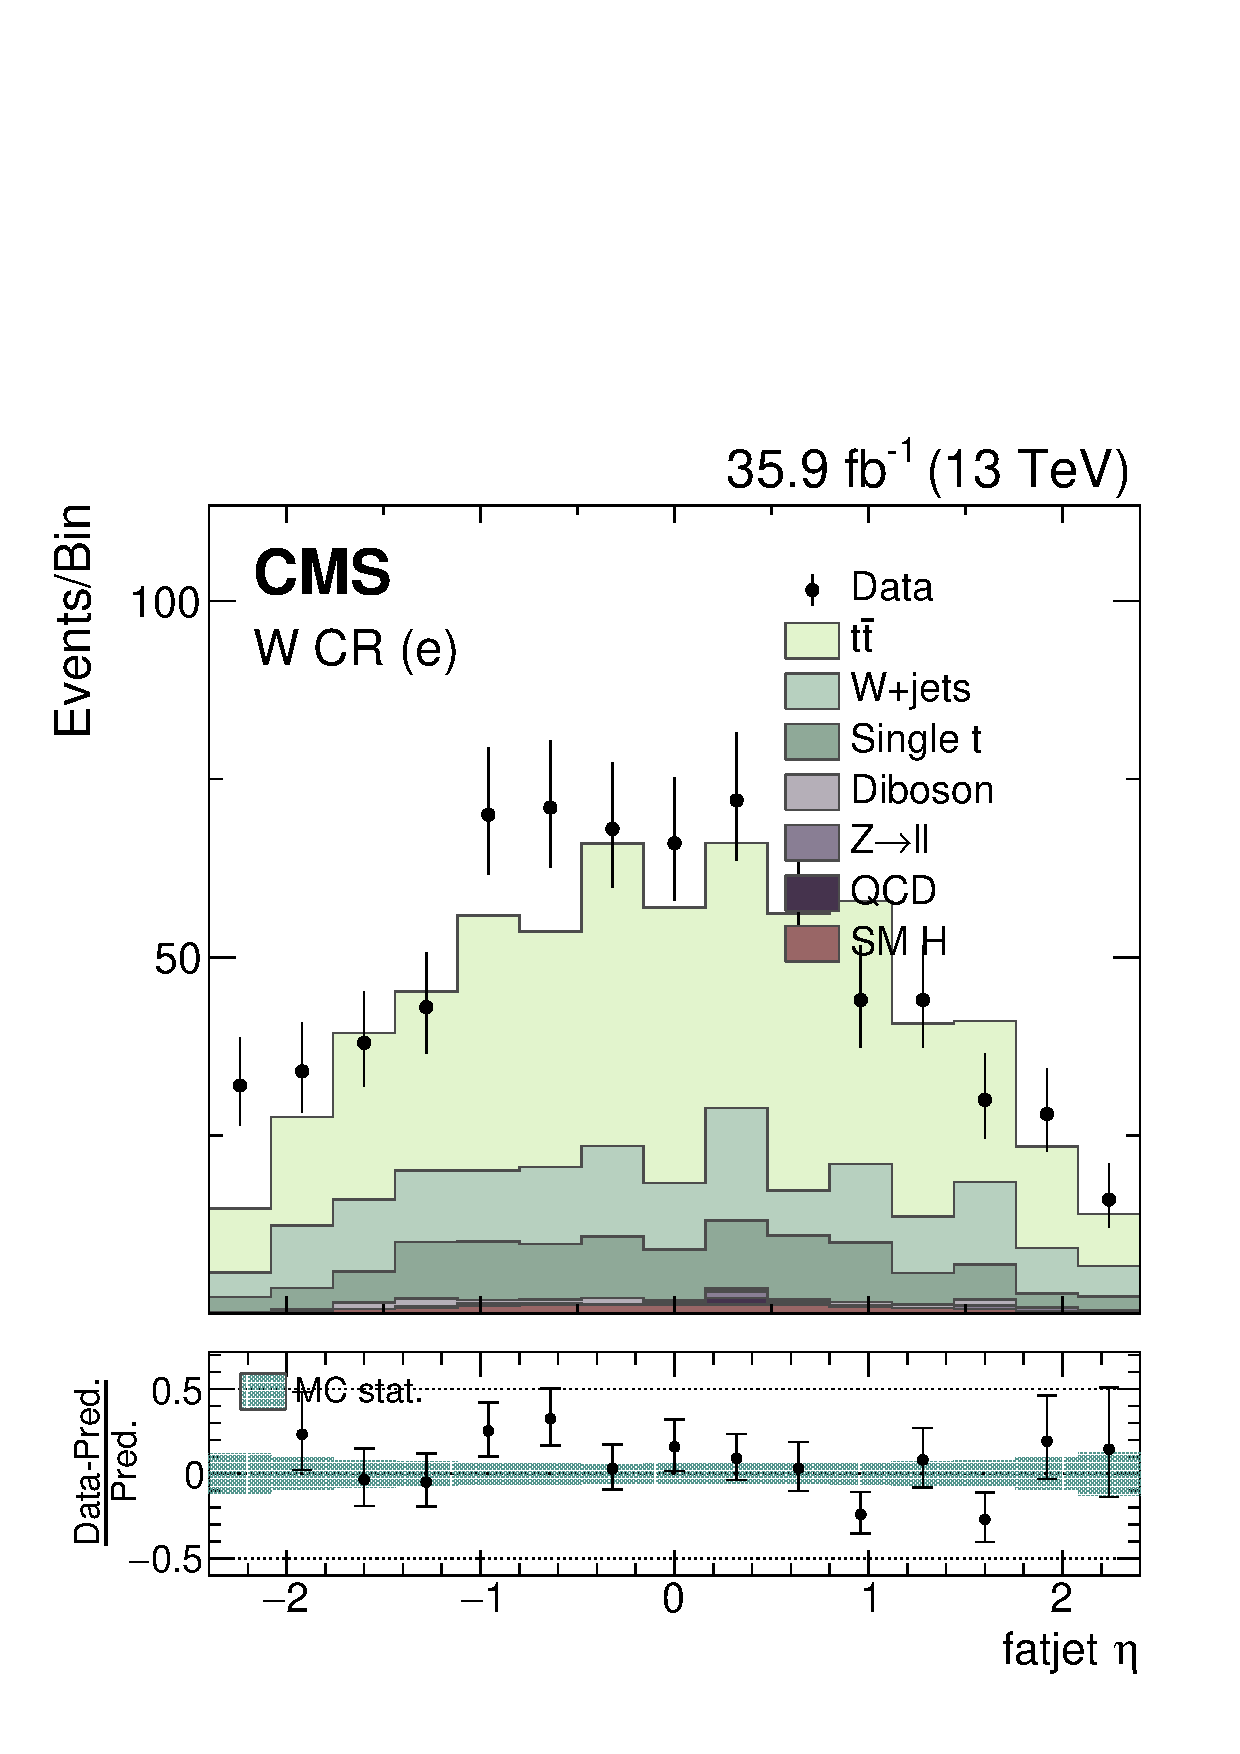
\includegraphics[width=0.4\textwidth]{figures/dataMC/cr_w_el_fj1Eta.pdf}} \\
 \subfloat{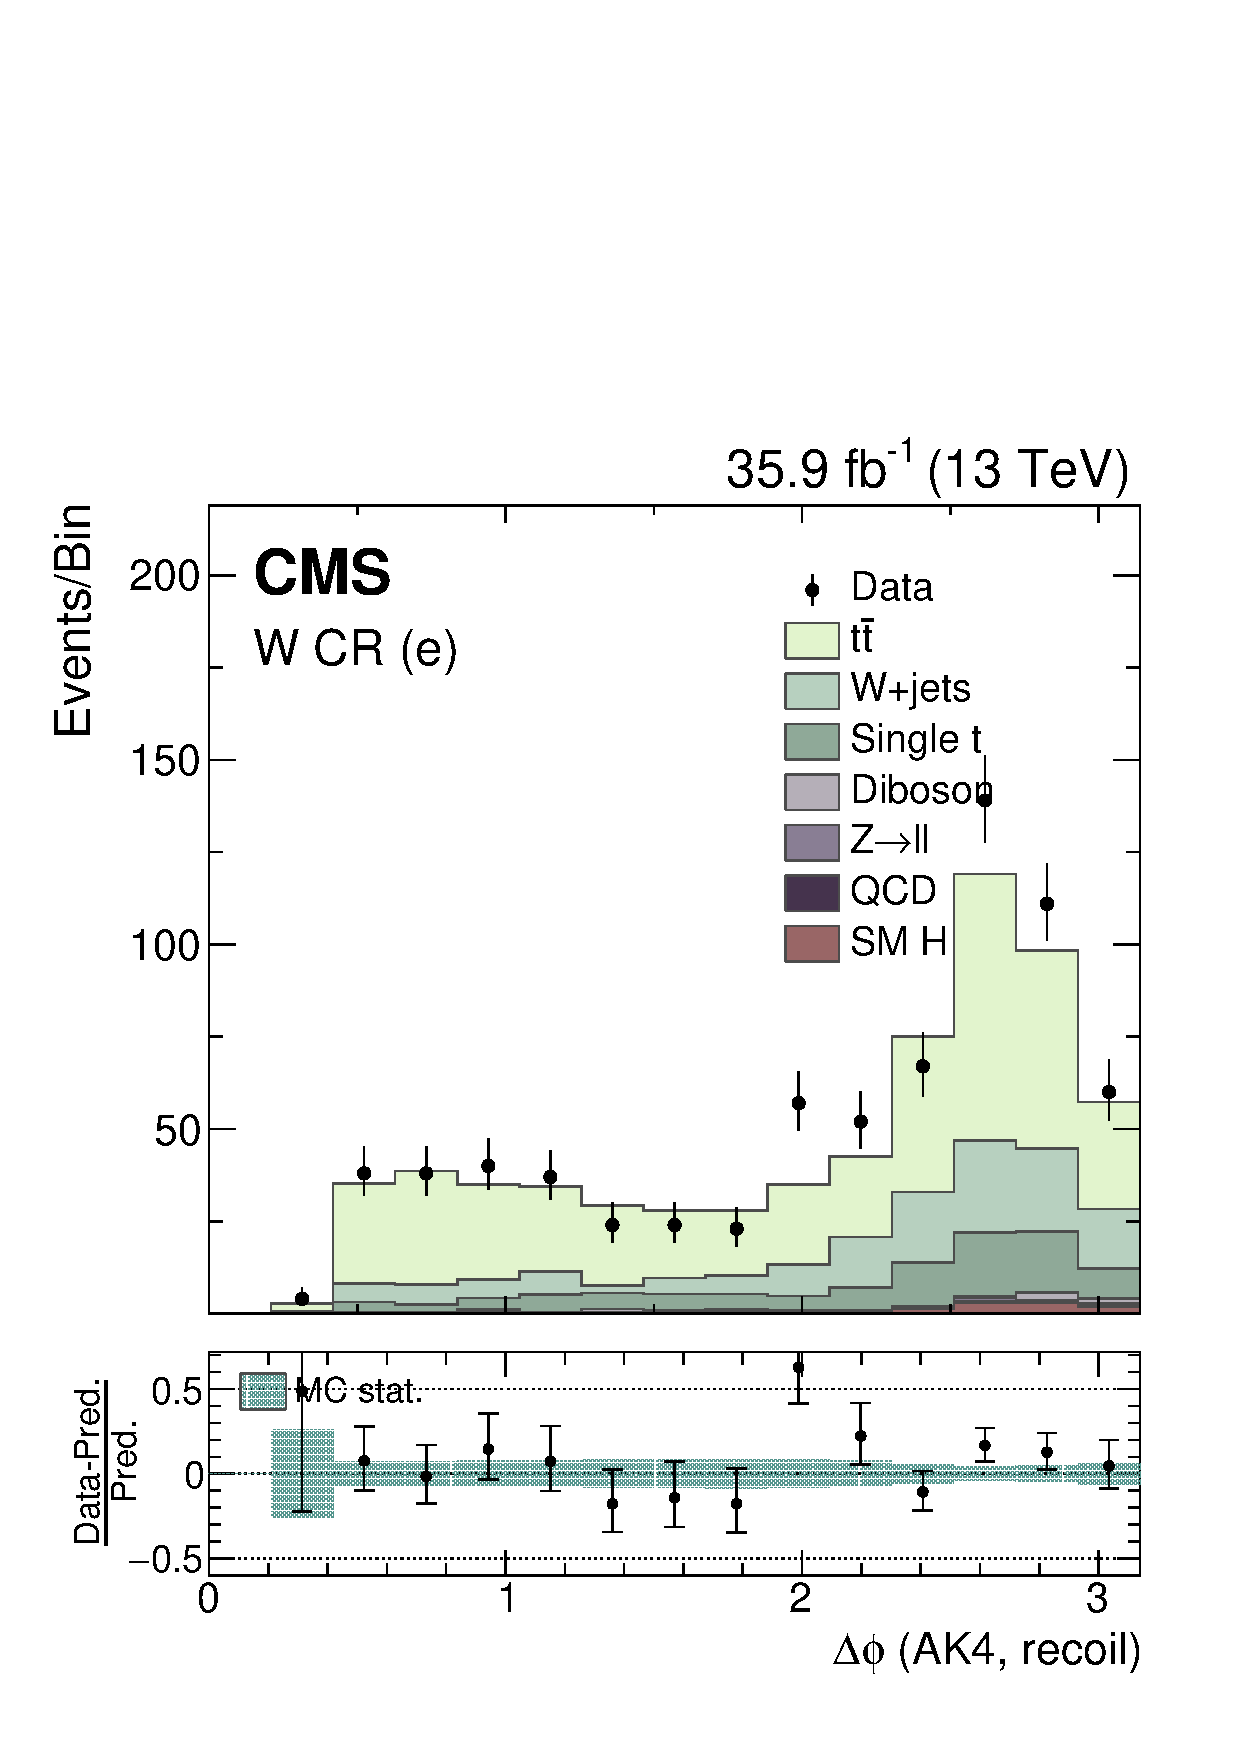
\includegraphics[width=0.4\textwidth]{figures/dataMC/cr_w_el_dphiUW.pdf}} 
 \subfloat{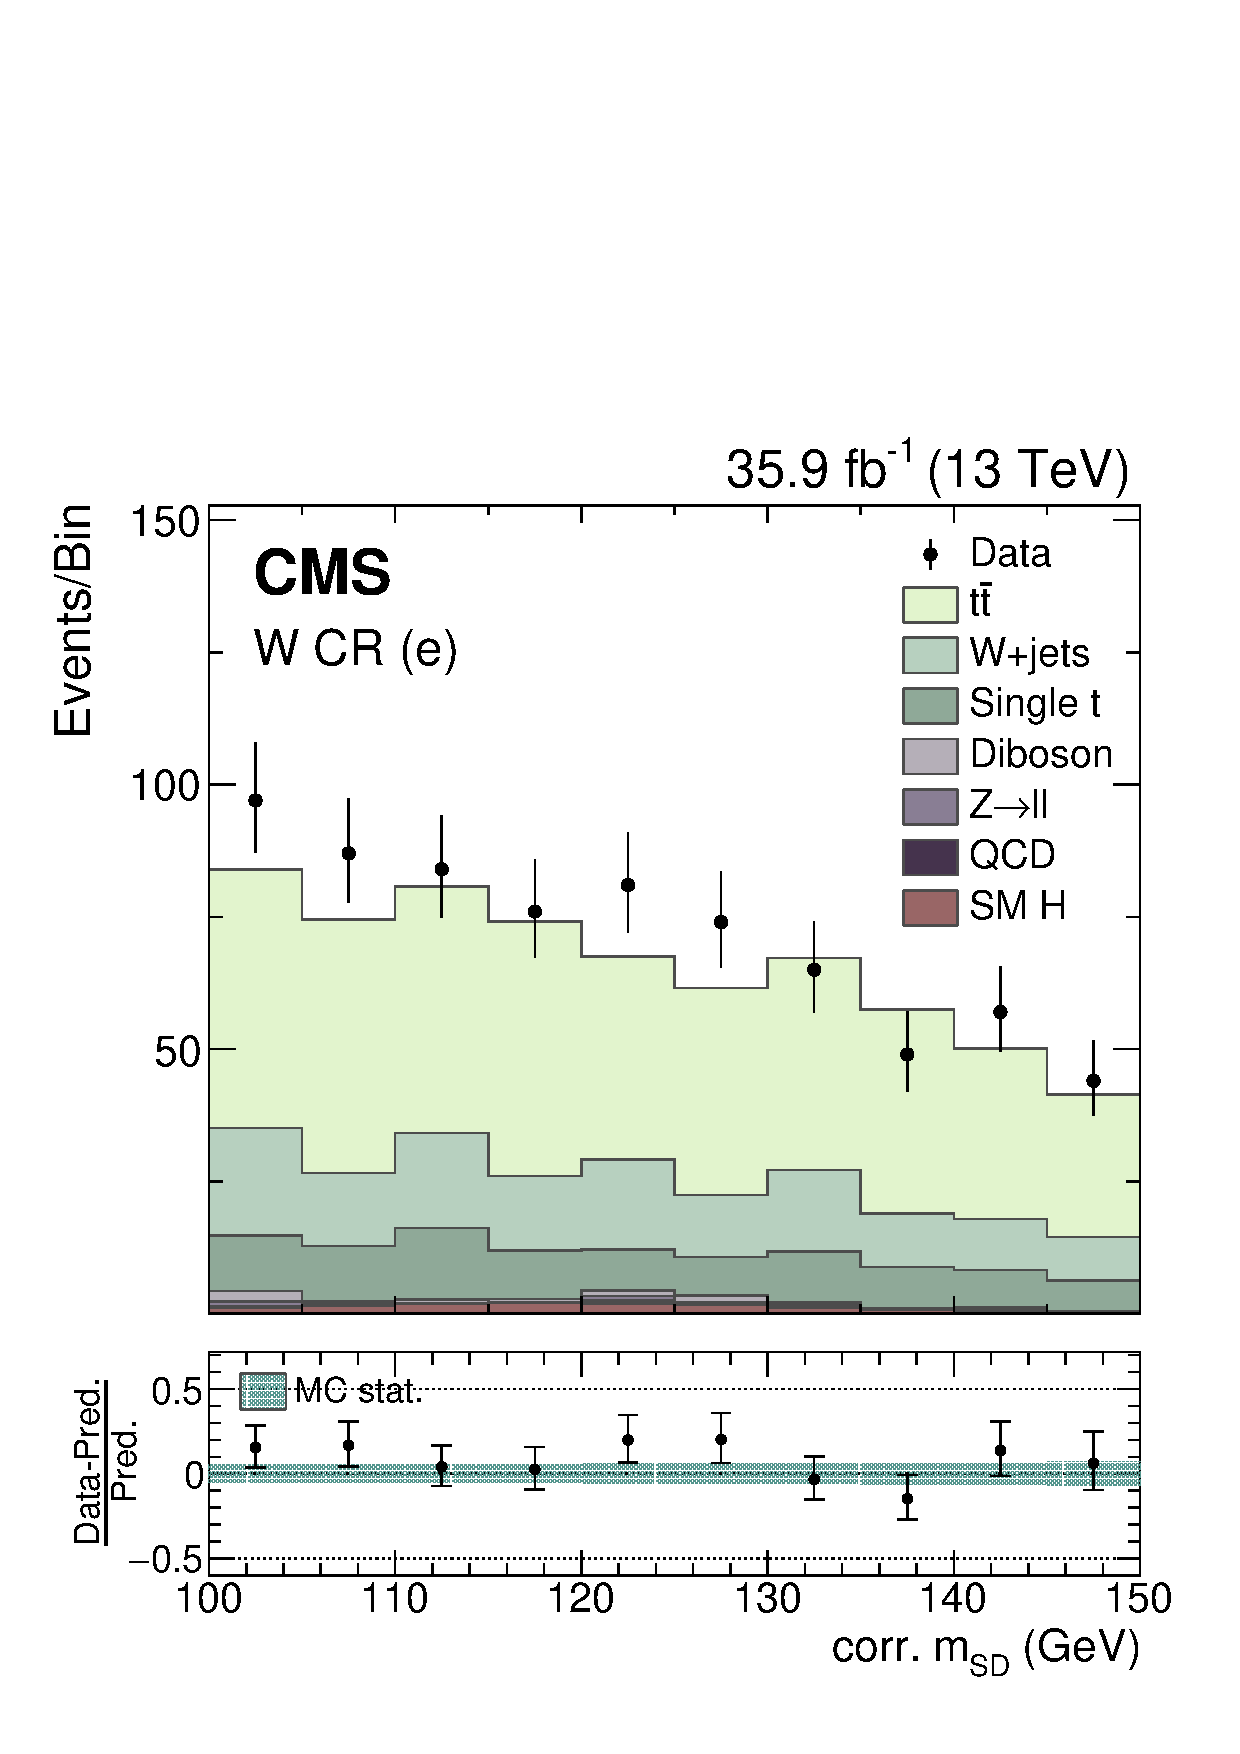
\includegraphics[width=0.4\textwidth]{figures/dataMC/cr_w_el_fj1MSD_corr.pdf}} \\
\caption{Prefit validation plots in the W CR (electron channel).}
\label{Fig_cr_w_el_1}
\end{figure}

\clearpage


\begin{figure}
\centering
 \subfloat{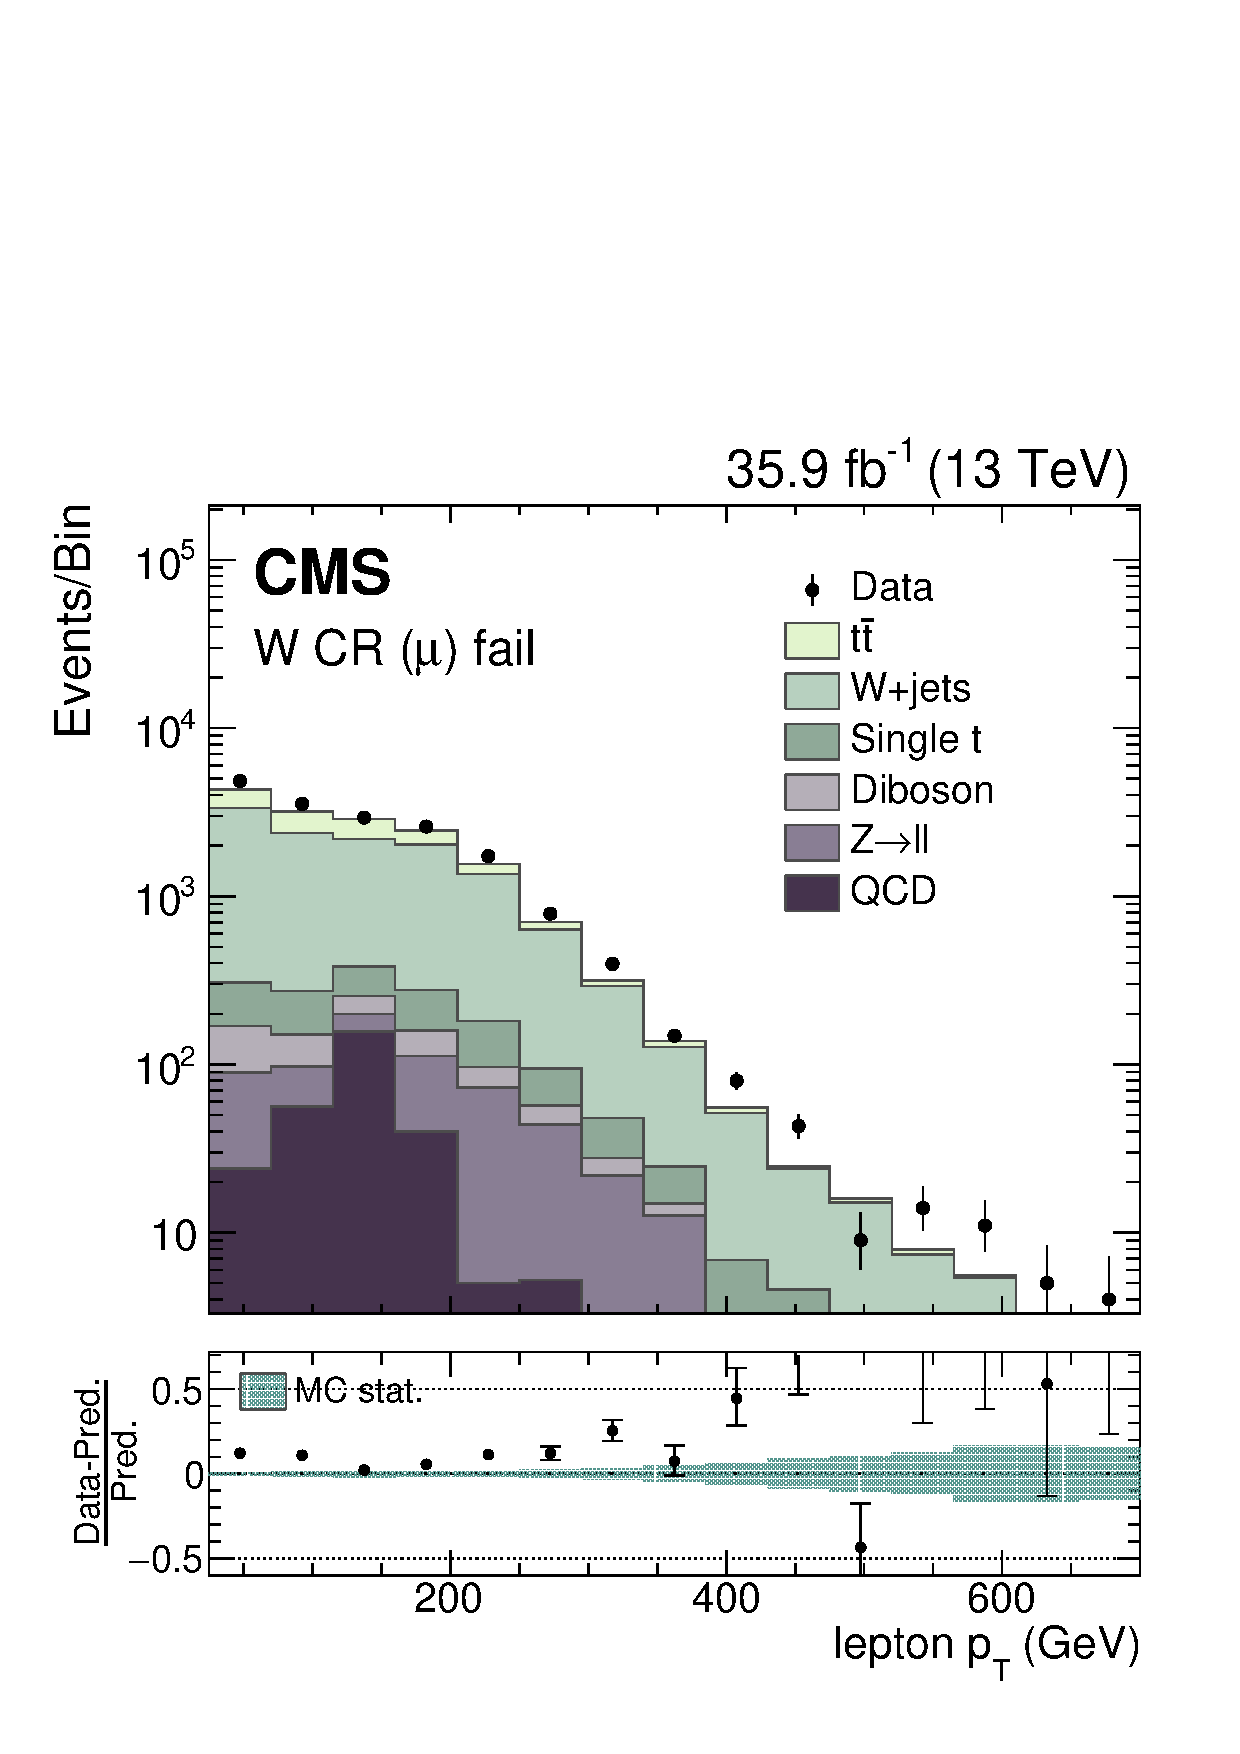
\includegraphics[width=0.4\textwidth]{figures/dataMC/cr_w_mu_fail_lep1Pt.pdf}}
 \subfloat{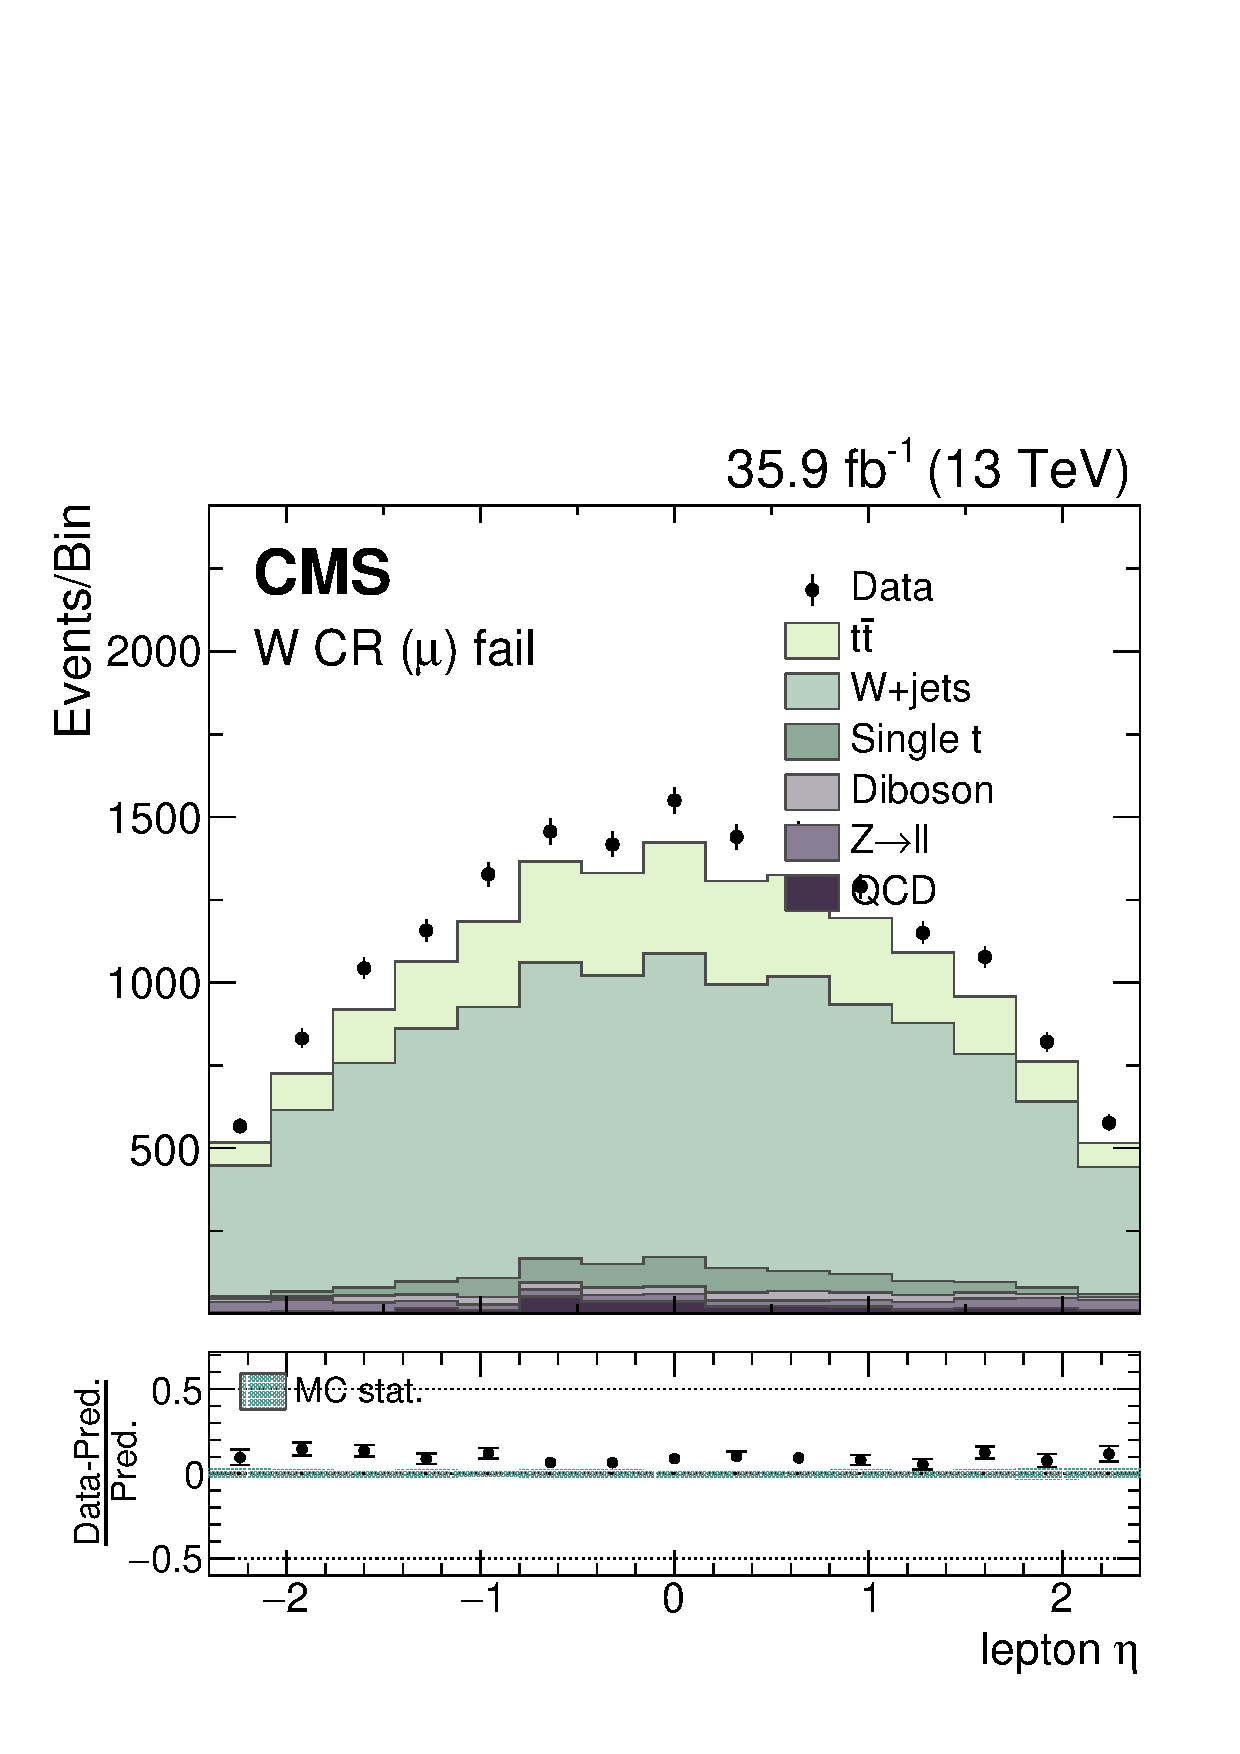
\includegraphics[width=0.4\textwidth]{figures/dataMC/cr_w_mu_fail_lep1Eta.pdf}} \\
 \subfloat{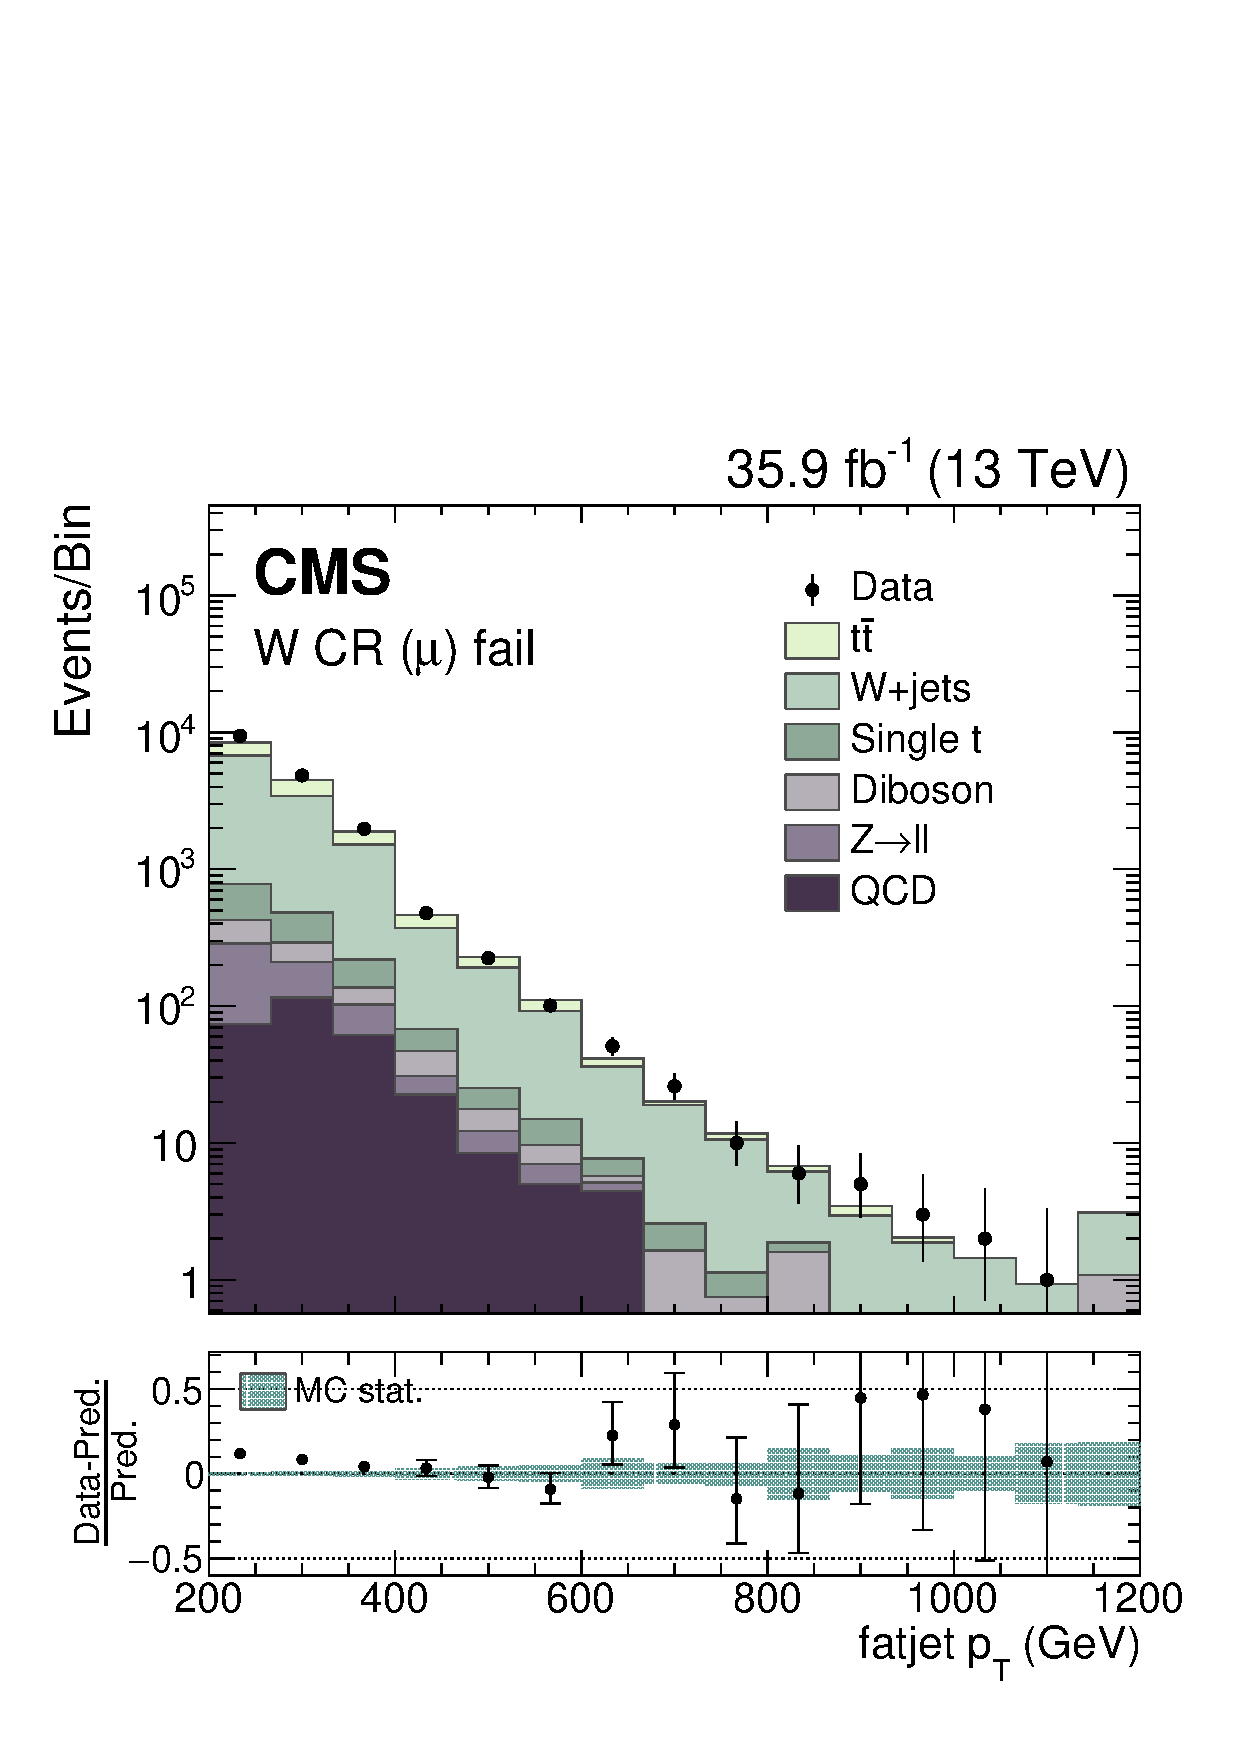
\includegraphics[width=0.4\textwidth]{figures/dataMC/cr_w_mu_fail_fj1Pt.pdf}}
 \subfloat{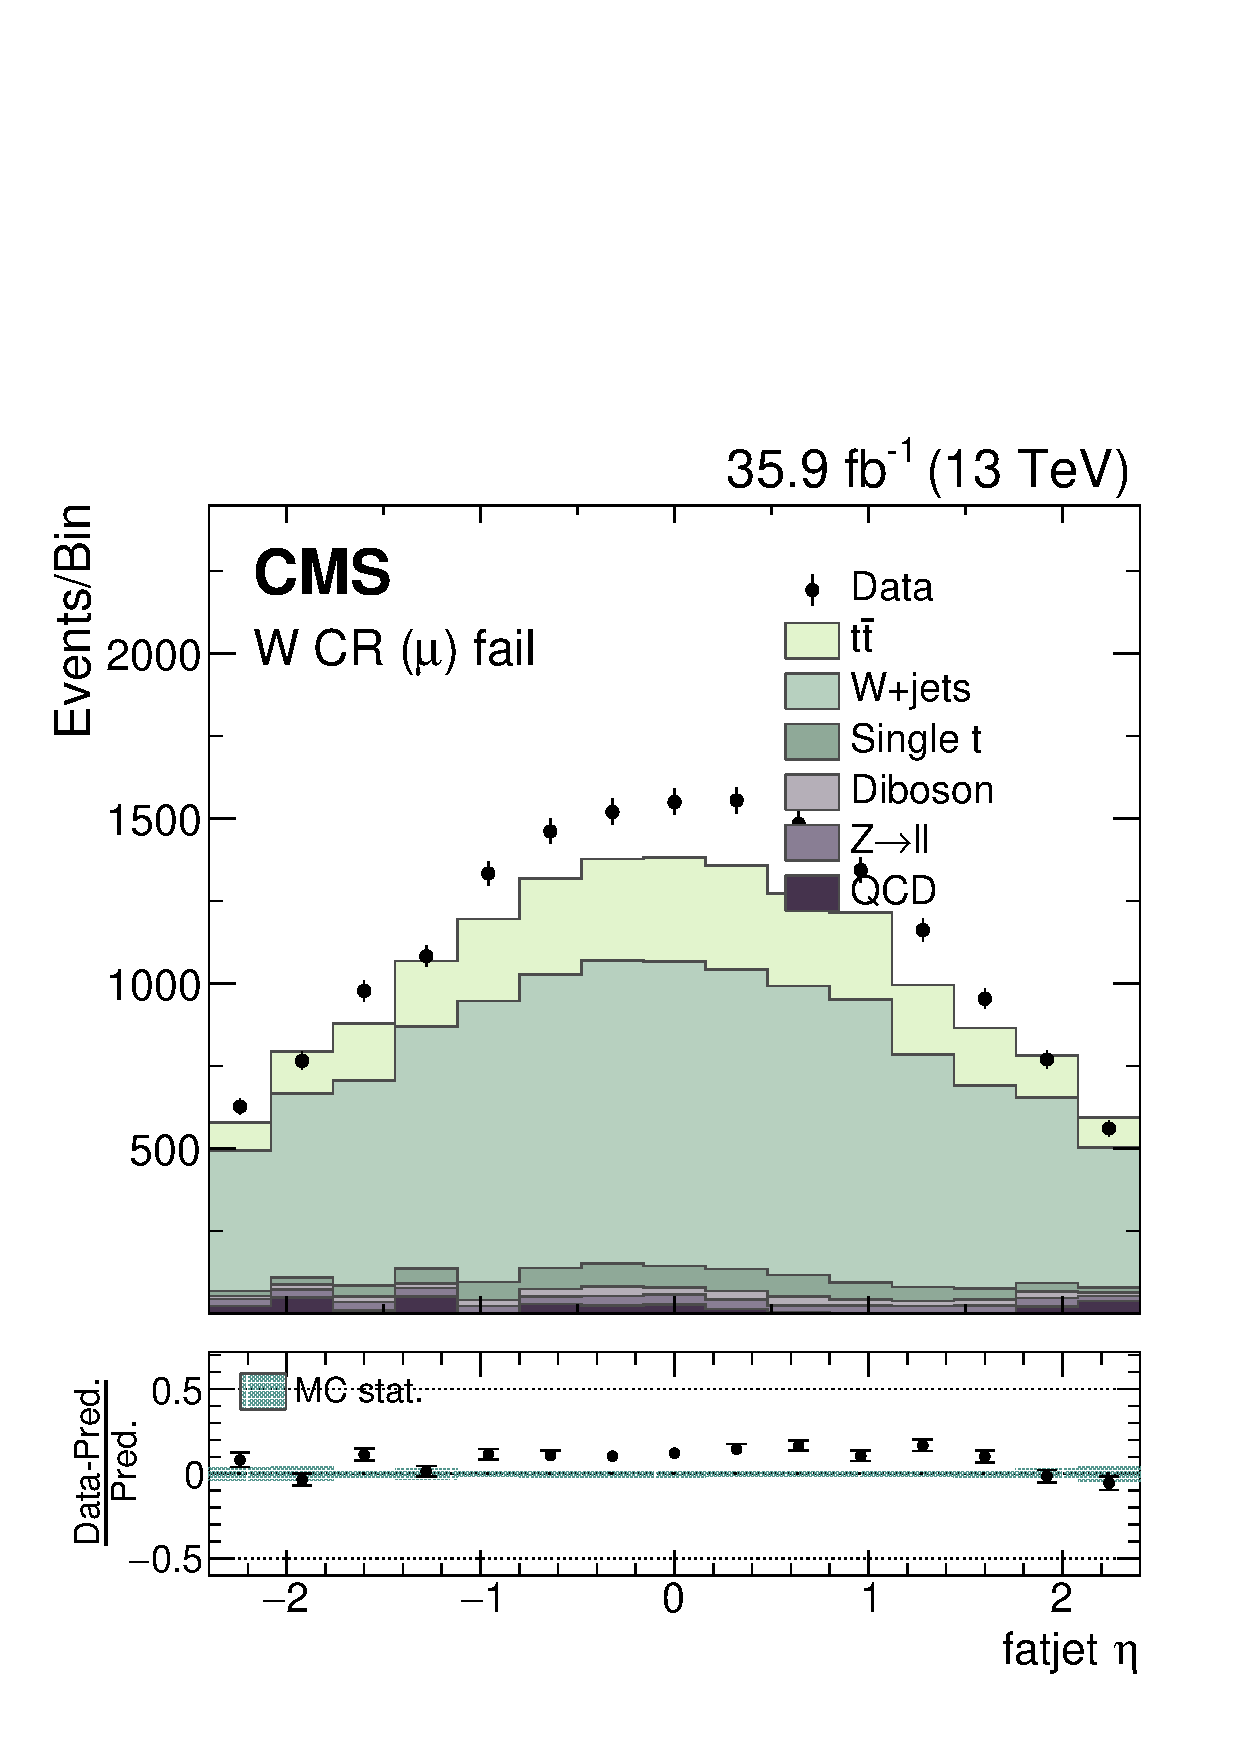
\includegraphics[width=0.4\textwidth]{figures/dataMC/cr_w_mu_fail_fj1Eta.pdf}} \\
 \subfloat{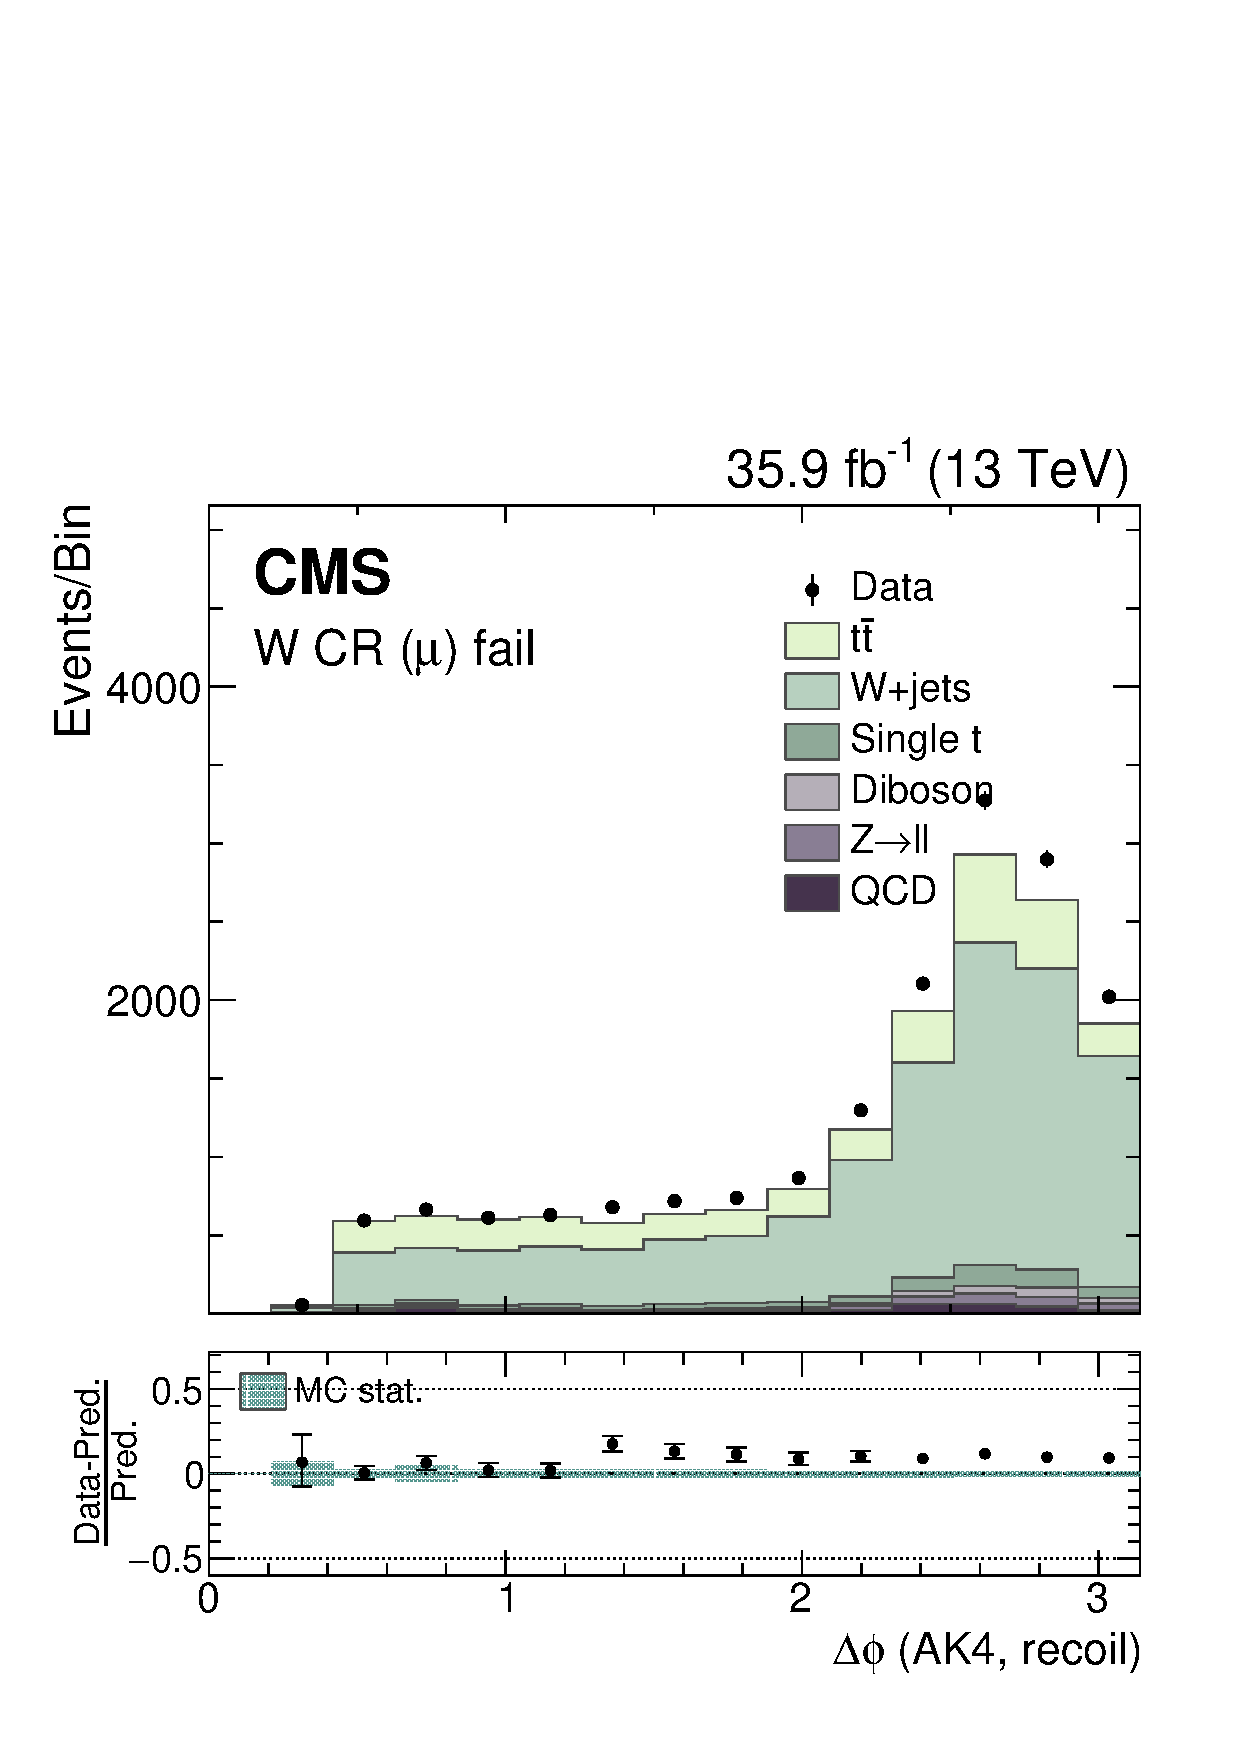
\includegraphics[width=0.4\textwidth]{figures/dataMC/cr_w_mu_fail_dphiUW.pdf}} 
 \subfloat{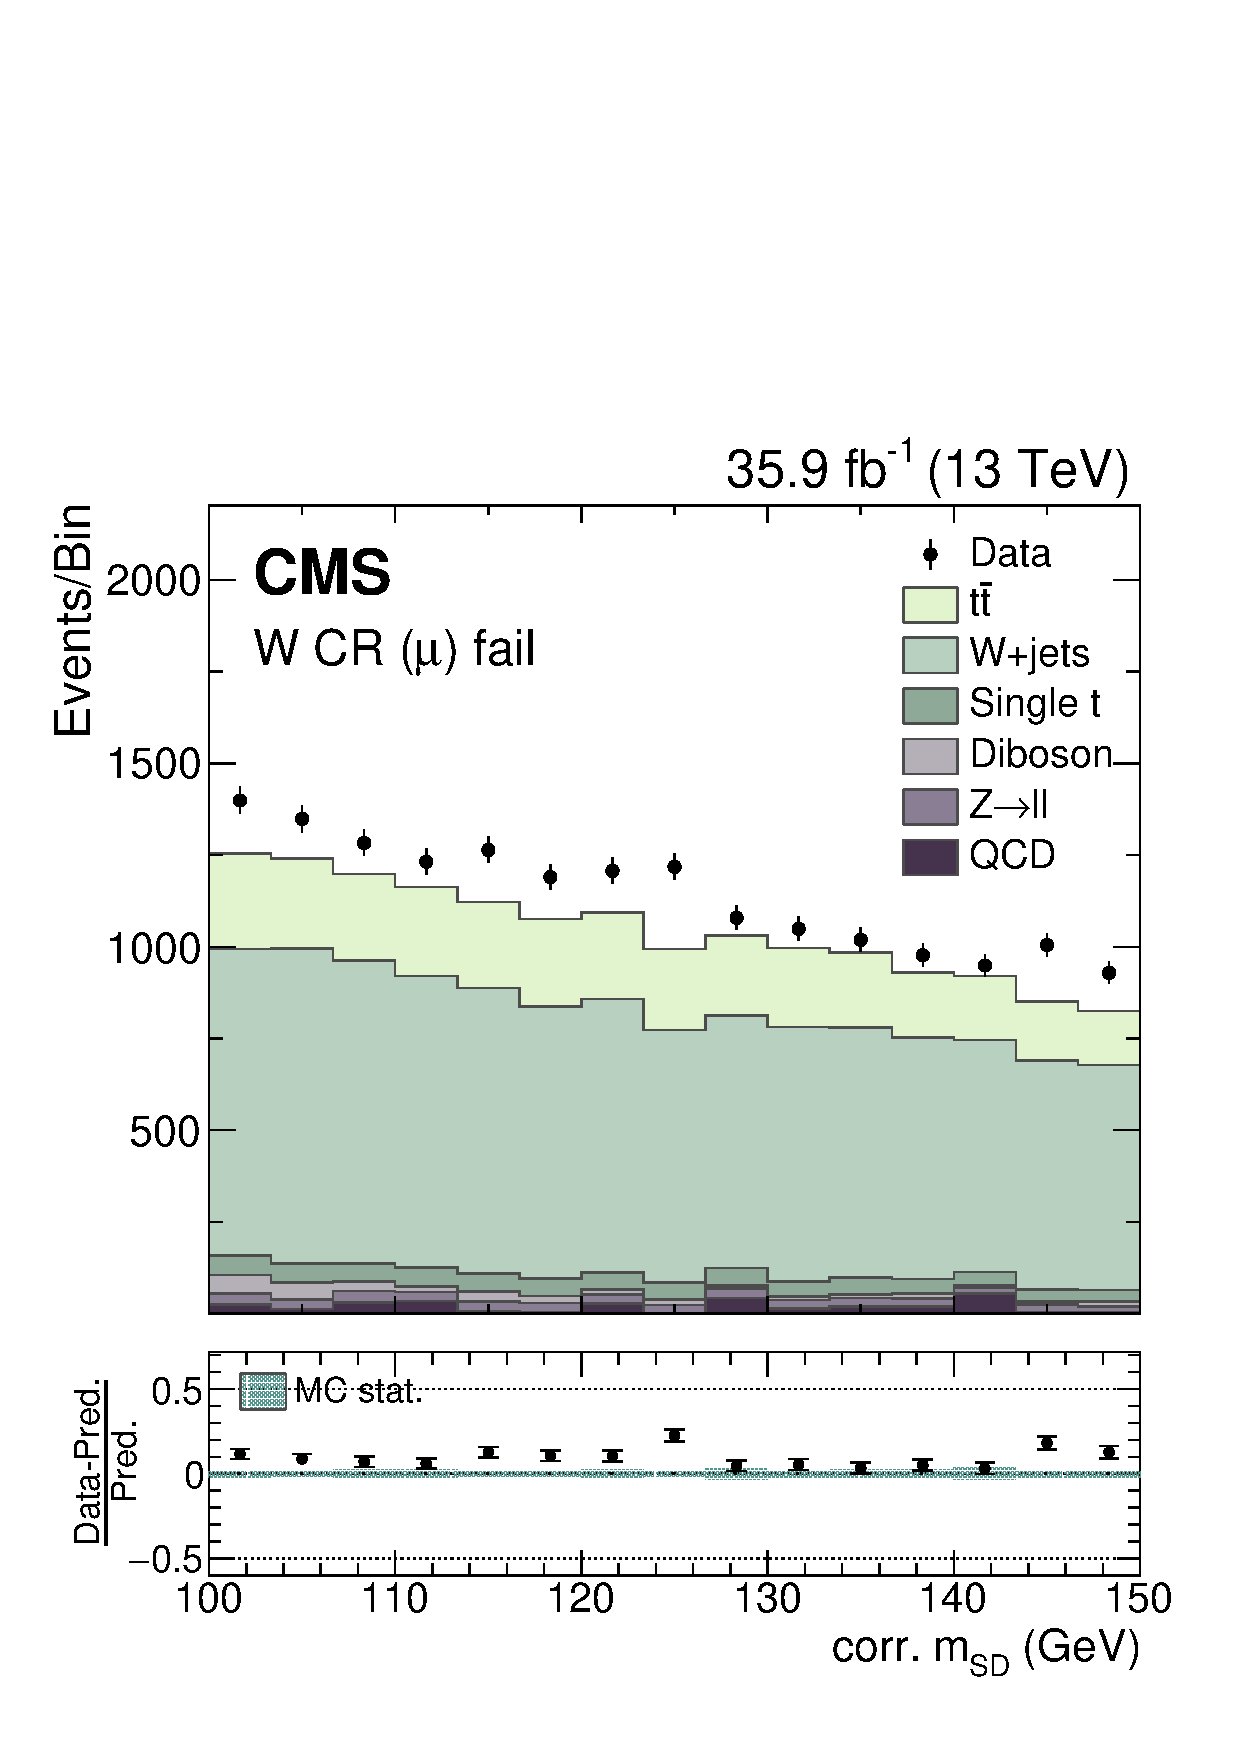
\includegraphics[width=0.4\textwidth]{figures/dataMC/cr_w_mu_fail_fj1MSD_corr.pdf}} \\
\caption{Prefit validation plots in the W fail CR (muon channel).}
\label{Fig_cr_w_mu_1}
\end{figure}

\clearpage


\begin{figure}
\centering
 \subfloat{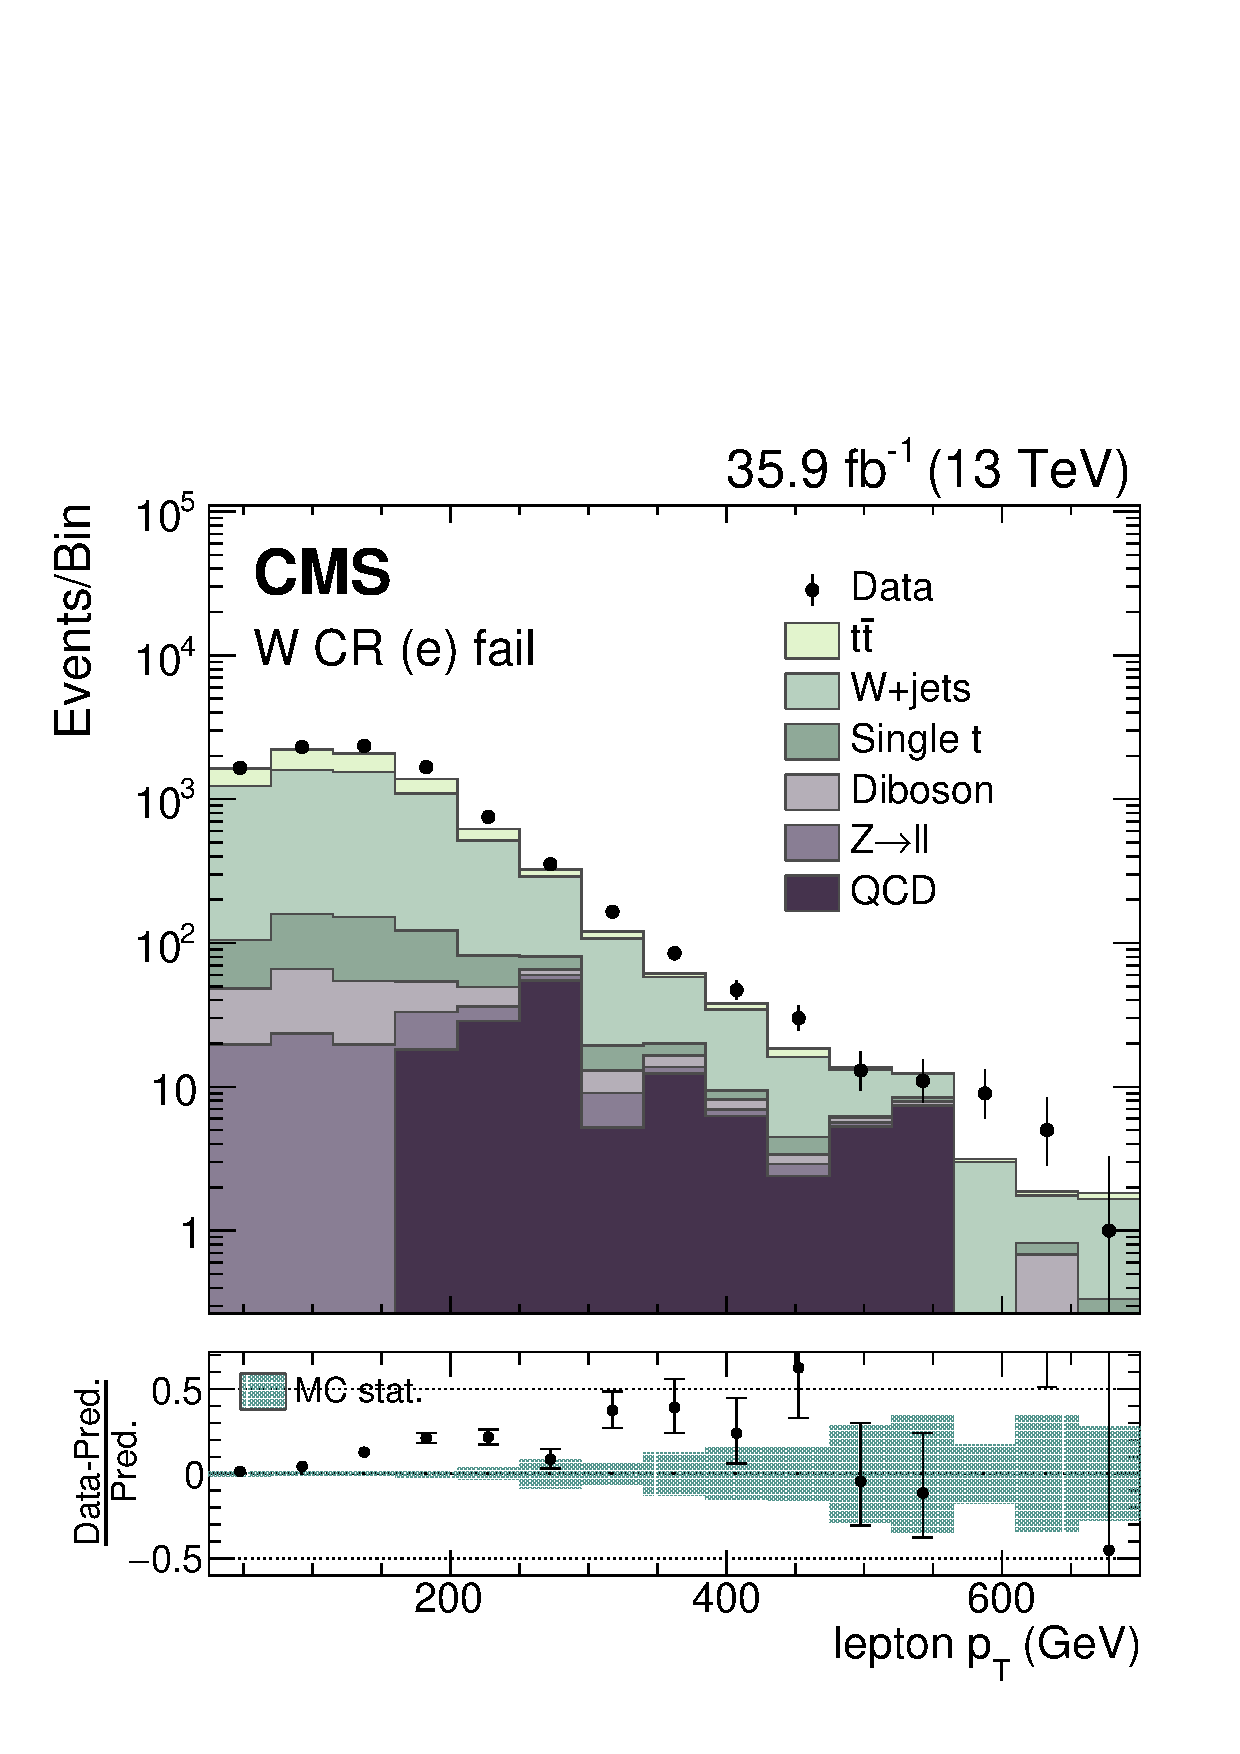
\includegraphics[width=0.4\textwidth]{figures/dataMC/cr_w_el_fail_lep1Pt.pdf}}
 \subfloat{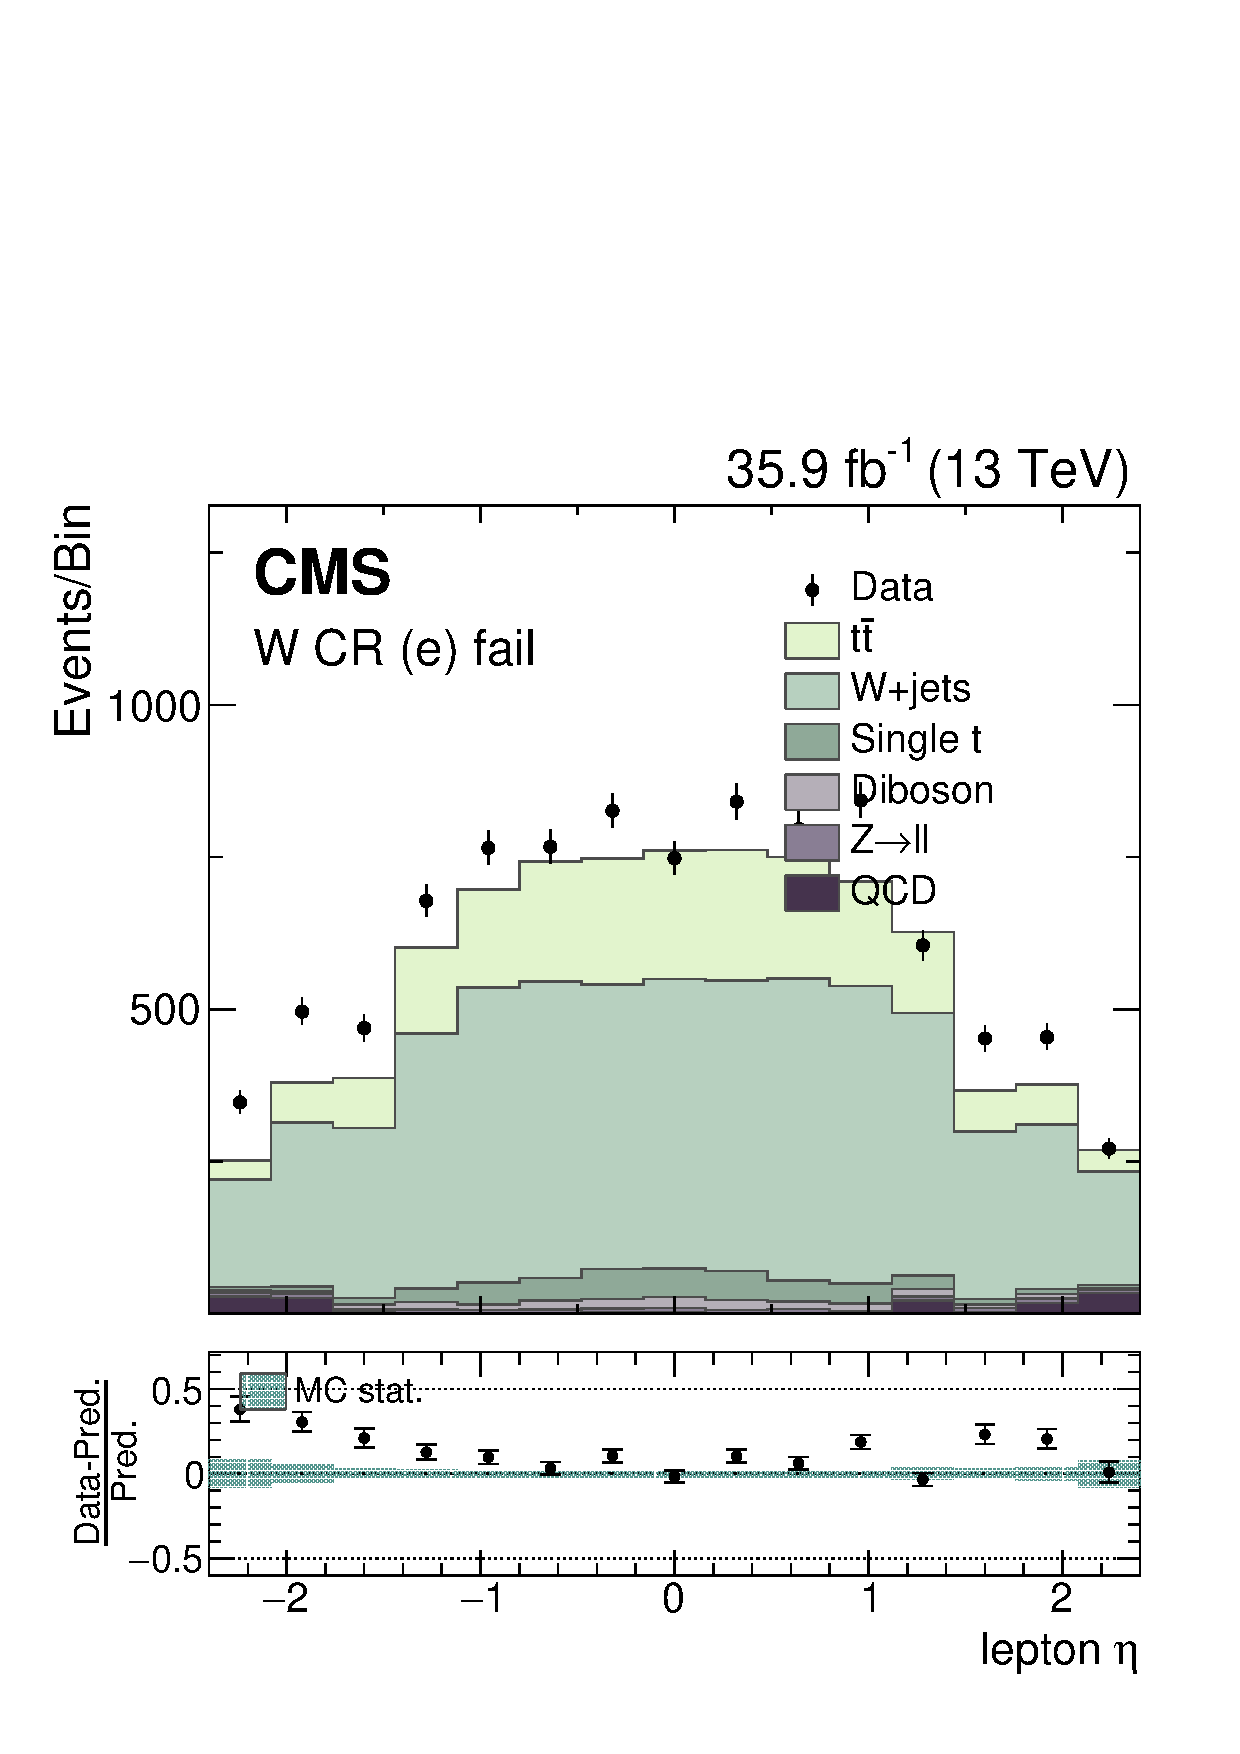
\includegraphics[width=0.4\textwidth]{figures/dataMC/cr_w_el_fail_lep1Eta.pdf}} \\
 \subfloat{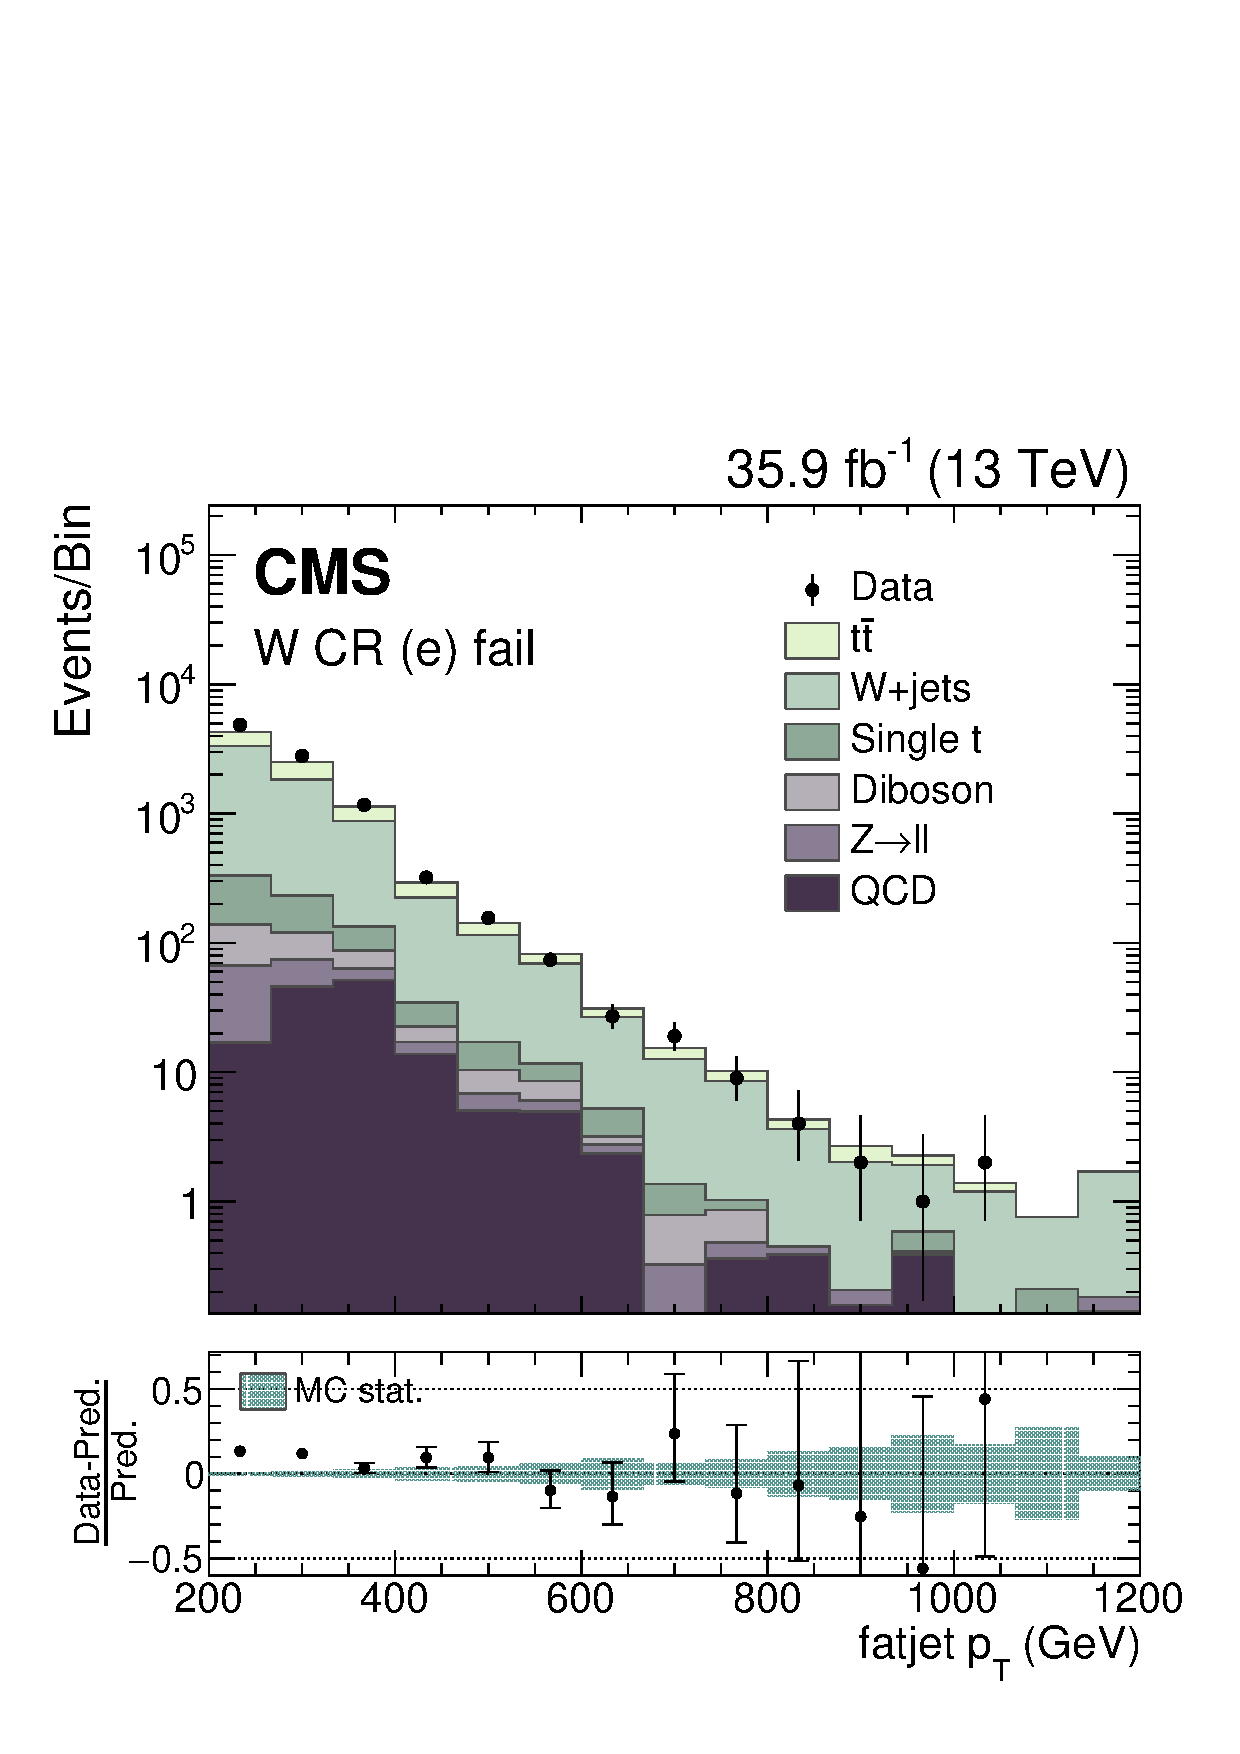
\includegraphics[width=0.4\textwidth]{figures/dataMC/cr_w_el_fail_fj1Pt.pdf}}
 \subfloat{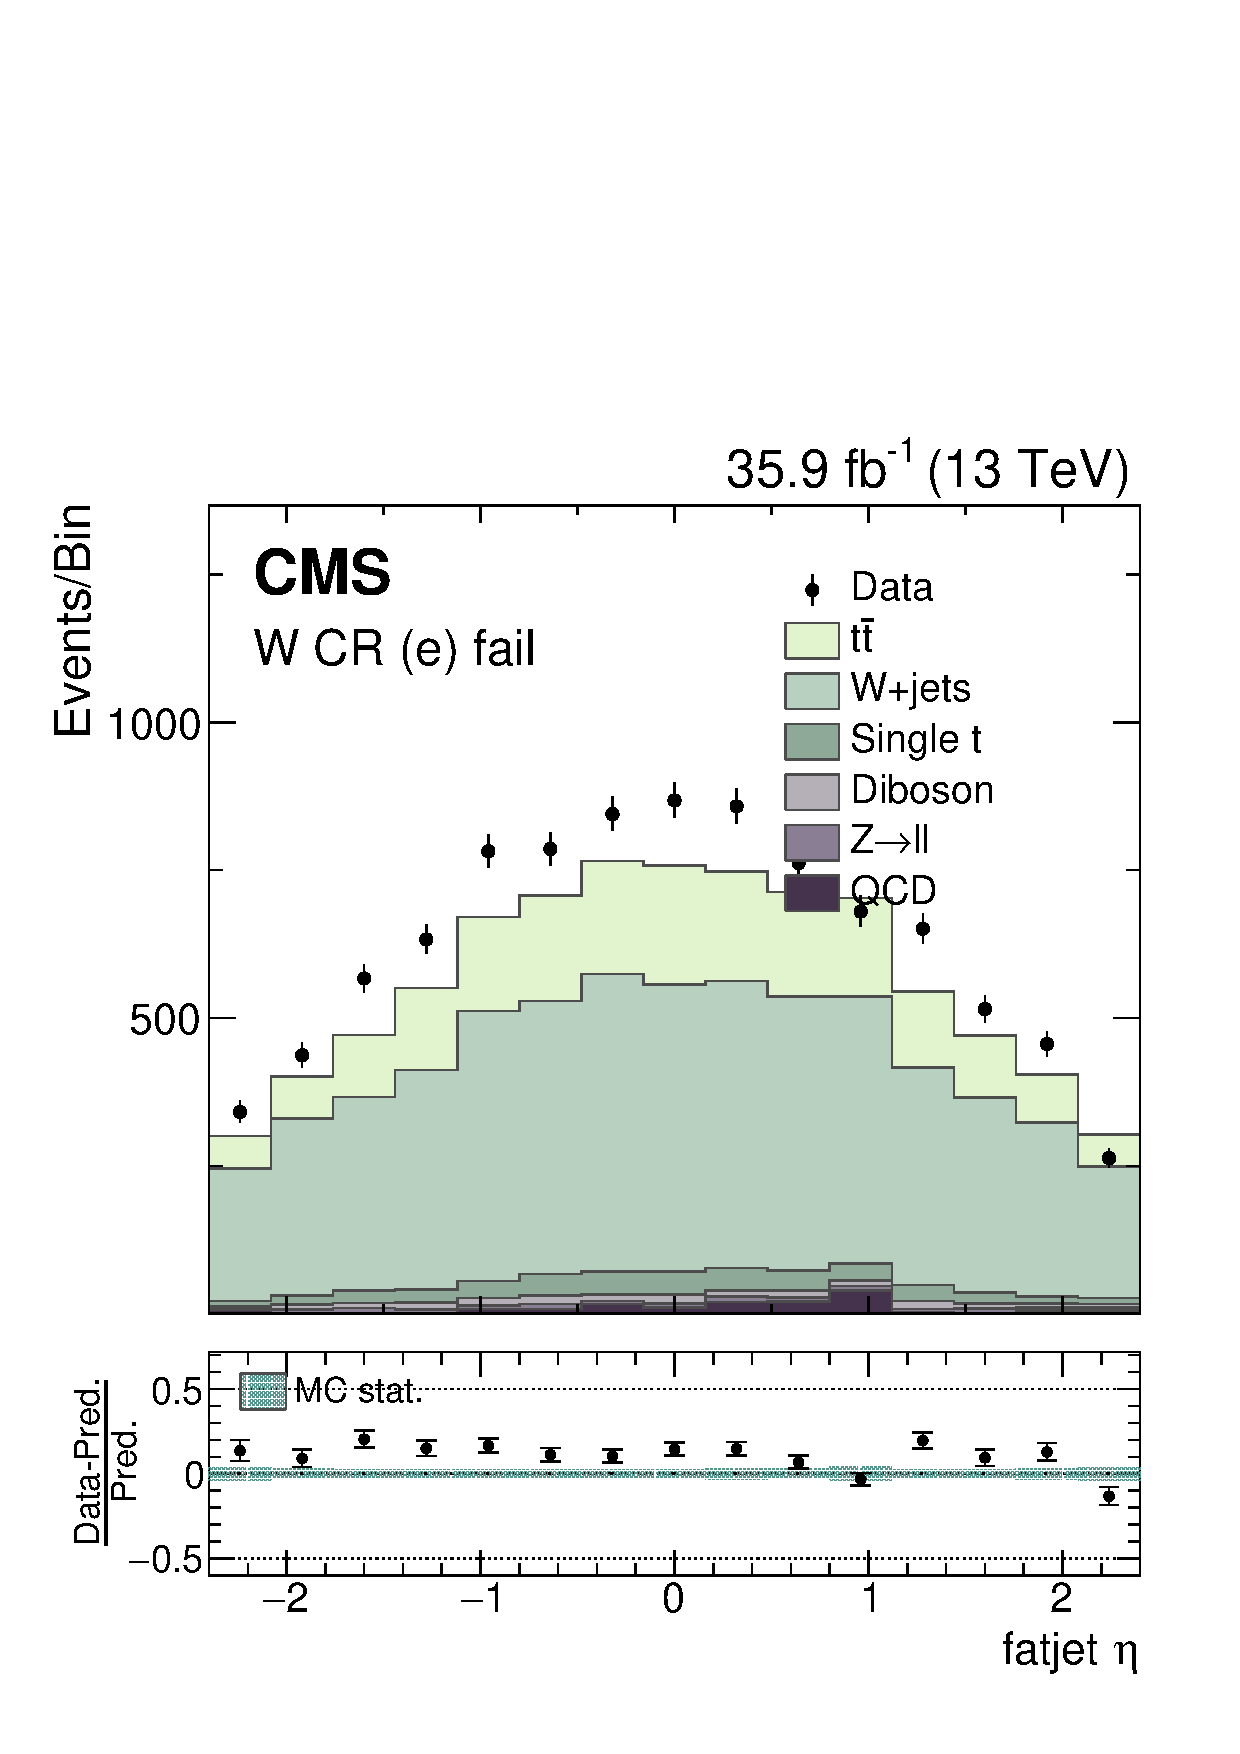
\includegraphics[width=0.4\textwidth]{figures/dataMC/cr_w_el_fail_fj1Eta.pdf}} \\
 \subfloat{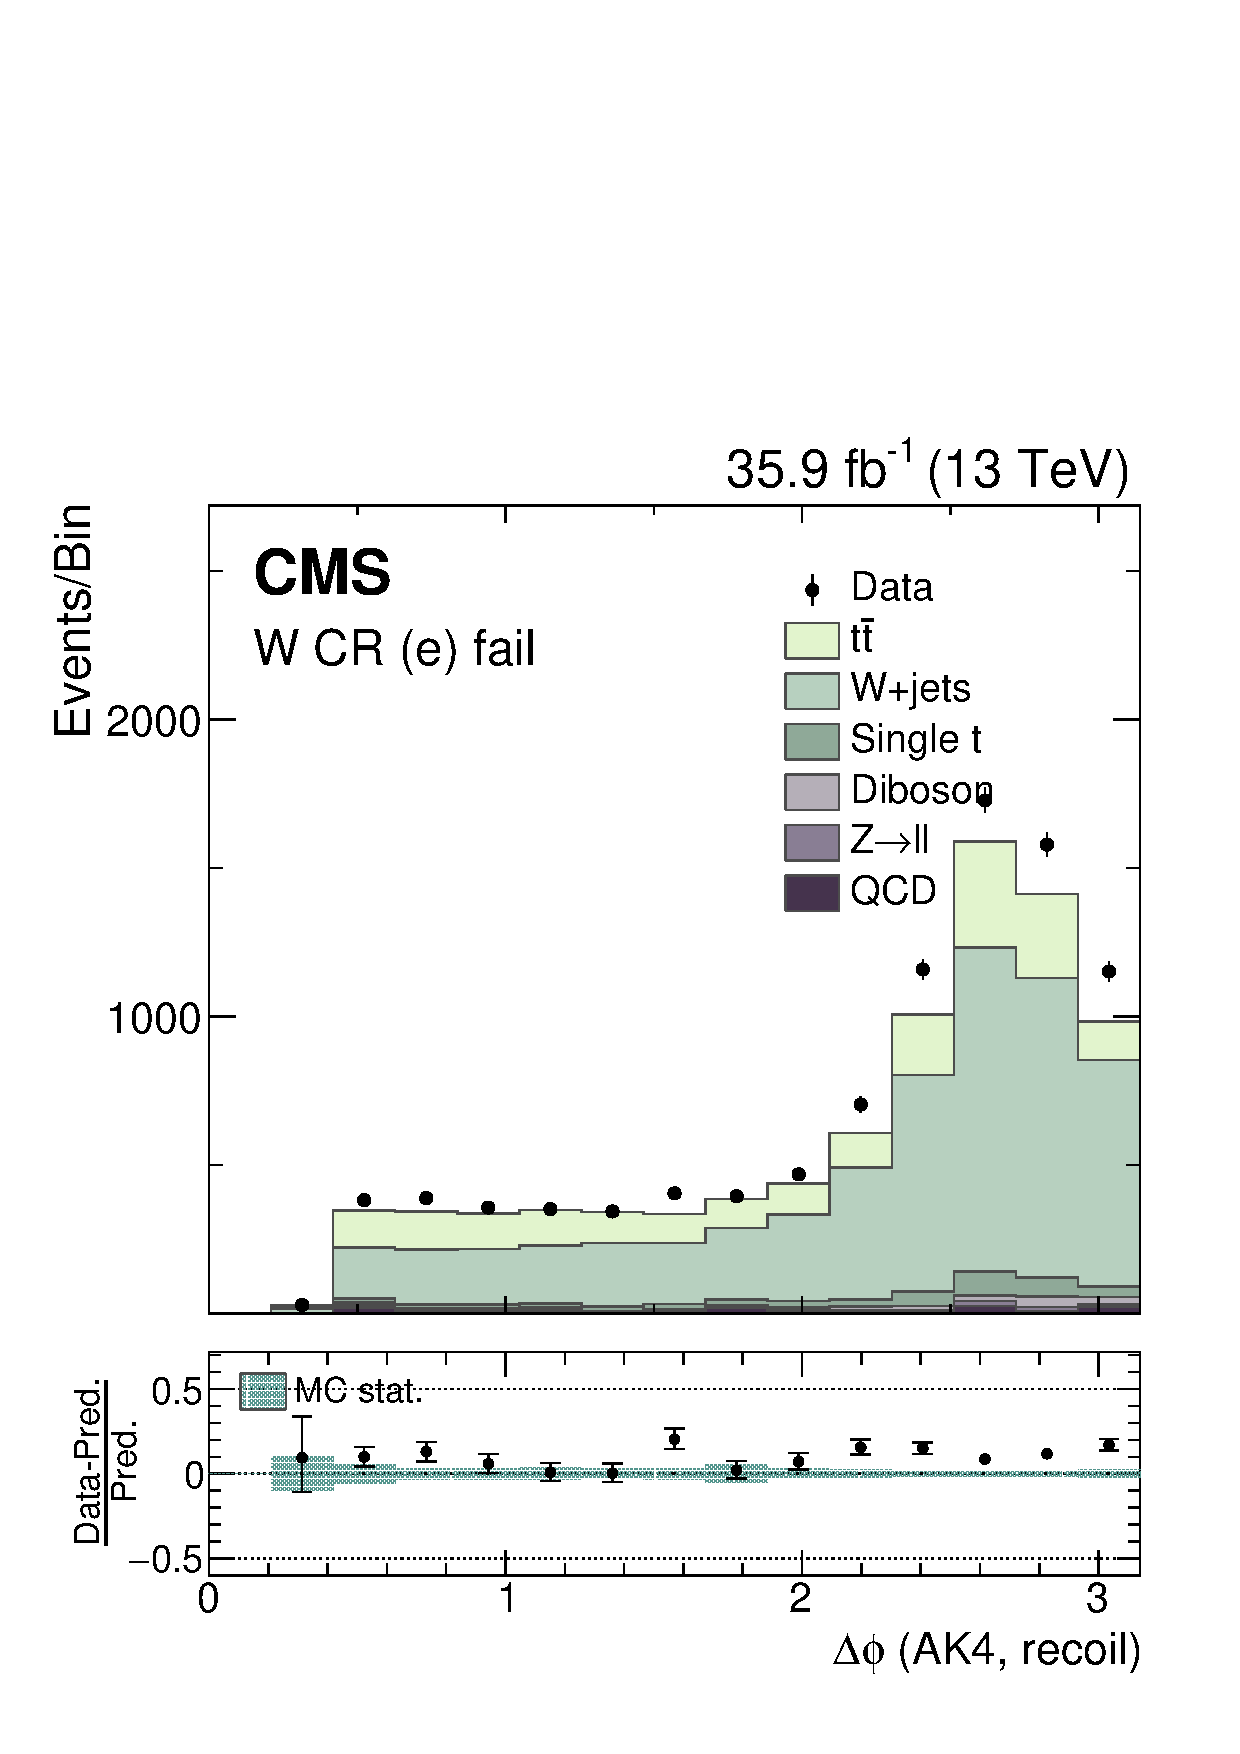
\includegraphics[width=0.4\textwidth]{figures/dataMC/cr_w_el_fail_dphiUW.pdf}} 
 \subfloat{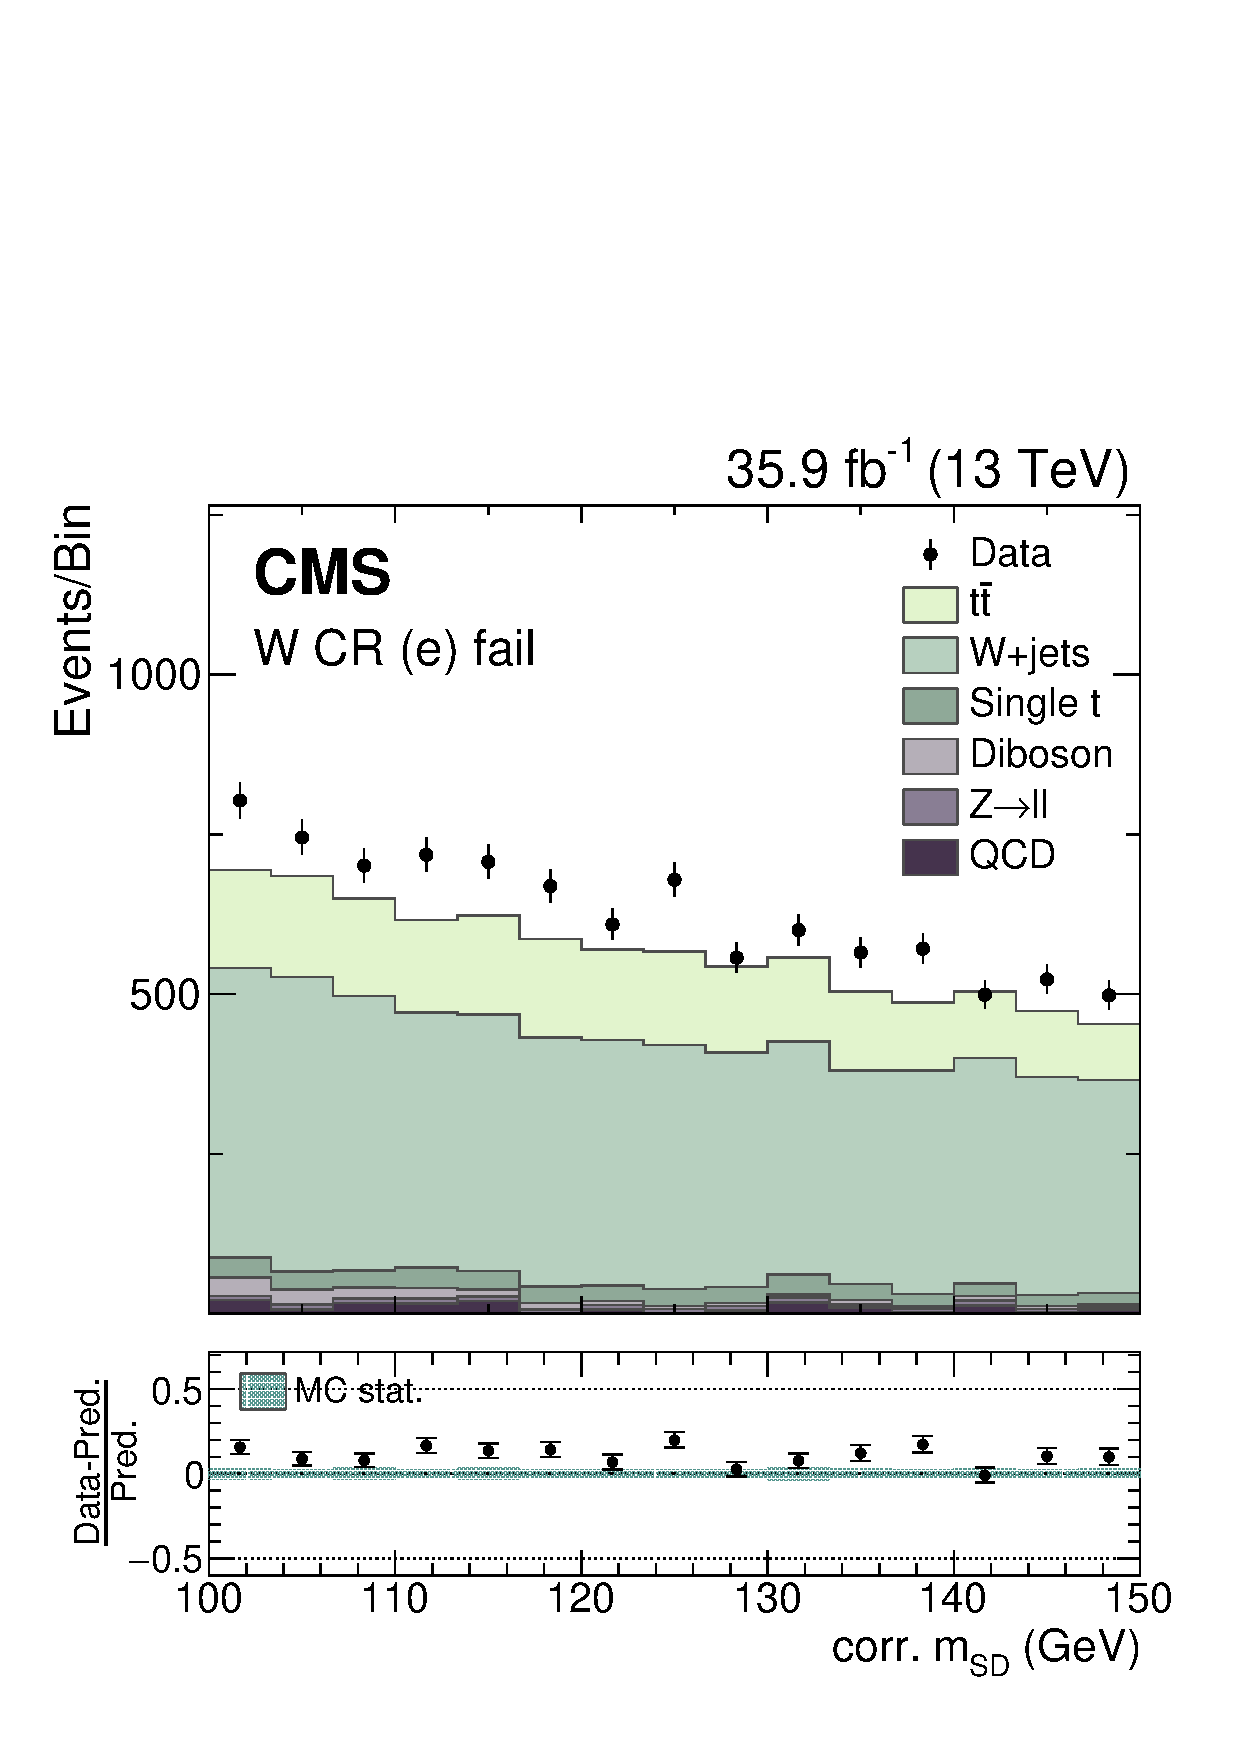
\includegraphics[width=0.4\textwidth]{figures/dataMC/cr_w_el_fail_fj1MSD_corr.pdf}} \\
\caption{Prefit validation plots in the W fail CR (electron channel).}
\label{Fig_cr_w_el_1}
\end{figure}

\clearpage

\begin{figure}
\centering
 \subfloat{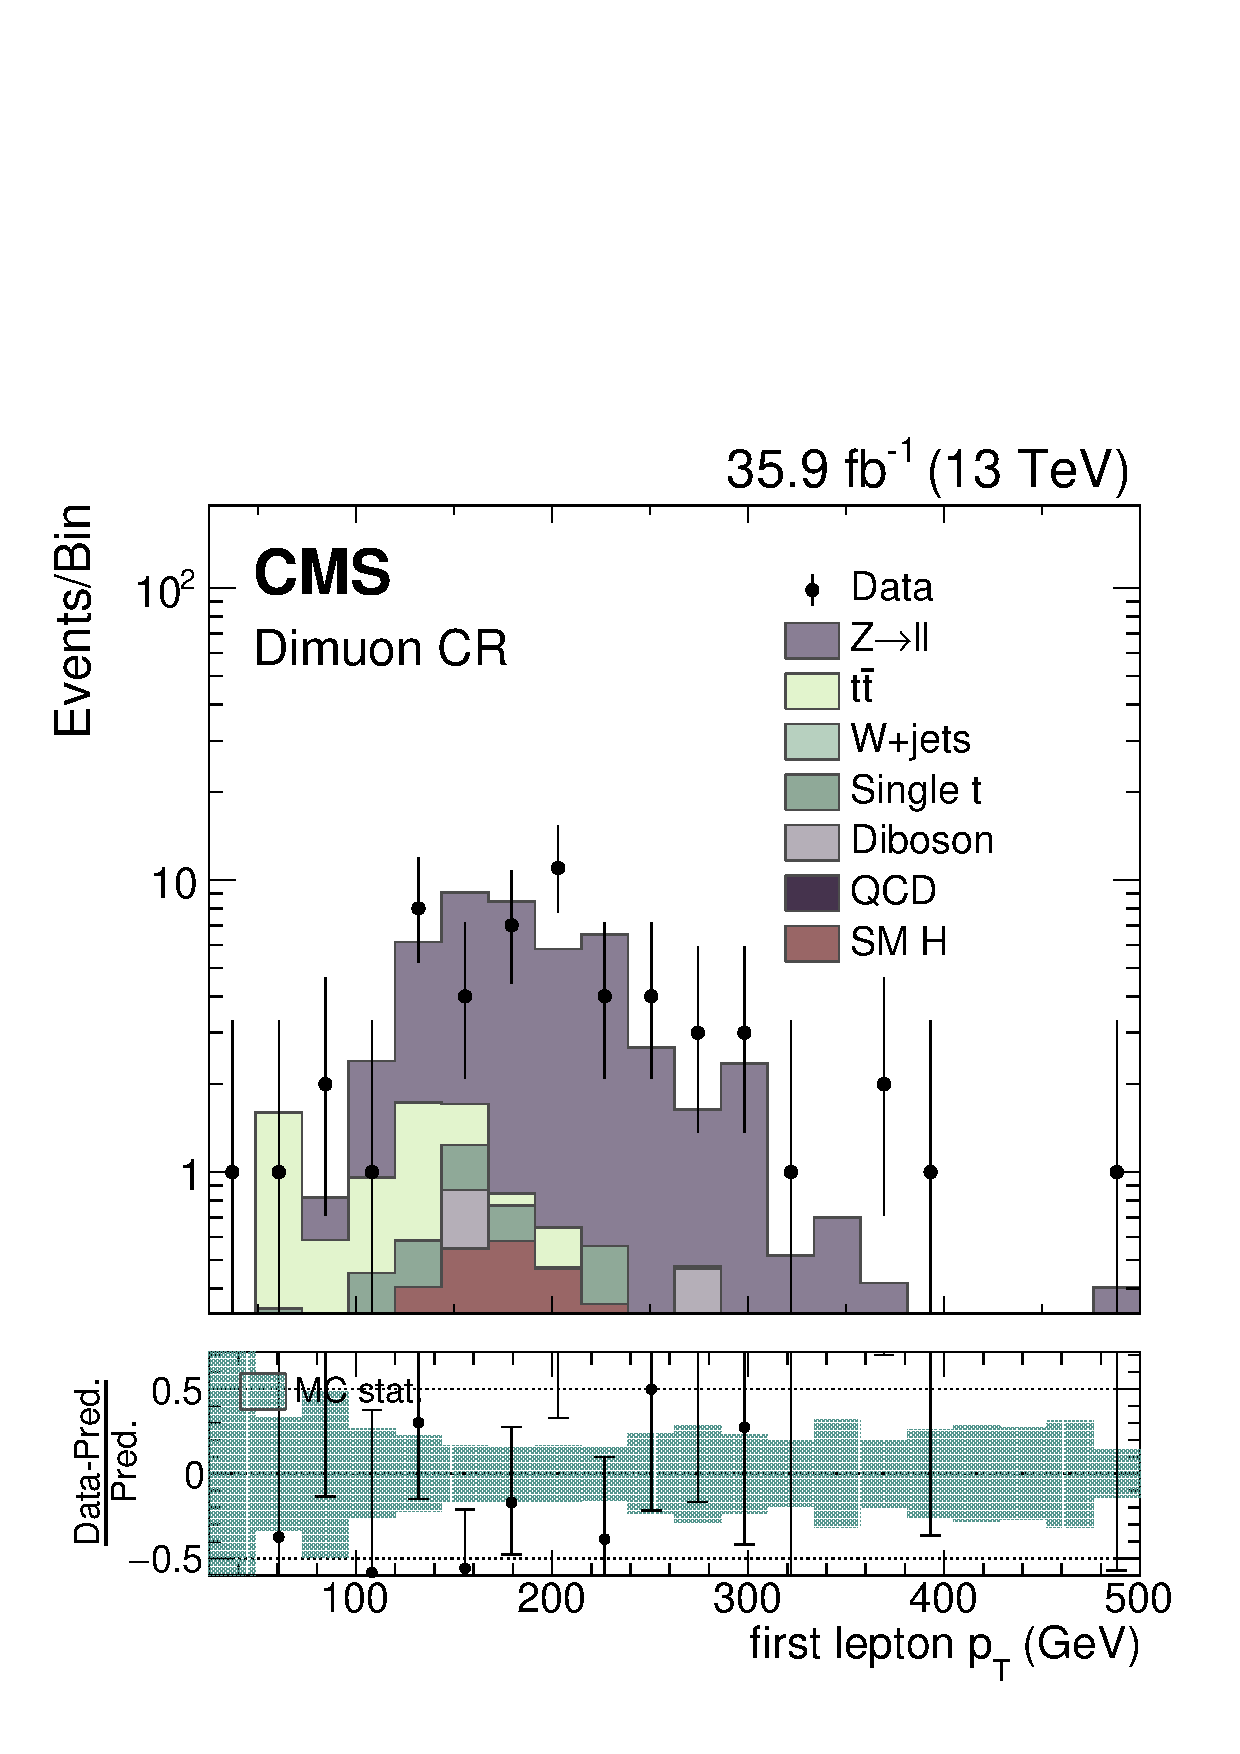
\includegraphics[width=0.4\textwidth]{figures/dataMC/cr_dimuon_lep1Pt.pdf}}
 \subfloat{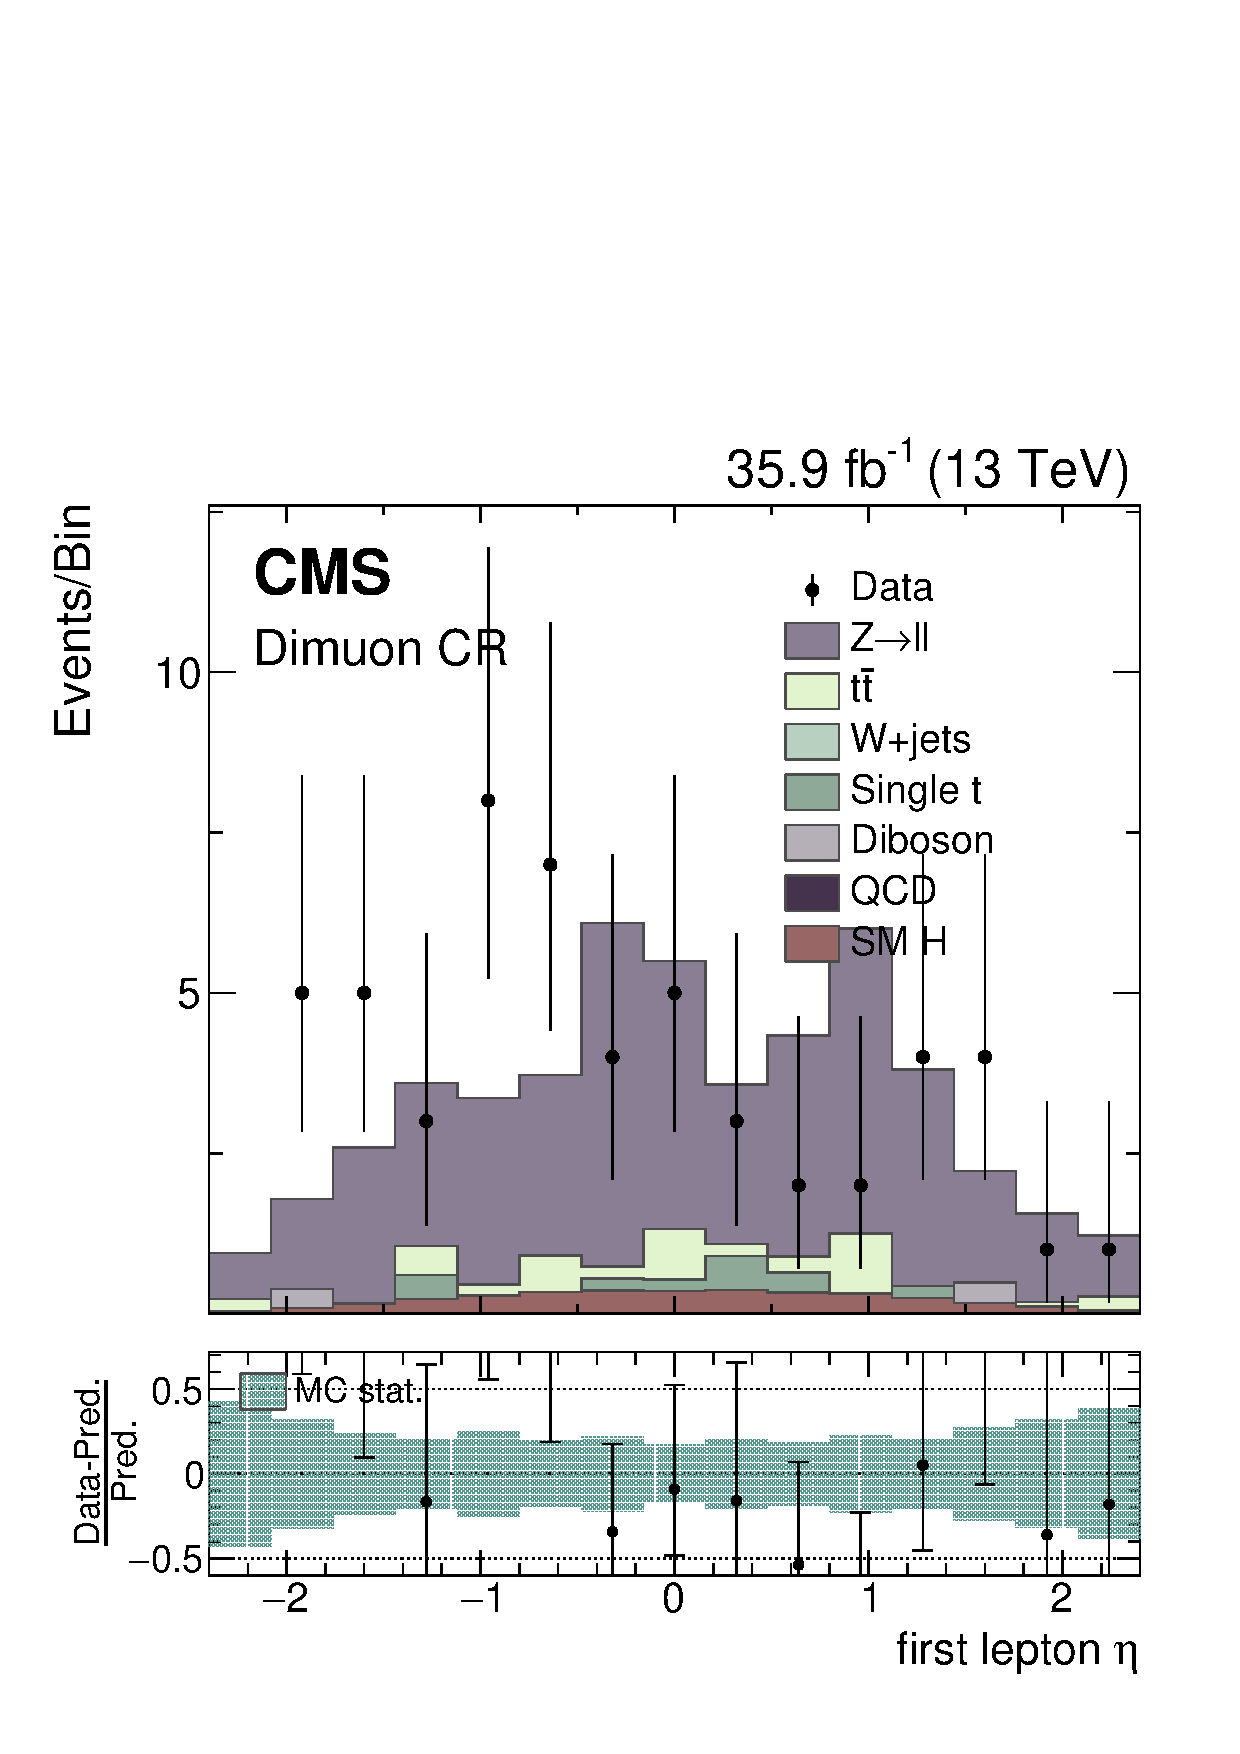
\includegraphics[width=0.4\textwidth]{figures/dataMC/cr_dimuon_lep1Eta.pdf}} \\
 \subfloat{\includegraphics[width=0.4\textwidth]{figures/dataMC/cr_dimuon_fj1Pt.pdf}}
 \subfloat{\includegraphics[width=0.4\textwidth]{figures/dataMC/cr_dimuon_fj1Eta.pdf}} \\
 \subfloat{\includegraphics[width=0.4\textwidth]{figures/dataMC/cr_dimuon_dphiUZ.pdf}} 
 \subfloat{\includegraphics[width=0.4\textwidth]{figures/dataMC/cr_dimuon_fj1MSD_corr.pdf}} \\
\caption{Prefit validation plots in the dimuon CR.}
\label{Fig_cr_dimuon_1}
\end{figure}

\clearpage


\begin{figure}
\centering
 \subfloat{\includegraphics[width=0.4\textwidth]{figures/dataMC/cr_dielectron_lep1Pt.pdf}}
 \subfloat{\includegraphics[width=0.4\textwidth]{figures/dataMC/cr_dielectron_lep1Eta.pdf}} \\
 \subfloat{\includegraphics[width=0.4\textwidth]{figures/dataMC/cr_dielectron_fj1Pt.pdf}}
 \subfloat{\includegraphics[width=0.4\textwidth]{figures/dataMC/cr_dielectron_fj1Eta.pdf}} \\
 \subfloat{\includegraphics[width=0.4\textwidth]{figures/dataMC/cr_dielectron_dphiUZ.pdf}} 
 \subfloat{\includegraphics[width=0.4\textwidth]{figures/dataMC/cr_dielectron_fj1MSD_corr.pdf}} \\
\caption{Prefit validation plots in the dielectron CR.}
\label{Fig_cr_dielectron_1}
\end{figure}

\clearpage

\begin{figure}
\centering
 \subfloat{\includegraphics[width=0.4\textwidth]{figures/dataMC/cr_dimuon_fail_lep1Pt.pdf}}
 \subfloat{\includegraphics[width=0.4\textwidth]{figures/dataMC/cr_dimuon_fail_lep1Eta.pdf}} \\
 \subfloat{\includegraphics[width=0.4\textwidth]{figures/dataMC/cr_dimuon_fail_fj1Pt.pdf}}
 \subfloat{\includegraphics[width=0.4\textwidth]{figures/dataMC/cr_dimuon_fail_fj1Eta.pdf}} \\
 \subfloat{\includegraphics[width=0.4\textwidth]{figures/dataMC/cr_dimuon_fail_dphiUZ.pdf}} 
 \subfloat{\includegraphics[width=0.4\textwidth]{figures/dataMC/cr_dimuon_fail_fj1MSD_corr.pdf}} \\
\caption{Prefit validation plots in the dimuon fail CR.}
\label{Fig_cr_dimuon_1}
\end{figure}

\clearpage


\begin{figure}
\centering
 \subfloat{\includegraphics[width=0.4\textwidth]{figures/dataMC/cr_dielectron_fail_lep1Pt.pdf}}
 \subfloat{\includegraphics[width=0.4\textwidth]{figures/dataMC/cr_dielectron_fail_lep1Eta.pdf}} \\
 \subfloat{\includegraphics[width=0.4\textwidth]{figures/dataMC/cr_dielectron_fail_fj1Pt.pdf}}
 \subfloat{\includegraphics[width=0.4\textwidth]{figures/dataMC/cr_dielectron_fail_fj1Eta.pdf}} \\
 \subfloat{\includegraphics[width=0.4\textwidth]{figures/dataMC/cr_dielectron_fail_dphiUZ.pdf}} 
 \subfloat{\includegraphics[width=0.4\textwidth]{figures/dataMC/cr_dielectron_fail_fj1MSD_corr.pdf}} \\
\caption{Prefit validation plots in the dielectron fail CR.}
\label{Fig_cr_dielectron_1}
\end{figure}

\clearpage


\begin{figure}
\centering
 \subfloat{\includegraphics[width=0.4\textwidth]{figures/dataMC/cr_ttbar_mu_RecoilUW2.pdf}} 
 \subfloat{\includegraphics[width=0.4\textwidth]{figures/dataMC/cr_ttbar_el_RecoilUW2.pdf}} \\
 \subfloat{\includegraphics[width=0.4\textwidth]{figures/dataMC/cr_w_mu_RecoilUW2.pdf}} 
 \subfloat{\includegraphics[width=0.4\textwidth]{figures/dataMC/cr_w_el_RecoilUW2.pdf}} \\
 \subfloat{\includegraphics[width=0.4\textwidth]{figures/dataMC/cr_dimuon_RecoilUZ2.pdf}} 
 \subfloat{\includegraphics[width=0.4\textwidth]{figures/dataMC/cr_dielectron_RecoilUZ2.pdf}} \\
\caption{Prefit validation plots in the six CR regions with passing double-b cut.}
\label{Fig_cr_Recoil}
\end{figure}




\clearpage


\begin{figure}
\centering
 \subfloat{\includegraphics[width=0.4\textwidth]{figures/dataMC/cr_ttbar_mu_fail_RecoilUW2.pdf}} 
 \subfloat{\includegraphics[width=0.4\textwidth]{figures/dataMC/cr_ttbar_el_fail_RecoilUW2.pdf}} \\
 \subfloat{\includegraphics[width=0.4\textwidth]{figures/dataMC/cr_w_mu_fail_RecoilUW2.pdf}} 
 \subfloat{\includegraphics[width=0.4\textwidth]{figures/dataMC/cr_w_el_fail_RecoilUW2.pdf}} \\
 \subfloat{\includegraphics[width=0.4\textwidth]{figures/dataMC/cr_dimuon_fail_RecoilUZ2.pdf}} 
 \subfloat{\includegraphics[width=0.4\textwidth]{figures/dataMC/cr_dielectron_fail_RecoilUZ2.pdf}} \\
\caption{Prefit validation plots in the six CR regions with failing double-b cut.}
\label{Fig_cr_Recoil_fail}
\end{figure}

\begin{figure}
\centering
 \subfloat{\includegraphics[width=0.45\textwidth]{figures/dataMC/sr_MET2.pdf}} 
 \subfloat{\includegraphics[width=0.45\textwidth]{figures/dataMC/sr_puppimet.pdf}} \\
 \subfloat{\includegraphics[width=0.45\textwidth]{figures/dataMC/cr_znunu_MET2.pdf}} 
 \subfloat{\includegraphics[width=0.45\textwidth]{figures/dataMC/cr_znunu_puppimet.pdf}} \\
\caption{Upper row: prefit MET distribution in the signal region in three different binnings. The upper left figure corresponds to the analysis binning that has been derived given the available MC statistics that are relevant when deriving transfer factors in the limit extraction. A slight excess is observed around 800\,GeV, as seen from the finer binned upper right distribution. Lower row: the look into the mass sideband region ($50<m_\text{SD}<100$\,GeV and $150<m_\text{SD}<200$\,GeV) reveals no excess in high \ptmiss~events, indicating that the excess seen in the signal region does not come from not understanding events with large missing transverse momentum.}
\label{Fig_sr}
\end{figure}





